
Many high energy experiments require pure electron beams. Despite the steady improvement of the beam lines,
contamination below a level of few \% is very difficult to achieve. An example is the NA64 experiment\cite{na64} at CERN
in which it is mandatory to suppress hadron and muon contamination in the electron beam since such particles can
generate irreducible background processes mimicking the experimental signature of a dark photon \cite{prlpaper, proposal}.
NA64 uses 100 GeV electrons from beam lines provided by the Super Proton Synchrotron (SPS) at CERN which is one of the
best existing beam lines at this energy in terms of beam purity\cite{sps}.\par

Since the electrons are secondary particles from the proton beam at the SPS, the experiment uses magnets to remove the
remaining hadrons (pions and kaons) and some low-energy electrons from the interaction with passive material along the
beam line. For this reason, the experiment use the synchrotron radiation to tag the incoming electrons and reject the
other events.\par

In this chapter we start by briefly describing the NA64 experiment goals and the advantage of it. The experiment has two
different configuration for two possible dark photon decays, {\it visible} and {\it invisible}. These two configurations are
discussed, however, the focus goes on the {\it invisible decays}, where results are shown.\par

To detect a dark photon signal, the level of hadron contamination must be reduced to the level of $10^{-5}$ without
compromising the electron efficiency below 95\%. For this purpuse, the experiment posesse three different options of
synchroton radiation detectors (SRD).\par

A brief discussion of why is not possible to use the Cherenkov radiation as particle identification process is
presented. While the synchrotron radiation is the key for this range of energy. \par

Results from BGO crystal detector are compared with a more complex device. This modern device take
the advantages of a new type of scintillator assambled in an arrray of 625 crystals. Thanks to the short decay time from this
material can help to work under the highest electron beam intensity from the SPS beam line. \par

Finally the results from dark missing energy events of dark photons in the invisible mode configuration are presented. \par


\section{NA64 experiment}

The NA64 experiment is a fixed-target experiment at the CERN SPS combining the active beam dump and missing energy
techniques to search for rare events.\par

A fully hermetic detector placed on the H4 beam line has been built with the primary goal to search for light dark
bosons ($Z'$) from dark sector that are coupled to photons, e.g. dark photons ($A'$), or sub-GeV $Z'$ coupled only to
quarks. In some cases the $Z'$ is coupled only to $\mu$ or $\tau$, so we call the $Z'$ the dark leptonic gauge boson.
The experiment is also capable to search for $K_L \rightarrow ${\it invisible} decay, which is complementary to
$K^+\rightarrow \pi^+ + \nu \nu$, and invisible decays of $\pi_0$, $\eta$, $\eta'$, $K_S$ mesons.\par

The advantage of this approach is that the sensitivity (or number of signal events) of the experiment is roughly
proportional to the $Z'$ coupling squared $\varepsilon^2$, associated with the $Z'$ production in the primary interaction
in the target, while in a classical beam dump experiment, it is proportional to $\varepsilon^4$, one $\varepsilon^2$
came from the $Z'$ production, and another $\varepsilon^2$ is either from the probability of $Z'$ decays or their
interactions in a detector located at a large distance from the beam dump.\par

The sensitivities of these two methods depend on the region under study in the ($\varepsilon^2$,$m_Z$) parameter space,
background level for a articular process, available beam intensity (Figure \ref{fig:prodrate}), etc.\par

In some cases, much less running time and primary beam intensity are required to observe a signal event with our
approach.\par


\begin{figure}[ht]
	\hspace*{\fill}
	\centering
	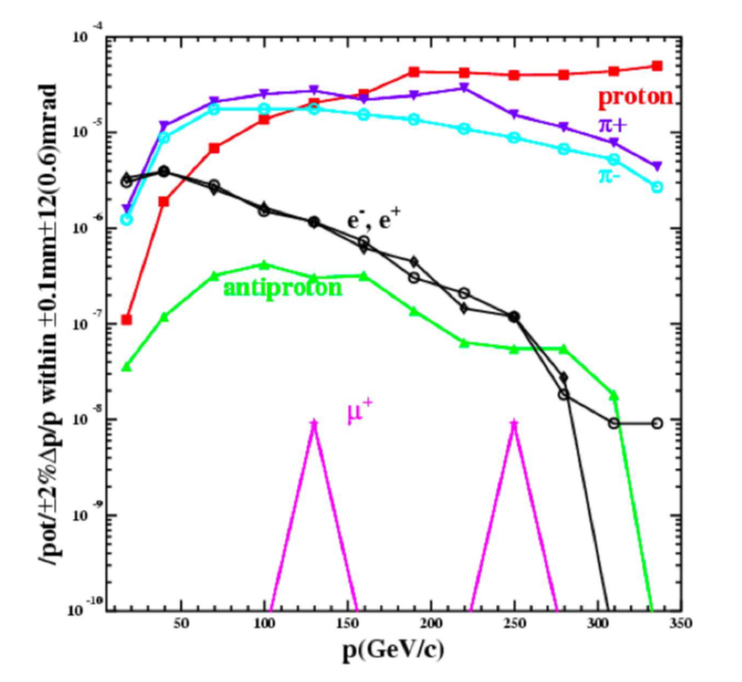
\includegraphics[width=0.5\textwidth]{productionrate.png}
	\hspace*{\fill}
	\caption{Beam intensity of H4 beam line from target T2 at SPS, CERN.}
	\label{fig:prodrate}
\end{figure}

One of the main background sources in the experiment is related to the possible presence of the low-energy tail in the
energy distribution of beam electrons. This tail was observed during irradiation of the setup by the \SI{100}{GeV}
electron beam without switching on the deflecting magnet. This tail is caused by the
electron interactions with a passive material, e.g. as entrance windows of the beam lines, residual gas, etc... Another
source of low energy electrons is due to the pion or muon decays in flight in the beam line. The uncertainties arising
from the lack of knowledge of the dead material composition in the beam line are potentially the largest source of
systematic uncertainty in accurate calculations of the fraction and energy distribution of these events. Hence, the
sensitivity of the experiment could be determined by the presence of such electrons in the beam, unless one takes
special measures to suppress this background. To reject these background sources at high energies by using standard
techniques,e.g. threshold Cerenkov counters, is practically impossible, see Section \ref{cerenkov}.\par

To improve the high energy electrons selections and suppress background from the possible admixture of low energy
electrons, we use a tagging system utilizing the synchrotron radiation (SR) from high energy electrons in a dipole
magnet, installed upstream of the detector. \par


\subsection{Physics Motivation}

\begin{equation}
{\cal L} = {\cal
L}_{SM}-\frac{1}{4}F'_{\mu\nu}F'^{\mu\nu}+\frac{\epsilon}{2}F'_{\mu\nu}F^{\mu\nu}+\frac{m^2_{A'}}{2}A_{\mu}'A'^{\mu}+i\bar{\chi}\gamma^{\mu}\partial_{\mu}\chi-m_{\chi}\bar{\chi}\chi-e_D\bar{\chi}\gamma^{\mu}A'_{\mu}\chi
\end{equation}
Standard Model.\\
$g_{\mu}-2$ muon anomaly\\
 


\subsection{Dark Photon signal}

U(1) broken symmetry $\longrightarrow$ massive dark photon\\
type of mixing
coupling constant and sub-GeV mass connect with g2 muon anomaly.
How to detect him?
\subsubsection{Visible decay}


\begin{figure}[ht]
	\hspace*{\fill}
	\centering
	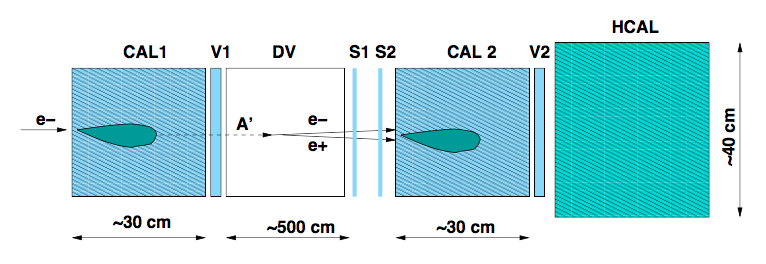
\includegraphics[width=0.5\textwidth]{schemevis.png}
	\hspace*{\fill}
	\caption{}
	\label{fig:schemevis}
\end{figure}

\begin{equation}
\mathrm{S_{A'} = CAL1 \cdot \overline{V1}\cdot S1\cdot S2\cdot CAL2\cdot \overline{V2}\cdot\overline{HCAL}}
\end{equation}

\begin{figure}[ht]
	\hspace*{\fill}
	\centering
	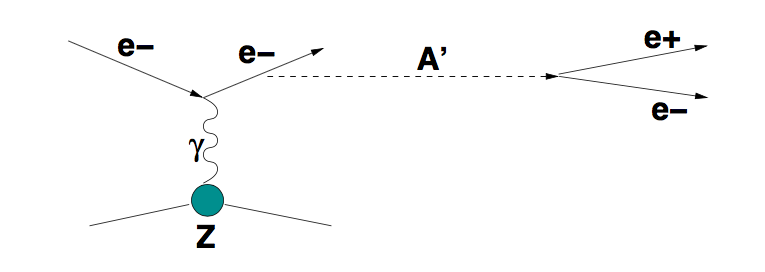
\includegraphics[width=0.5\textwidth]{visible.png}
	\hspace*{\fill}
	\captionsetup{margin=1cm}
	\caption{Diagram illustrating the massive $A'$ production in the reaction $e^-Z\rightarrow e^-ZA'$ of electrons
	scattering off a nuclei ($A$, $Z$) with the subsequent $A'$ into an $e^+e^-$ pair.}\label{fig:vis}
\end{figure}


\subsubsection{Invisible decay}
\begin{figure}[ht]
	\hspace*{\fill}
	\centering
	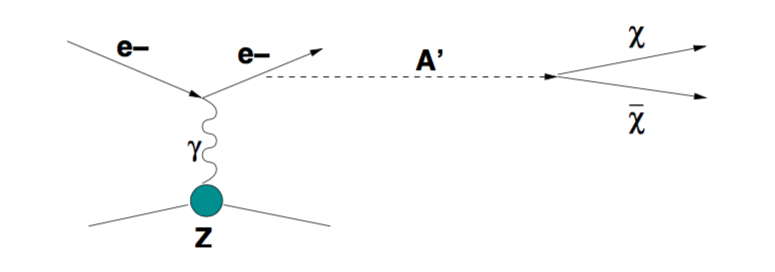
\includegraphics[width=0.5\textwidth]{invisible.png}
	\hspace*{\fill}
	\caption{Production rate at H4 beam line}\label{fig:inv}
\end{figure}

\begin{figure}[ht]
	\hspace*{\fill}
	\centering
	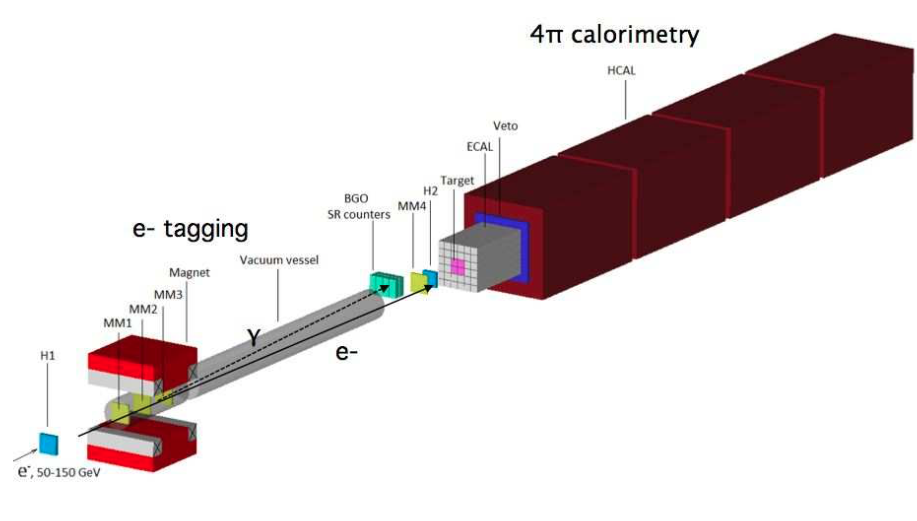
\includegraphics[width=0.8\textwidth]{schemeinv2.png}
	\hspace*{\fill}
	\caption{Illustration of detector configuration for Invisible decays of Dark photon.}\label{fig:schemeinv}
\end{figure}

The method of the search is the following. The incident electron energy absorption in the ECAL is accompanied by the
emission of bremsstrahlung $A'$s in the reaction $eZ\rightarrow eZA'$ of electrons scattering on nuclei, due to the
$\gamma - A'$ mixing. The diagram for the $A'$ production in the reaction is shown in Figure \ref{fig:inv}.\par

The reaction typically occurs in the first few radiation length ($X_0$) of the calorimeter (ECAL0). The part of the primary beam
energy is deposited in the ECAL, while the remaining fraction of the total energy is transmitted by light dark matter
decay particles $\chi$ through the rest of the detector. The $\chi$ penetrates the ECAL, veto V and the HCAL without
interactions resulting in the missing-energy signature in the detector.\par

The occurrence of $A'\rightarrow invisible$ decays produced in $e^-Z$ interactions would appear as an excess of events
with a single electromagnetic shower in the ECAL1,Fig. \ref{fig:schemeinv}, and zero energy deposition in the rest of
the detector (V and HCAL), above those expected from the background sources. The signal candidate events have the
signature:\par



\begin{equation}
\mathrm{ S_{A'} = H1 \cdot H2\cdot ECAL (E_{ECAL}<E_0)\cdot \overline{V\cdot HCAL}}
\end{equation}

and should satisfy the following selection criteria:

\begin{itemize}
\item The momentum of the incoming particle track should correspond to the beam momentum.
\item The starting point of (e-m) showers in the ECAL should be localized within a few first $X_0$s.
\item The lateral and longitudinal shapes of the shower in the ECAL are consistent with an electromagnetic one. The
fraction of the total energy deposition in the ECAL is $f<0.5$.
\item No energy deposition in the V and HCAL.
\end{itemize}

To improve the primary high energy electrons selection and additionally suppress background from the possible presence
of low energy electrons in the beam typically with energy $E_e <0.5 E_0$ (see below), one use a high energy $e^-$ tagging
system utilizing the synchrotron radiation (SR) from high energy electrons in a dipole magnet, as schematically shown in
Fig. \ref{fig:schemeinv}. 




\subsection{Detector}

The $A'$ production is a rare event. For the interesting parameter range it is expected to occur with a rate $10^{-9}$
with respect to the ordinary photon production rate. Hence, its observation represents a challenge for the detector
design and performance.\par

The experimental setup specifically designed to search for the $A'$ production in the reaction (4) of high-energy
electron scattering off nuclei in a high density target T is schematically shown in Fig. 3. The experiment employs the
upgraded H4 electron beam line at the CERN SPS described in details in Ref.\cite{sps}. The beam is designed
to transport the electrons with the maximal intensity $\simeq (3-4) \cdot 10^6$ per SPS spill in the momentum range
between \SIrange{50}{150}{GeV/c} that could be produced by the primary proton beam of \SI{450}{GeV/c} with the intensity
up to a few $10^{12}$ protons on target. The electrons are produced by protons impinging on a primary beryllium target and
transported to the detector inside the evacuated beam-line tuned to an adjustable beam momentum. \par

The hadron contamination in the electron beam is $\pi/e < 10^{-1}-10^{-2}$ and the size of the beam at the detector position is
of the order of a few \si{\square\centi\metre}.

The detector shown in Figure \ref{fig:na64detector} utilizes upstream magnetic spectrometers (MS) consisting of dipole
magnets and a low-material-budget tracker, which is a set of Micromegas chambers , MM1-MM4 (T1-T4 in the figure),
allowing the reconstruction and momentum resolution at 100 GeV $\Delta P/P\sim 2\%$ for incident electrons \cite{mm}. It
also uses the scintillating counters S0, S1 and hodoscopes H1 and H2 to define the primary beam, and the active target
T, which is the central part of the high-efficiency hodoscopic electromagnetic calorimeter (ECAL) used for the accurate
measurement of the recoil electron energy from the reaction (4). Downstream the target the detector is equipped with
high-efficiency forward veto counter V, and a massive, completely hermetic hadronic calorimeter (HCAL). Three
straw-tubes chambers, MUON1-MUON3, located between the HCAL modules are used for the final-state muon(s) identification.
The modules serve as a dump to completely absorb and detect the energy of hadronic secondaries produced in the electron
interactions $e^-A\rightarrow anything$ in the target. In order to suppress backgrounds caused by the detection
inefficiency the HCAL must be longitudinally completely hermetic [18, 19]. To enhance its hermeticity, the HCAL
thickness is chosen to be $\simeq  30 \lambda_{\mathrm{int}}$ (nuclear interaction lengths). The 15 m long vacuum vessel
between the magnet and the ECAL is installed to avoid absorption of the synchrotron radiation photons detected at the
downstream end of the vessel by the array of BGO crystals for the effective tagging of the incoming beam electron.



\begin{figure}[ht]
		\hspace*{\fill}
		\centering
		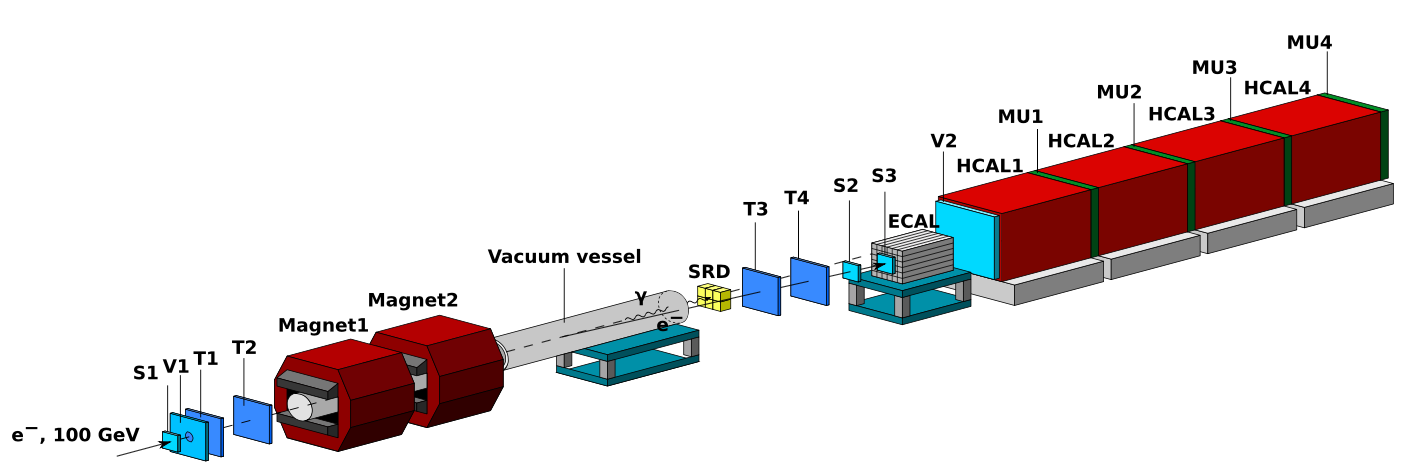
\includegraphics[width=\textwidth]{na64detector.png}
		\captionsetup{margin=1cm}
		\caption{Schematic illustration of the setup to search for $A'\rightarrow${\it invisible} decays with 100GeV e$^-$
		at H4 beam line. the incident electron energy absorption in the ECAL is accompanied by the emission of
		{\it bremsstrahlung} $A'$s in the reaction $eZ\rightarrow eZA'$ of electron scattering on nuclei, see Diagram
		interaction. The part of the primary beam energy is deposited in the ECAL, while the remaining fraction of the total
		energy is transmitted by the decay dark matter particles through the rest of the detector resulting in the missing
		energy signature in the detector.}\label{fig:na64detector}
\end{figure}



%------------------- SYNCHROTRON RADIATION  SYSTEM ------------------


\section{The synchrotron radiation tagging system}
\textcolor{red}{The basic idea is that, since the critical SR photon energy is $(\hbar
\omega)_{\gamma}^c \propto E_0^3$, the low energy electrons in the beam could be rejected by using the cut, e.g.
$E_{\gamma}>0.3(\hbar\omega)_{\gamma}^c$, on the energy deposited in the SR detector. }

One of the main background sources in the experiment is related to the possible presence of the low-energy tail in the
energy distribution of beam electrons. Indeed, this tail was immediately observed during irradiation of the setup by the
100GeV electron beam without switching on the deflecting magnet (see Figure \ref{fig:electrontail}). This tail is caused
by the electron interactions with a passive material, such e.g. as entrance windows of the beam lines, residual gas,
etc... Another source of low energy electrons is due to the pion or muon decays in flight in the beam line.\par

The uncertainties arising form the lack of knowledge of the dead material composition in the beam line are potentially
the largest source of systematic uncertainty in accurate calculations of the fraction and energy distribution of these
events.\par

An estimation shows that the fraction of events with energy below $\lesssim 10$GeV in the electron beam tuned to 100GeV
could be as large as $10^{-8}$. Hence, the sensitivity of the experiment could be determined by the presence of such
electrons in the beam, unless on takes special measures to suppress this background. \par


\begin{figure}[ht]
	\hspace*{\fill}
	\centering
	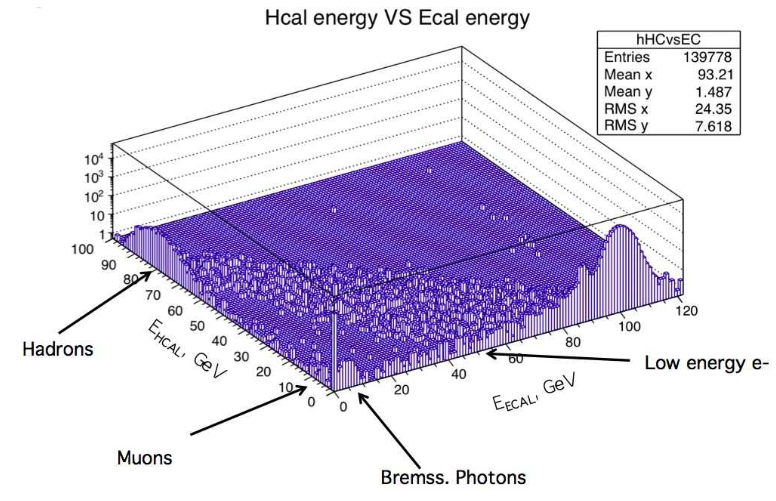
\includegraphics[width=0.8\textwidth]{electrontail.png}
	\hspace*{\fill}
	\caption{Distribution of 100GeV $e^-$ events in the ($\mathrm{E_{HCAL};E_{ECAL}}$) plane. }
	\label{fig:electrontail}
\end{figure}


%------------------- CHERENKOV RADIATION ------------------

\subsection{Cherenkov Radiation}\label{cerenkov}

To reject these background sources at high energies by using standard techniques, such as threshold Cherenkov counters,
is practically impossible. The use of Cherenkov radiation allows to identify the particles by their mass. This type of
electromagnetic radiation is emitted when a charged particle passes through a dielectric medium at speed $v$ greater
than the phase velocity of light $c/n$, where $n$ is the refraction index of the medium. Hence, the condition to emit
Cherenkov radiation is when:

\begin{equation}\label{condCR}
\frac{v}{c} = \beta > \frac{1}{n} 
\end{equation}

In a beam line, the particles are selected by their momentum $P$, therefore particles with different mass would have the
same momentum. For a relativistic particle the velocity $\beta$ can be written in terms of its momentum and total energy
$E$:
\begin{equation}
\beta=1/\sqrt{1+\left(m/P\right)^2}
\end{equation}

where $m$ is the mass of the particle. Therefore, the selection of the particles (with different mass) can be done
changing the threshold of Cherenkov radiation using a proper medium with a refraction index $n$ which allows the
selection from $\beta_1$ and $\beta_2$. The medium selected must have a refraction index $n$ such as $\beta_1(m_1)>1/n$ and
$\beta_2(m_2)<1/n$, where $m_1>m_2$. But for a 100GeV momentum $\beta_{\pi}\simeq\beta_{e}$ and an index refraction
which satisfy the condition $\beta_1>1/n_{max}$ where $n_{max}\simeq 1.000000979$ and should be higher than $n_{min}\simeq
1.00000000001$  thus the method is inefficient for this range of energy.\par


%------------------- SYNCHROTRON  RADIATION ------------------

\subsection{Synchrotron Radiation}

Another technique to reject heavy charged particles is the use of synchrotron radiation which exploit the high
suppression of the radiated power emitted by particles heavier than electrons passing through a magnetic field in order
to discriminate them.  The use of this technique is not new and detection of electrons or positrons in electrons beams
with momenta ranging from 30 to 50 GeV was reported earlier by \cite{srd1,srd2,srd3}.\par

For synchrotron radiation we understood when a charged particle in a magnetic field moves in a circular motion emitting
photons along its trajectory due to the basic principles of electrodynamics. Both quantum and classical theory of
synchrotron radiation (SR) are well understood \cite{synchrotron}. In the range of interest for our experiment both
treatments are equivalent and we can therefore use the classical approximation for our calculations. The total power $P$
emitted per unit length by a relativistic charged particle of energy $E$ with mass $m$ and with bending radius $R$ in a
magnetic field $B$ perpendicular to its velocity is given by:


\begin{equation}
P = \frac{q^2c}{6\pi}\frac{1}{(mc^2)^4}\frac{E^4}{R^2}
\end{equation}

where $q$ is the charge of the particle and $c$ the speed of light. Since the emission angle of the synchrotron is
proportional to the inverse of the Lorentz factor $\gamma$, the photons are emitted tangentially to the particle
trajectory.\par

Hence under a circular acceleration, an charged particle, e.g. an electron, emits synchrotron radiation and the energy
radiated per particle per turn being

\begin{equation}
\Delta E = \frac{e^2\beta^3}{3\varepsilon_0 R}\left (\frac{E}{mc^2}\right )^4
\end{equation}
Putting the numerical values for $\varepsilon_0$ and $e$, and setting $\beta=1$

\begin{equation}
\Delta E = 0.08856\frac{E^4}{R}
\end{equation}

\begin{figure}[htbp]
\begin{center}
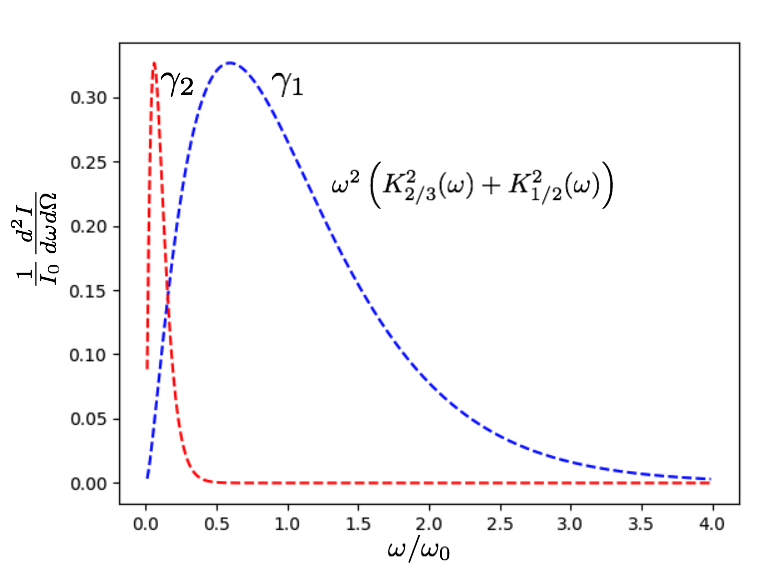
\includegraphics[width=0.6\textwidth]{spectrumSR.png}
\caption{Spectrum synchrotron radiation from two different particles, where $\gamma_{1}=10\gamma_{2}$}
\label{default}
\end{center}
\end{figure}

where $\Delta E$ is in \unit{MeV}, $E$ is in \unit{GeV} and $R$ is in meters. Thus for relativistic $\pi^-$'s and
$e^-$'s of the same energy, the energy loss is $(m_e/m_{\pi^{\pm}})^4\sim 10^{-10}$ times less for a $\pi^{\pm}$. This
would be the case if the particles propagate in an ideal vacuum. However, in a real experimental setup, vacuum windows,
residual gas, beam counters such as scintillators and trackers result in interactions of the incoming particles with
material. Therefore, the suppression factor when crossing materials is limited by the emission of secondary electrons
with enough kinetic energy (several MeV) to leave a synchrotron-like signal in the detector. Although most of the energy
transfer due to ionization for heavy charged particles is only a few keV, rare high energy transfer is possible. The
distribution of such secondary electrons with kinetic energy $T>>I$, where $I$ is the mean excitation energy of the
atom/molecule, for a particle with velocity $\beta$ and charge $z$ passing through a material with atomic number $Z$,
mass number $A$ and thickness $dx$ is described by PDG.

\begin{equation}
\frac{d^2N}{dTdx}=\frac{1}{2}Kz^2\frac{Z}{A}\frac{1}{\beta^2}\frac{F(T)}{T^2}
\end{equation}

The constant $K$ is defined as $K=4\pi N_A r^2_em_ec^2$ where $N_A$ is the Avogadro's number, $r_e$ is the classical
electron radius and $m_e$ the electron mass. $F(T)$ is a spin-dependent factor, which in our case for $T<<W_{max}$ is
very close to unity. $W_{max}$ is the maximal energy transfer in a single collision to the electron:

For a $\pi^-$ at \si{\giga\electronvolt}, $W_{max}$ is roughly 1\si{\giga\electronvolt} which covers completely the
energy range where synchrotron radiation is emitted. 


\begin{figure}[ht]
	\hspace*{\fill}
	\centering
	\includegraphics[width=0.5\textwidth]{schemeSRD.pdf}
	\hspace*{\fill}
	\captionsetup{margin=1cm}
	\caption{The scheme of the additional tagging of high energy electrons in the beam by using the electron synchrotron
	radiation in the bending magnetic dipole. The synchrotron radiation photons are detected by a $\gamma$-detector by
	using scintillator as BGO crystals, LYSO crystals or a different configuration with Pb+Sc. All theses options are viewed
	by a high quantum efficiency PMT or SiPM. The beam defining counters are also shown.}
	\label{}
\end{figure}


For 100GeV electrons in the $B=1.7$T bending field this corresponds to $E_c \sim 11.35$MeV. The expected mean energy of
a synchrotron photon $E_m=E_c/\pi \simeq 3.6$MeV is in very good agreement with simulation. The number of photons
emitted per revolution in this energy range in the field of 7T$\cdot$m is defined as:

\begin{equation}
N_{\gamma's} = \frac{5\pi\alpha}{\sqrt{3}}\gamma
\end{equation}

where $\alpha$ is the fine structure. By scaling this equation for the fraction of the circle where the particles are
inside the magnetic field, one obtains a mean number of emitted photon of about 24. Afterwards we should consider the
geometrical acceptance of the SRD to estimate the total energy deposited in the detector.\par

To detect this SR, the experiment has been working to find the best suitable detector. For this task three options has
been tested, three type of scintillator material; BGO, LYSO and Pb+Sc. Each of one with different geometry and
crystal's configuration. On this thesis we focus only on two out of the three options, BGO and LYSO due to its
similarities and good perfomance. A description of
these detector can be found on the next sections and a comparison of how can be used to suppress the hadron contamination on the beam
line.\par

%----------------------------- BGO ----------------------------- 

\subsection{BGO}\label{bgoanal}

The NA64 experiment, use as a first option of SRD an array of $\mathrm{Bi_4Ge_3O_{12}}$ (BGO) crystals because of its
high photoelectric gamma rays absorption and a configuration that can the detect the incoming SR and reject the back
scattering event coming from the ECAL.\par

\begin{figure}[ht]
	\centering
	\hspace*{\fill}
	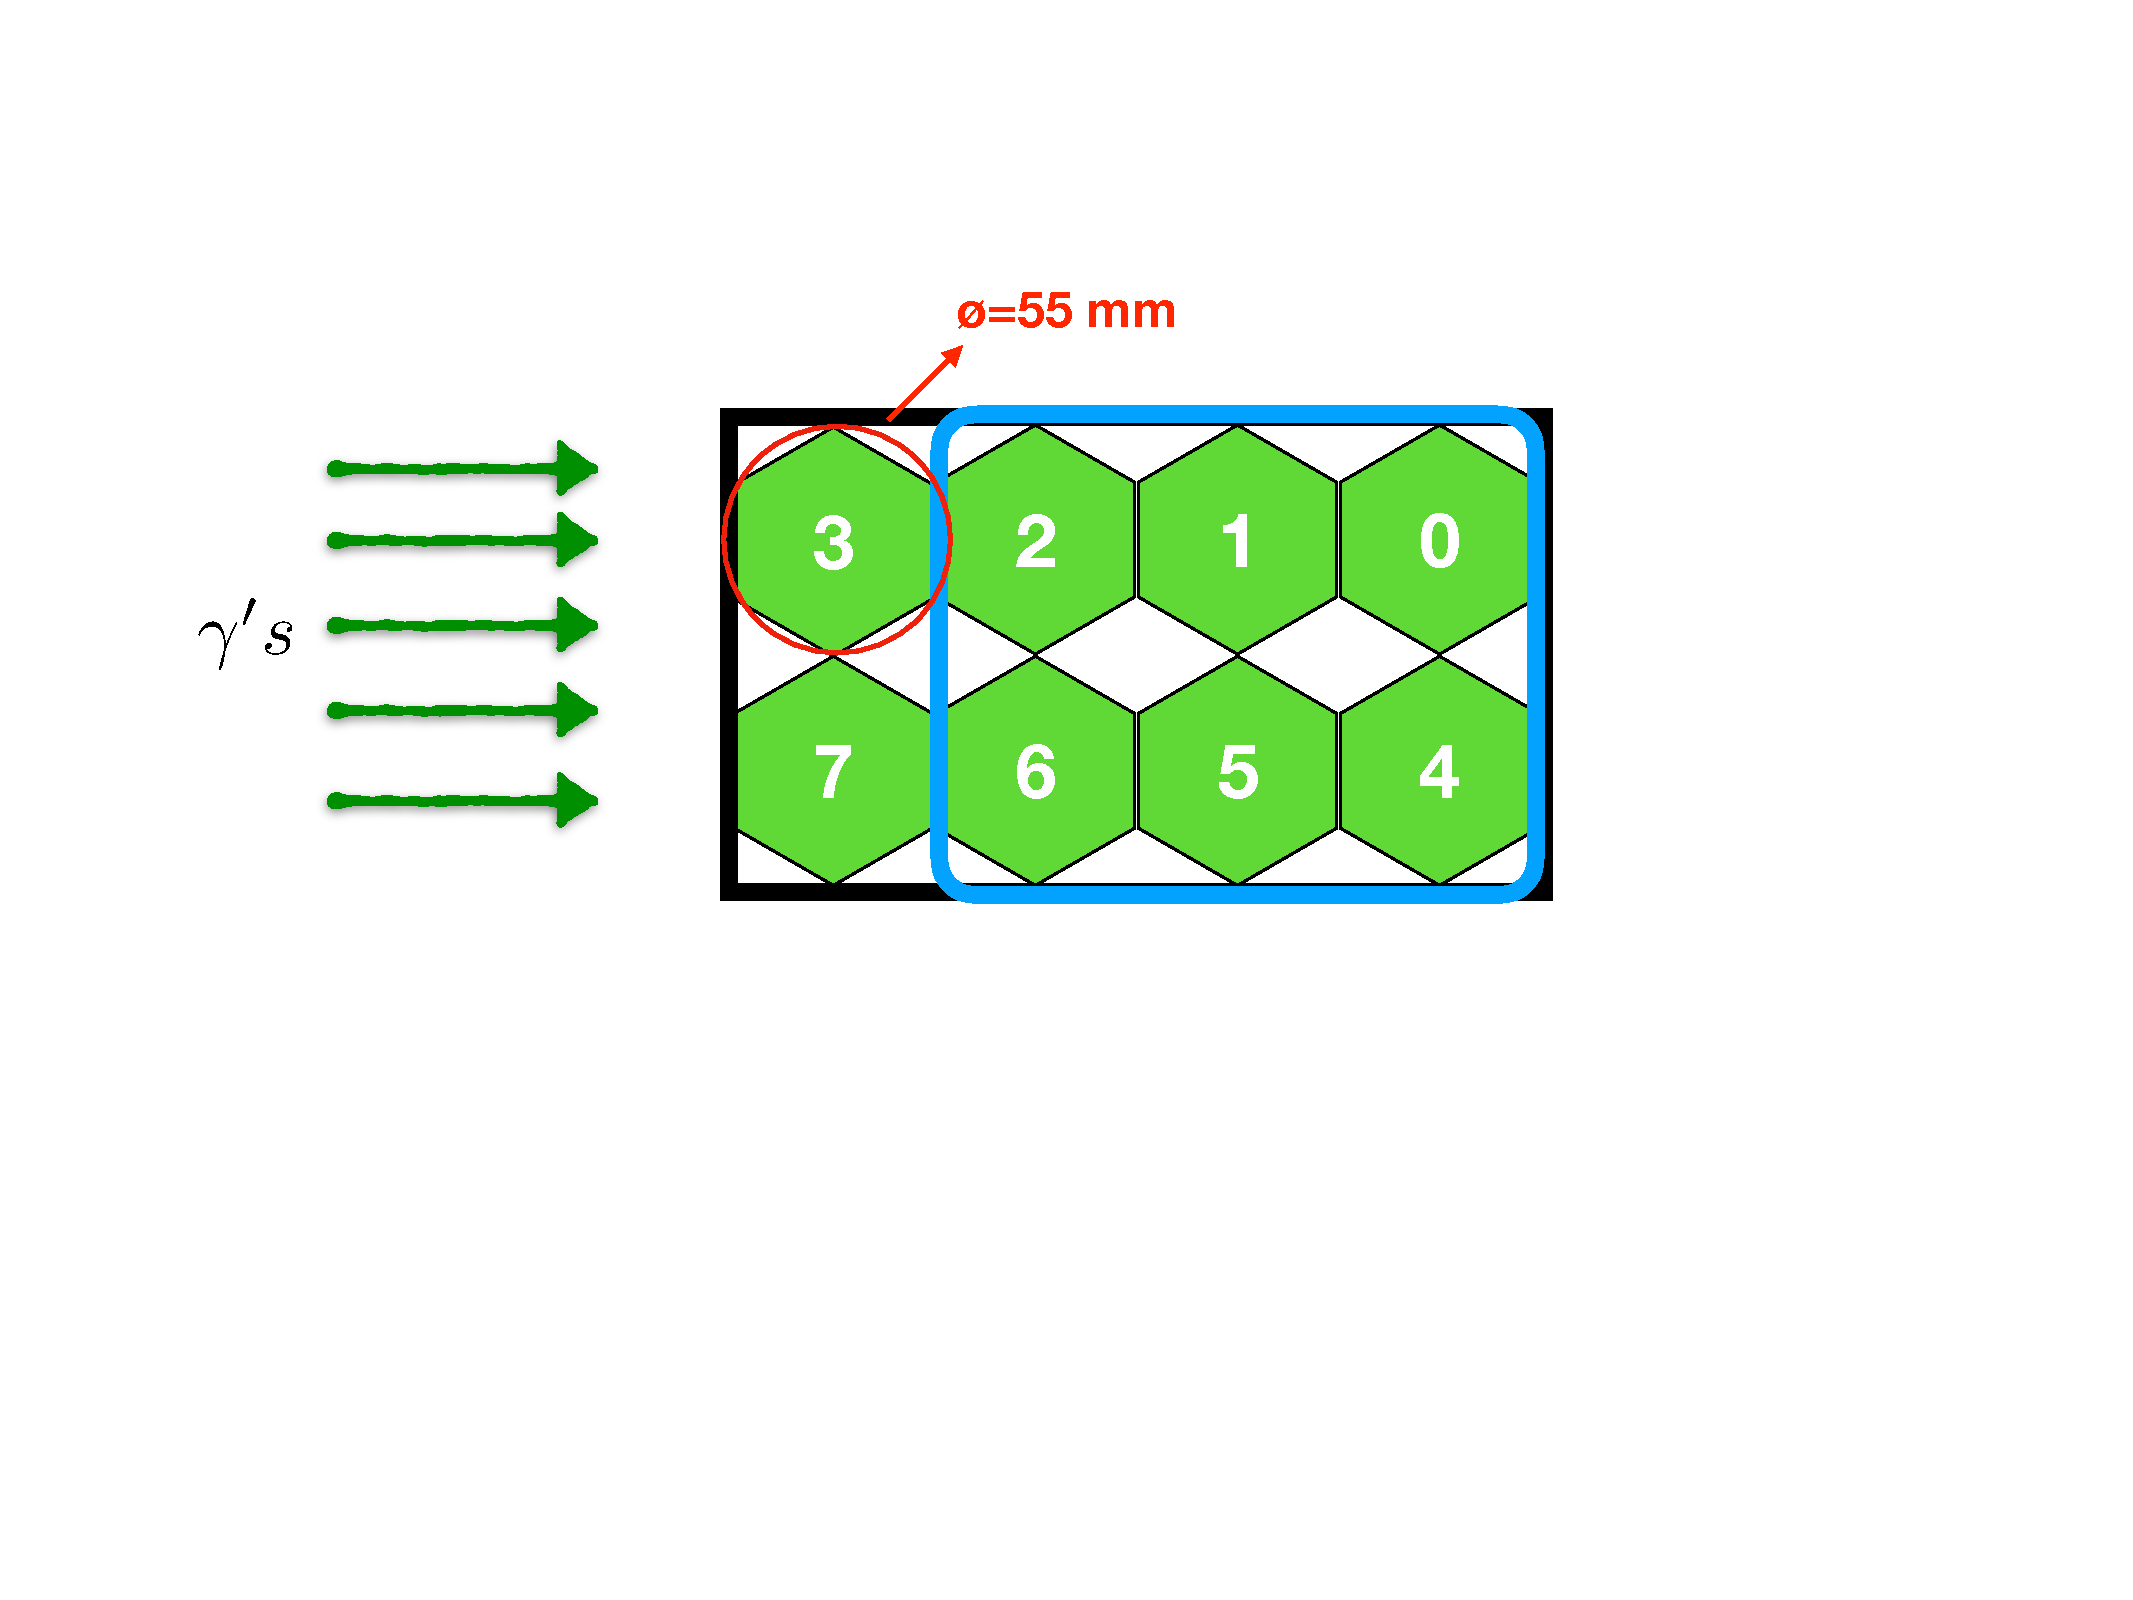
\includegraphics[width=0.5\textwidth]{bgoscheme.pdf}
	\hspace*{\fill}
	\captionsetup{margin=1cm}
	\caption{Detector BGO, array of 8 hexagonal crystals with 55mm external diameter and 200mm length. .}\label{bgoscheme}
\end{figure}

The detector consists of 8 hexagonal crystals with an external diameter of \SI{55}{mm} and a length of \SI{200}{mm} (see
Figure \ref{bgoscheme}). The first two crystals collect most of the synchrotron radiation spectrum. The las two crystals
are affected only in case of a high energy event and rare thus uses as a veto. The remaining crystals (square light
blue) serve as a shield for the SRD from backscattering particles coming from the ECAL. The crystals are grouped into
two modules. Each crystal is wrapped in Teflon tape for efficient light collection and it is glued to an ETL 9954
photomultiplier(PMT).\par


The BGO crystal has a density of 7.13 \si{\gram/\centi\cubic\metre} and because of the high atomic number of the bismuth
component ($Z=83$) it has one of the larges probability per unit volume for photoelectric absorption of gamma rays.
\cite{bgodatashet}. The light yield of about 8500 $\gamma$s/MeV coupled to the transportation losses and
quantum efficiency of the PMT gives an energy resolution of about 17\% (FWHM) at \SI{1.27}{MeV} (measured with a
$\mathrm{^{22}Na}$ radioactive source).\par


%----------------------------- LYSO  ----------------------------- 
\subsection{LYSO}

The setup for invisible decays has differents scintillating material to detect synchrotron radiation. An array of
LYSO\cite{lysogobain} crystals.  This array consists of 25x25 crystals of 4x4x45 \si{\cubic\milli\metre} each crystal is
a Cerium doped lutetium ($\mathrm{Lu_{1.8}Y_{0.2}SiO_5:Ce}$), with a light output of 35.000 [photons/MeV].  This type of
crystals has a short time decay (see Table \ref{property}) compared to BGO crystals.  Therefore, it is a more suitable
candidate for a SR detection at high rates. With a decay time of $\tau=40$ns, allows to a maximal electron counting rate
of $\lesssim 1/\tau \sim 10^7 e^-/s$.\par

\begin{figure}[hb]
	\hspace*{\fill}
	\centering
		\begin{subfigure}[b]{0.45\textwidth}
			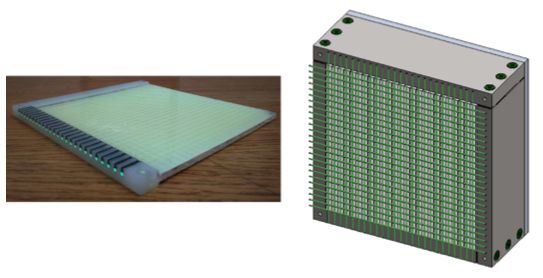
\includegraphics[width=\textwidth]{preshower.png}
			\caption{}\label{uvtnet}
		\end{subfigure}
		\hfill
		\begin{subfigure}[b]{0.45\textwidth}
			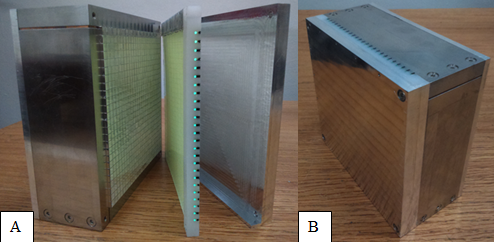
\includegraphics[width=\textwidth]{ps_closing.png}
			\caption{}\label{housing}
		\end{subfigure}
\hspace*{\fill}
	\caption{LYSO detector}\label{preshower}
\end{figure}

\begin{table}[ht]\footnotesize
\centering
\begin{tabular*}{0.6\textwidth}{lcc}
Property & LYSO & BGO\\
\hline Density [\SI{}{g/m^3}]				& 7.1 	& 7.1 \\
Attenuation length for 511 keV [cm] & 1.2 	& 1.0\\
Decay time [ns]	 										& 41 		& 300\\
Energy Resolution \% 								& 8.0 	& 12.0\\
Light output, photons per keV 			& 32 		&	9 \\
Radiation Length										& 1.16 	& 0.96\\
\end{tabular*}
\caption{Property comparison LYSO and BGO crystals}\label{property}
\end{table}

The light spectrum emission from LYSO crystals hast its peak at \SI{420}{nm}, this light is collected from a net of
KURARAY Y-7  wave length shifter (WLS) fibers. This WLS has its maximum of light absortion at 439nm and 490nm of its
peak emission. The net of fibers are mounted in a UVT acrylic (see Figure \ref{uvtnet}) and at the end of each WLS there
is a small light guide connected to a Multi-pixel photon counter (Hamamatsu S10931-025P) to measure the photons
collected. This type of Avalanche photo diode it suit perfect for the emission of the WLS due to its photon detection
efficiency (PDE) maximum (50\%) is close to 490nm.\par 

Each crystal is wrapped in a ultra high reflective film Vikuiti and assambled in an aluminum housing as shows the Figure
\ref{housing}. The light collection is taking only from one side from this array. On Figure \ref{housing} is possible to
observe the end of each 25 fibers from one side. Once the housing is closed the electron readout are mounted on top and
on one side of this box shape. This design of about 4$X_0$ can be used as a preshower detector with a compact volume and
high dense transversal segmentation.  \par

\subsubsection{Readout}

\begin{figure}[t]
	\hspace*{\fill}
	\centering
	\begin{subfigure}[b]{0.45\textwidth}
	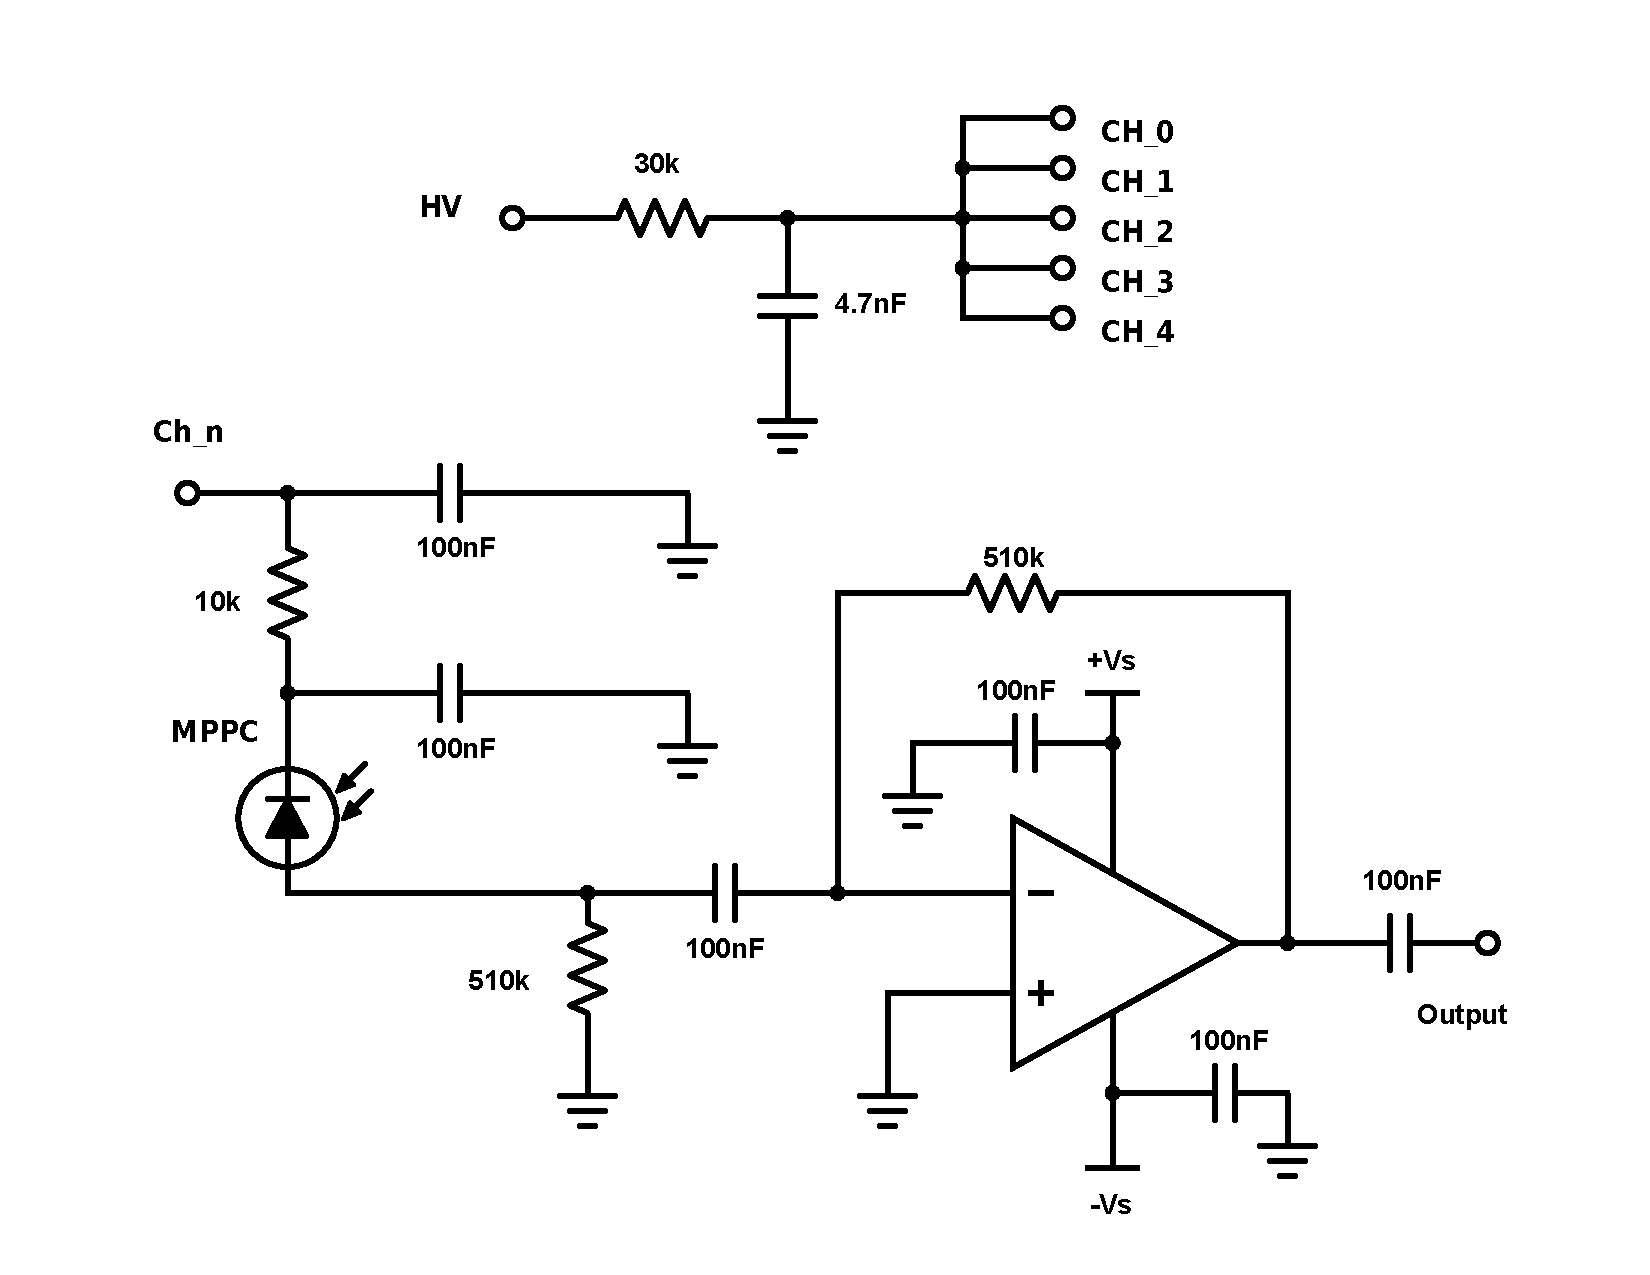
\includegraphics[width=\textwidth]{circuit.pdf}
	\caption{Amplifier and bias voltage circuit for MPPC}\label{scheme}
	\end{subfigure}
	\begin{subfigure}[b]{0.45\textwidth}
	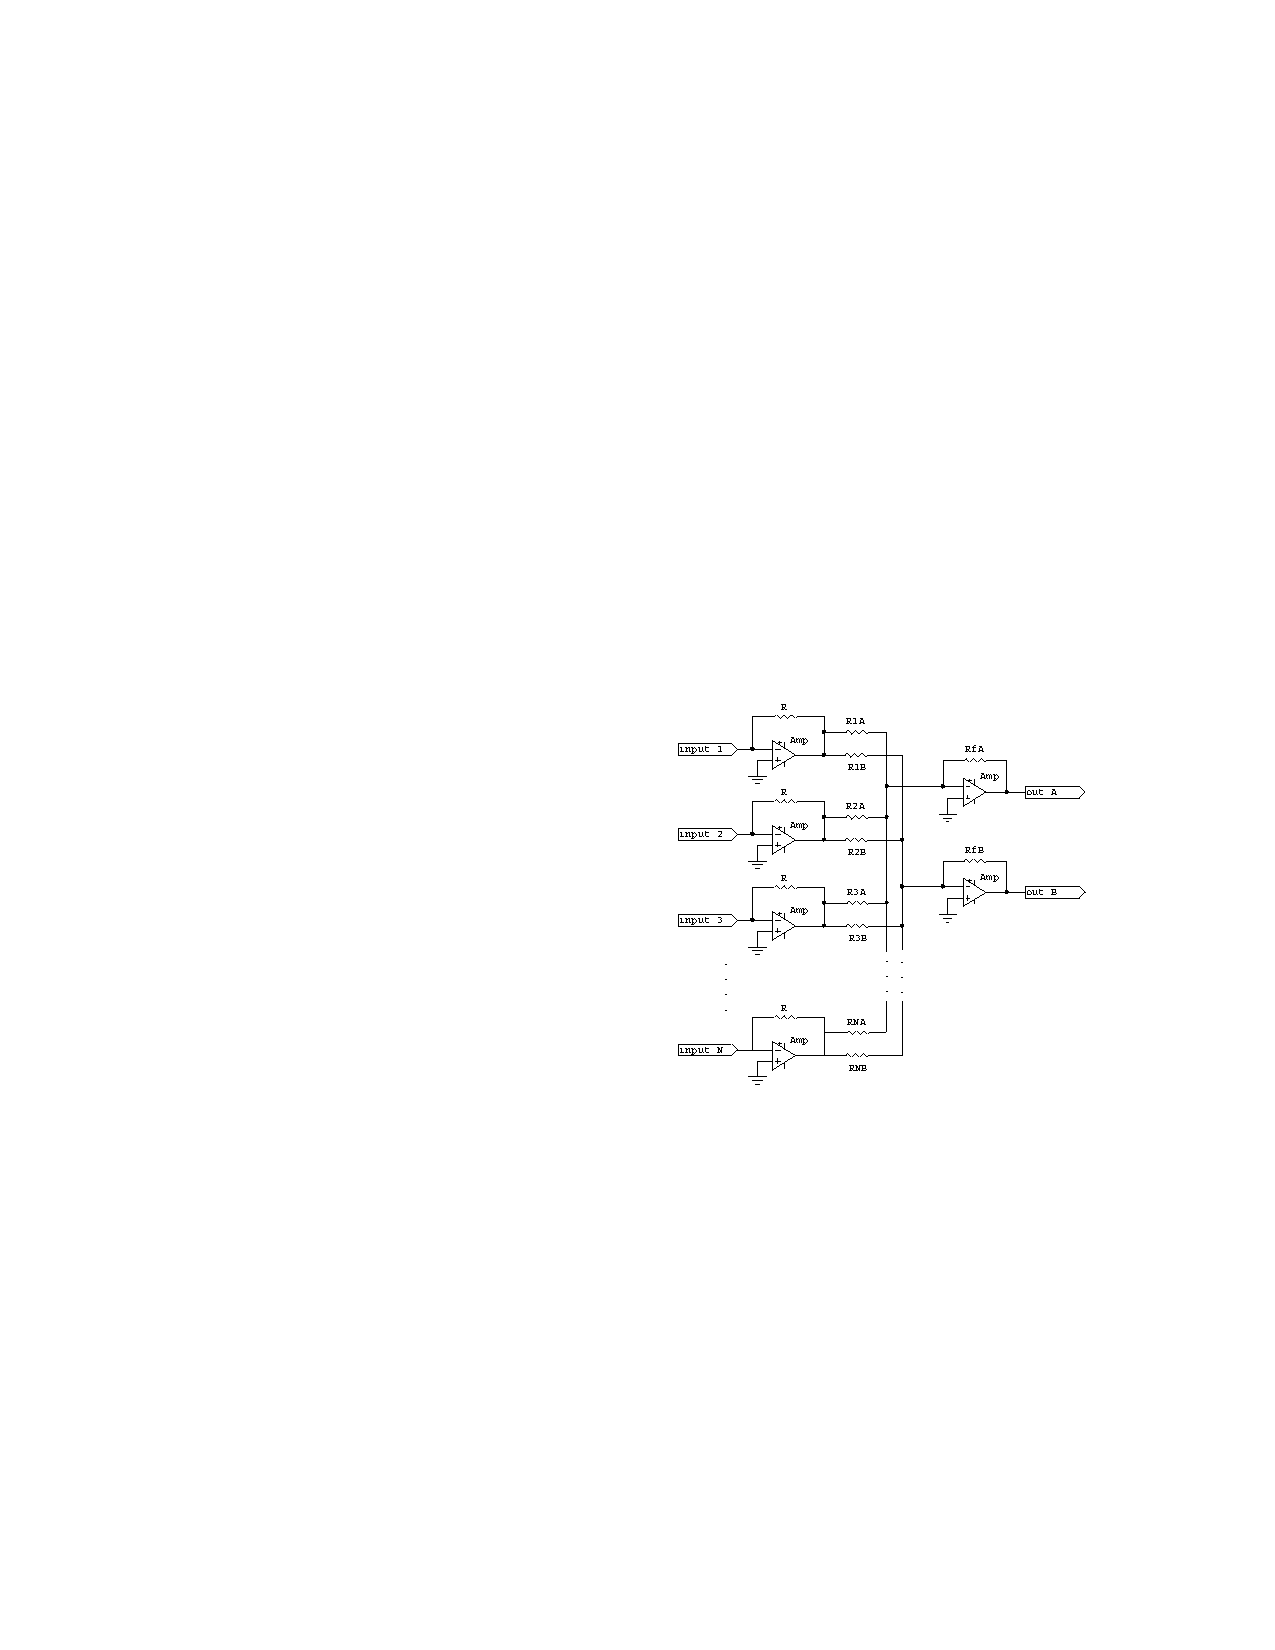
\includegraphics[width=\textwidth]{sumab.pdf}
	\captionsetup{margin=1cm}
	\caption{Weighted signal circuit}\label{sumab} 
	\end{subfigure}
	\hspace*{\fill}
	\caption{The figure {\bf(a)} shows two circtuis, one the amplifier circuit (bottom) fro each Multi-Pixel Photon Counter. On
	top is the common bias voltage for 5 channels. The circuit on {\bf(b)} provides the two weighted signal from $N$ channels which is
	implemented on one side of this detector to reduce the amount of channels.}\label{circuits}
\end{figure}

The readout consists of 50 Multi-pixel Photon Counter (MPPC) \cite{mppc}, distributed into 25 per axis (X and Y). The 25
MPPC from each axis were selected to share the same bias voltages in group of 5 with similar gain. However the signal
output comes from the 25 photon counters. The Figure \ref{scheme} shows the amplification circuit for each MPPC and the
circuit which connect the 5 neighbor MPPC to the same bias voltage.\par

The high transversal segmentation (4mmx4mm) from this device can help to identify the particle position and its energy
very accurate. However, its disadvantage is the amount of channels need it for this purpose.\par

The lack of free ADC channels in the NA64's DAQ system lead us to reduce the channel numbers. Since the electron beam will
be deviated only horizontally, the SR accros should be homogenosly distributed across the x-axis. Therefore, to identify
other events, with low SR emission like pions or delta electrons it is much better to keep the advantage of the 25
channels. On the other hand, the use of a charge division readout sytem on the y-side can help to reduce from 25 to two
analog output signals. \par

This readout system operates as a multi-channel analog signal converter which converts signals from
multi-channel output position sensitive devices to two per coordinate analog outputs with same amplitude correlation as
common charge division position readout.\par

For the experiment NA64, the readout was downgrade from 50 to 27 channels.  25 from the X axis were
kept and 2 weighted signals are obtained from 25 channels from Y axis. Two main reasons lead us to the this downgrade,
the first one is due to the limited number of channels of the DAQ system, and the second one is there is no need for
such high position resolution for the synchroton photons or low energy electrons, since the angle aperture from SR is
$\Delta \phi_{SR}\sim 1/\gamma$ and homogenous.\par

\begin{equation}\label{rarb}
R_n A = \frac{ R_f A}{ (n-1)\frac{G-1}{N-1}+1} \qquad R_n B = \frac{ R_f B}{ (N-n)\frac{G-1}{N-1}+1}
\end{equation}

To provide two weighted signals, an extra circuit is added with a charge division style (See Figure \ref{sumab}). This
circuit take the 25 signal output from each MPPC and provide two signals $A$ and $B$, each one depending on the Gain $G$
and the resistance $R_n$ where $n$ is the n-th channel. The equation for proper resistance for $N$ channels are provided
in equation \ref{rarb}.\par

The average of $A$ and $B$ provide the total amplitud recorded on the 25 channels while equation \ref{AplusB} shows the
position of the event ranged from 0 until $N$.

\begin{equation}\label{AplusB}
X = \frac{A-B}{A+B}
\end{equation}


\section{Calibration}

For the calibration the LYSO detector was installed on the NA64 detector on RUN I (July 2016). The detector is placed
right in front of the ECAL to profit from the trigger and the beam setup. Since it is the first time the detector is
connected to the DAQ\cite{compass}, a proper gain equalization must be performed. For this purpose, the detector was
placed in three different positions refer to the beam as it shows the Figure \ref{mip}. The first configuration (a),
allows us to equalized the 25 channels on the X-axis. A beam with pions will hit one crystal lossing its energy by
ionisation, wichi for high particles the minimom ionization is roughly \SI{2}{MeV/gcm^2}. Hence the total energy
deposition per channels is the width of each crystal (\SI{0.4}{cm}) times the LYSO density (\SI{7.1}{g/cm^3}) and the
loss energy per density (\SI{2}{MeV/gcm^2}) resulting in a \SI{5.68}{MeV}.

\begin{figure}[ht]
	\hspace*{\fill}
	\begin{subfigure}[b]{0.45\textwidth}
	\centering
	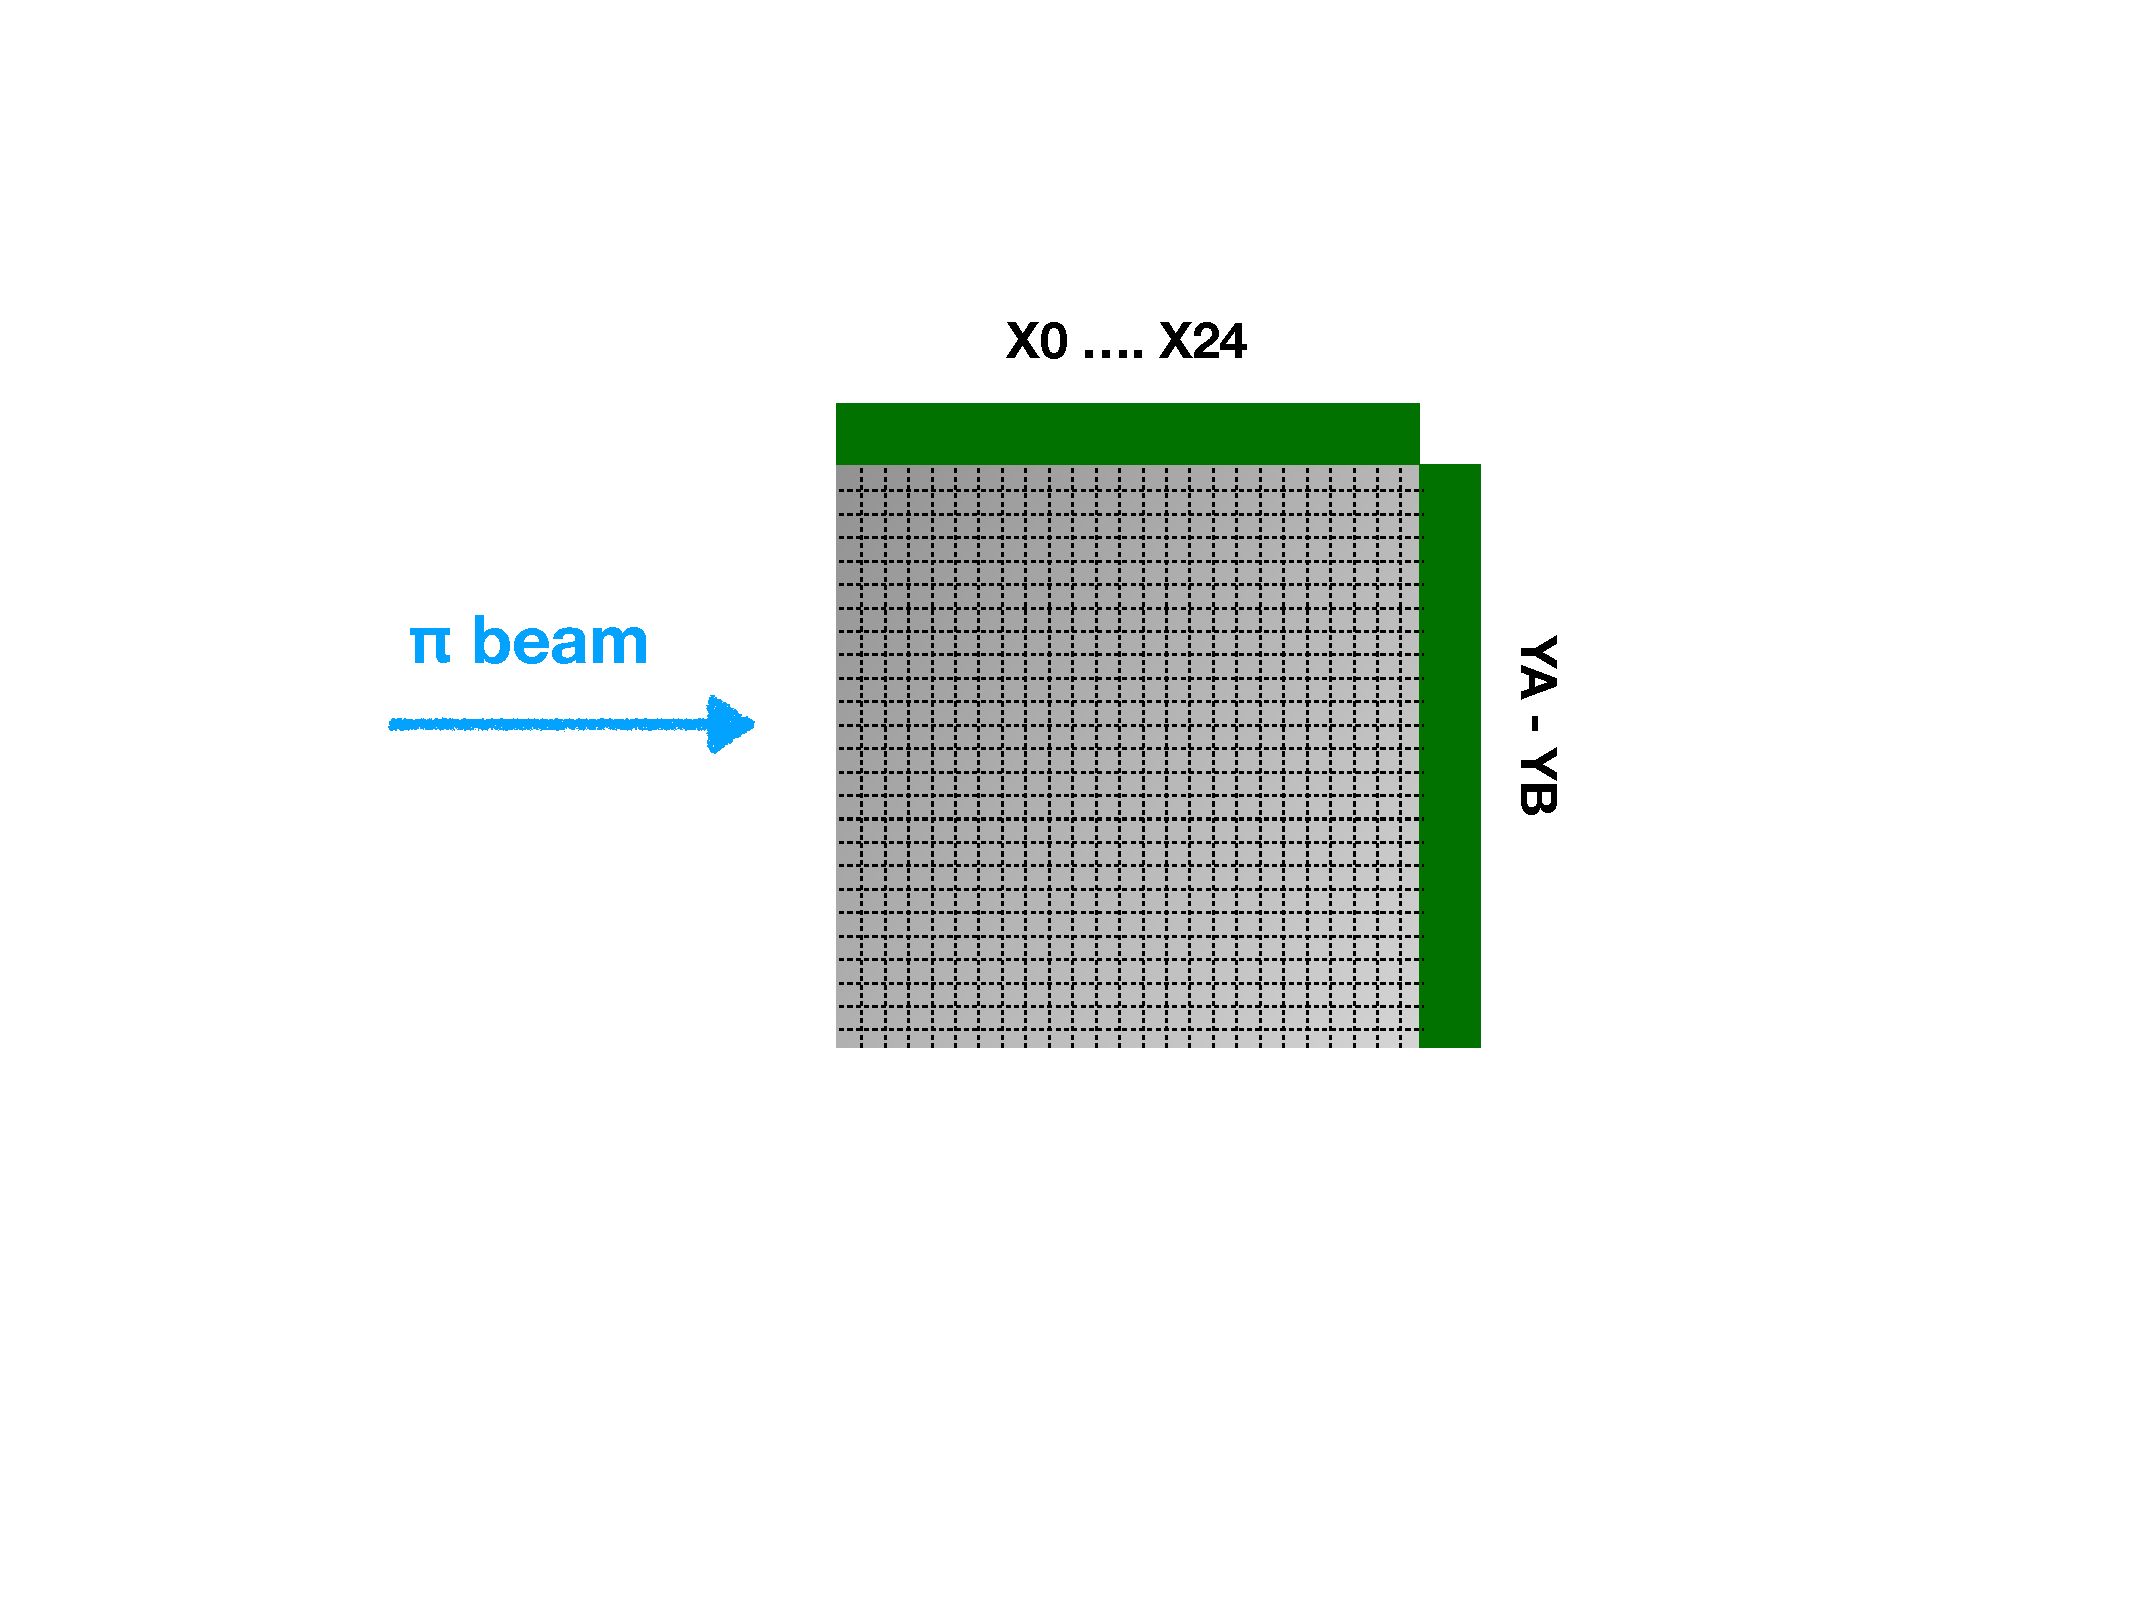
\includegraphics[width=\textwidth]{xcal.pdf}
	\caption{x-side}\label{mipx}
	\end{subfigure}
	\begin{subfigure}[b]{0.29\textwidth}
	\centering
	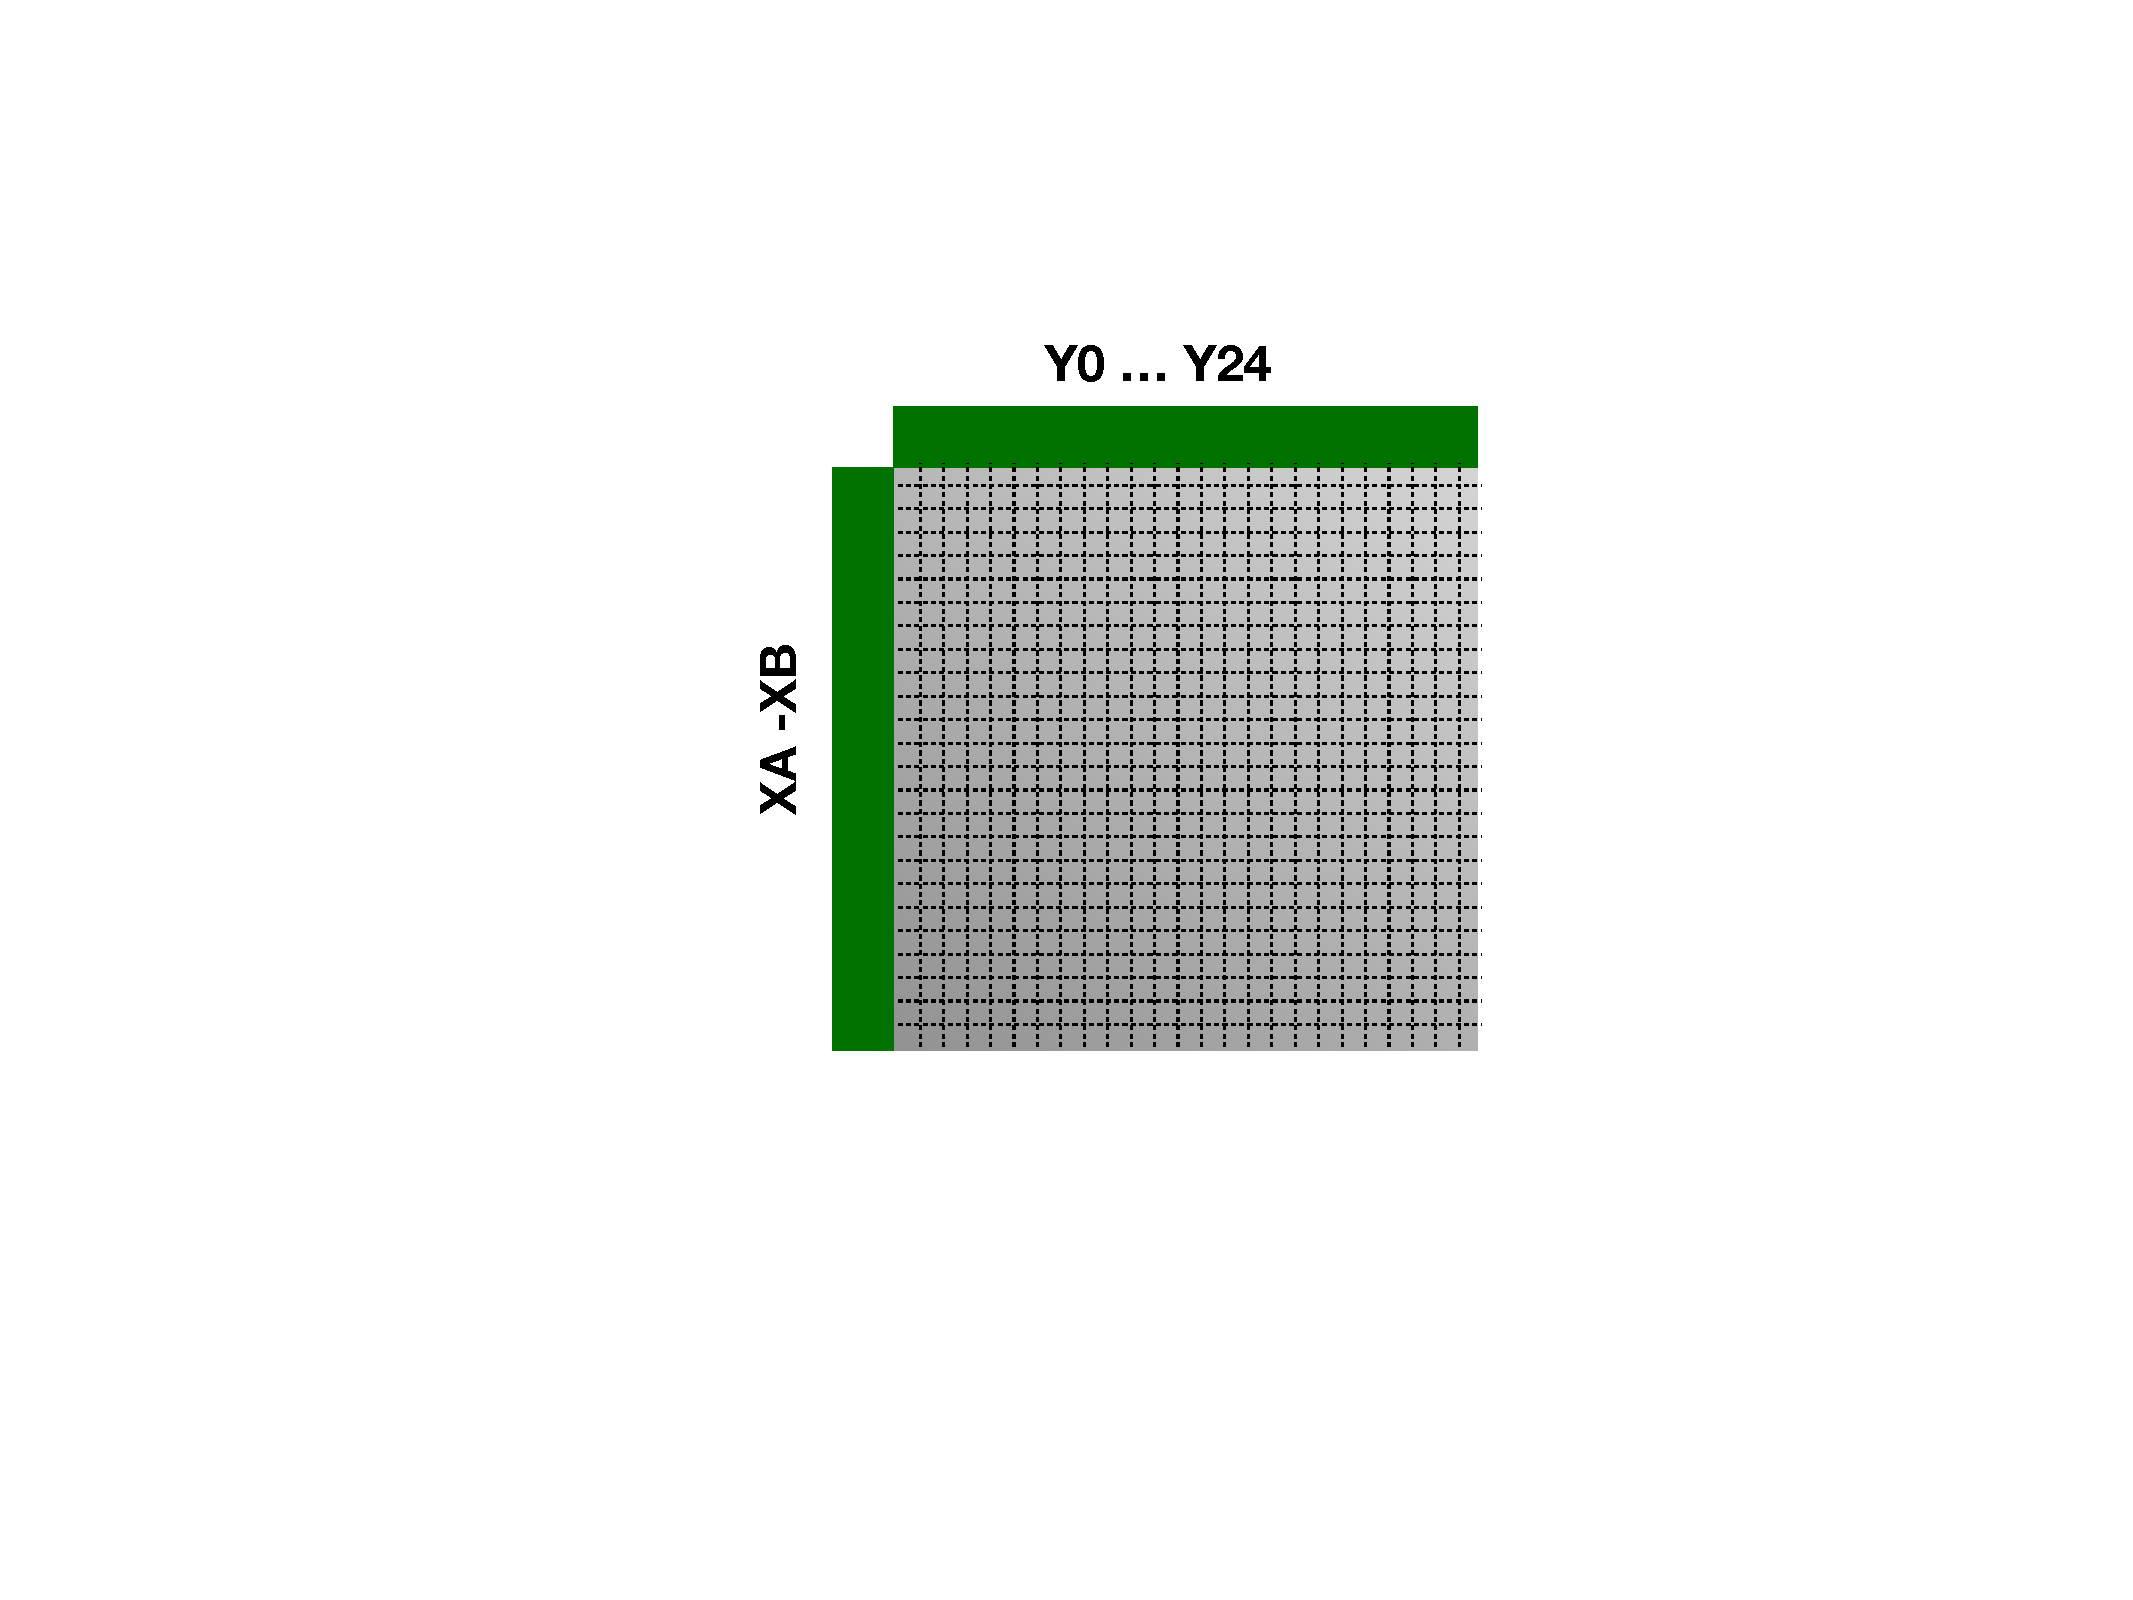
\includegraphics[width=\textwidth]{ycal.pdf}
	\caption{y-side}\label{mipy}
	\end{subfigure}
	\begin{subfigure}[b]{0.14\textwidth}
	\centering
	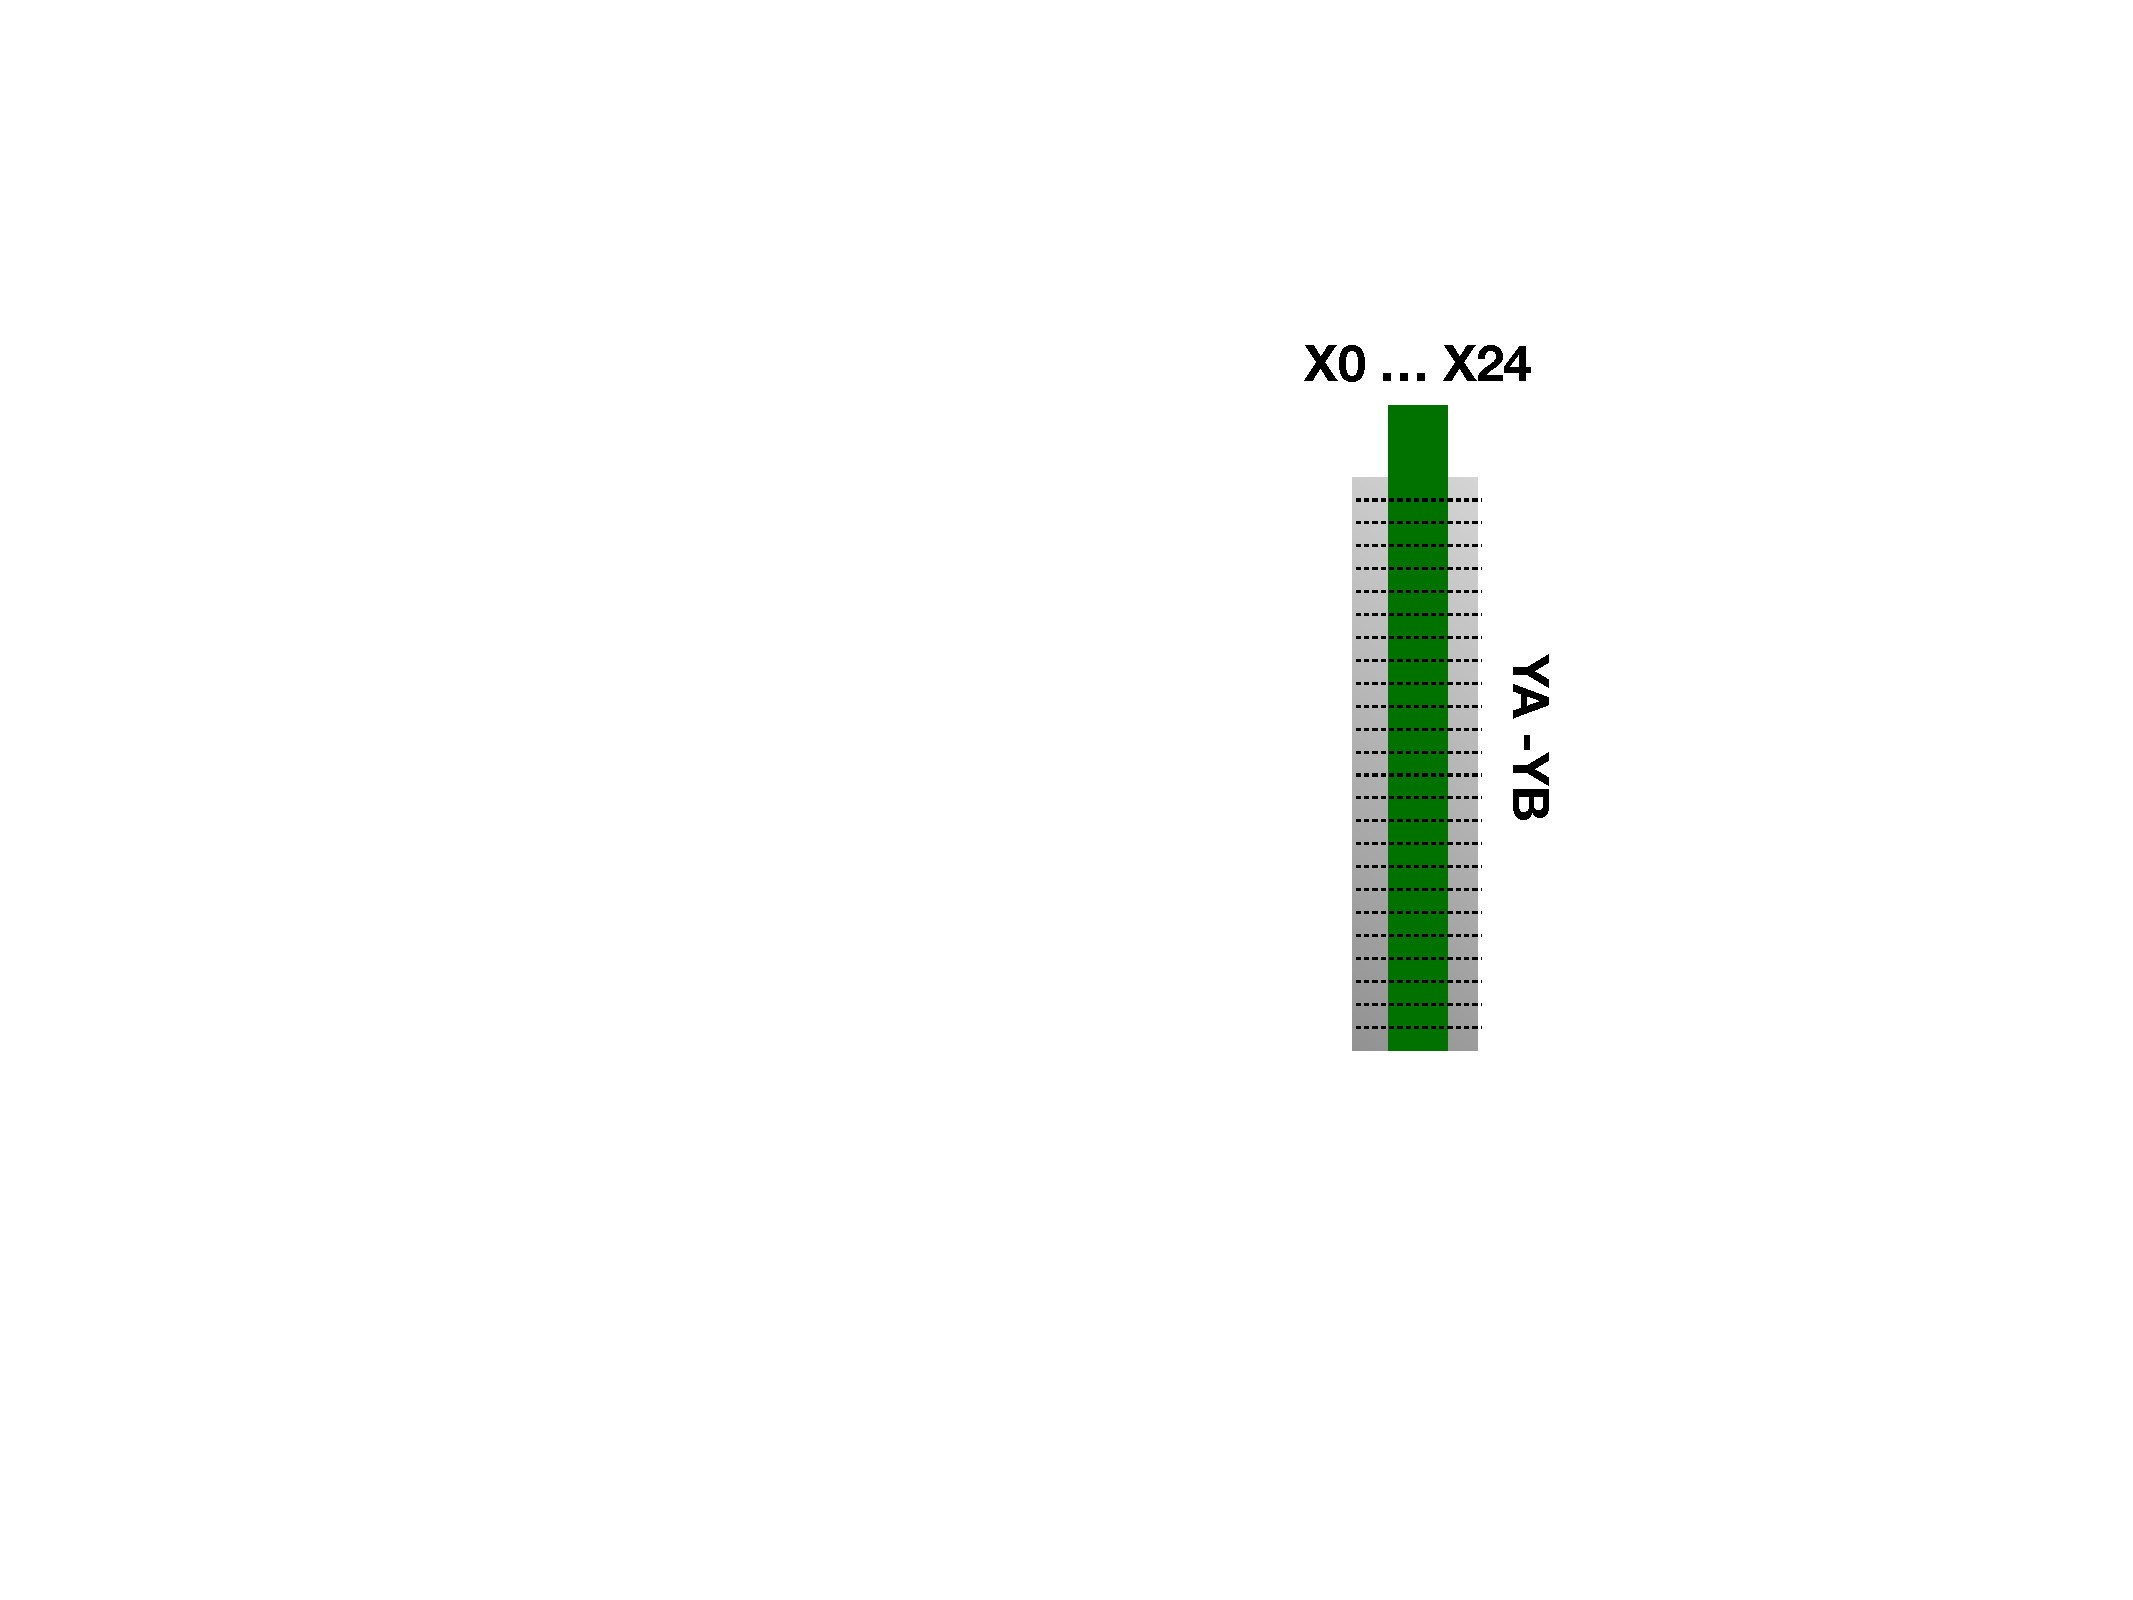
\includegraphics[width=\textwidth]{zcal.pdf}
	\caption{z-side}\label{mipz}
	\end{subfigure}\hspace*{\fill}
	\caption{Detector position for calibration. Pion beam is always from the left to the right on the three configurations}\label{mip}
\end{figure}

With a program COOOL designed for monitoring events online (see Figure\ref{coool}), it was possible to look at the histograms were shows the total
amplitude register on each channel removing the pedestal. The first spills shows us a Vavilov-Landau distribution on the
histograms with a peak value around 20-50 a.u. depending on the channel. Thereafter the bias voltage on the 5 shared channels
were adjusted to obtain a considerable same peak value. The range of the voltage for the MPPC goes from
\SIrange{68}{72}{V} therefore, a peak value of around 75 a.u. respect to pedestal was the goal. Once the equalizations is achieved a new run
is performed with few spills with enough events to perform the calibration offline.\par 

\begin{figure}[ht]
	\hspace*{\fill}
	\centering
	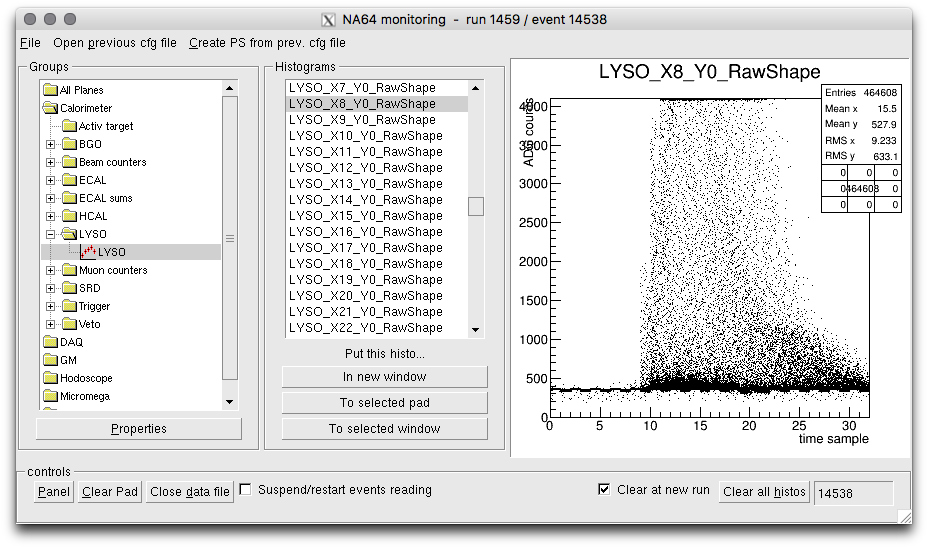
\includegraphics[width=0.8\textwidth]{COOOL.png}
	\hspace*{\fill}
	\caption{Monitoring application COOOL showing a waveform from channel x8. 32 time samples are obtaine from the two
	ADC and 4096 channels for amplitude counts. Pedestal around 400 ADC counts}\label{coool}
\end{figure}

\begin{equation}\label{wave}
\mathrm{wave}_{i}=\left\{a_0,a_1,\dotsc,a_{30},a_{31}\right\}
\end{equation}

The {\bf Run 1459} with 10 spills ($\sim$70k events) it is enough to perform the calculations for pedestal position and
width. The raw data is a digitized pulse of 32 time samples \ref{rawpulse}, with one sample each \SI{12}{ns} thanks to the
combination of two ADC's.

\begin{figure}[ht]
	\hspace*{\fill}
	\centering
	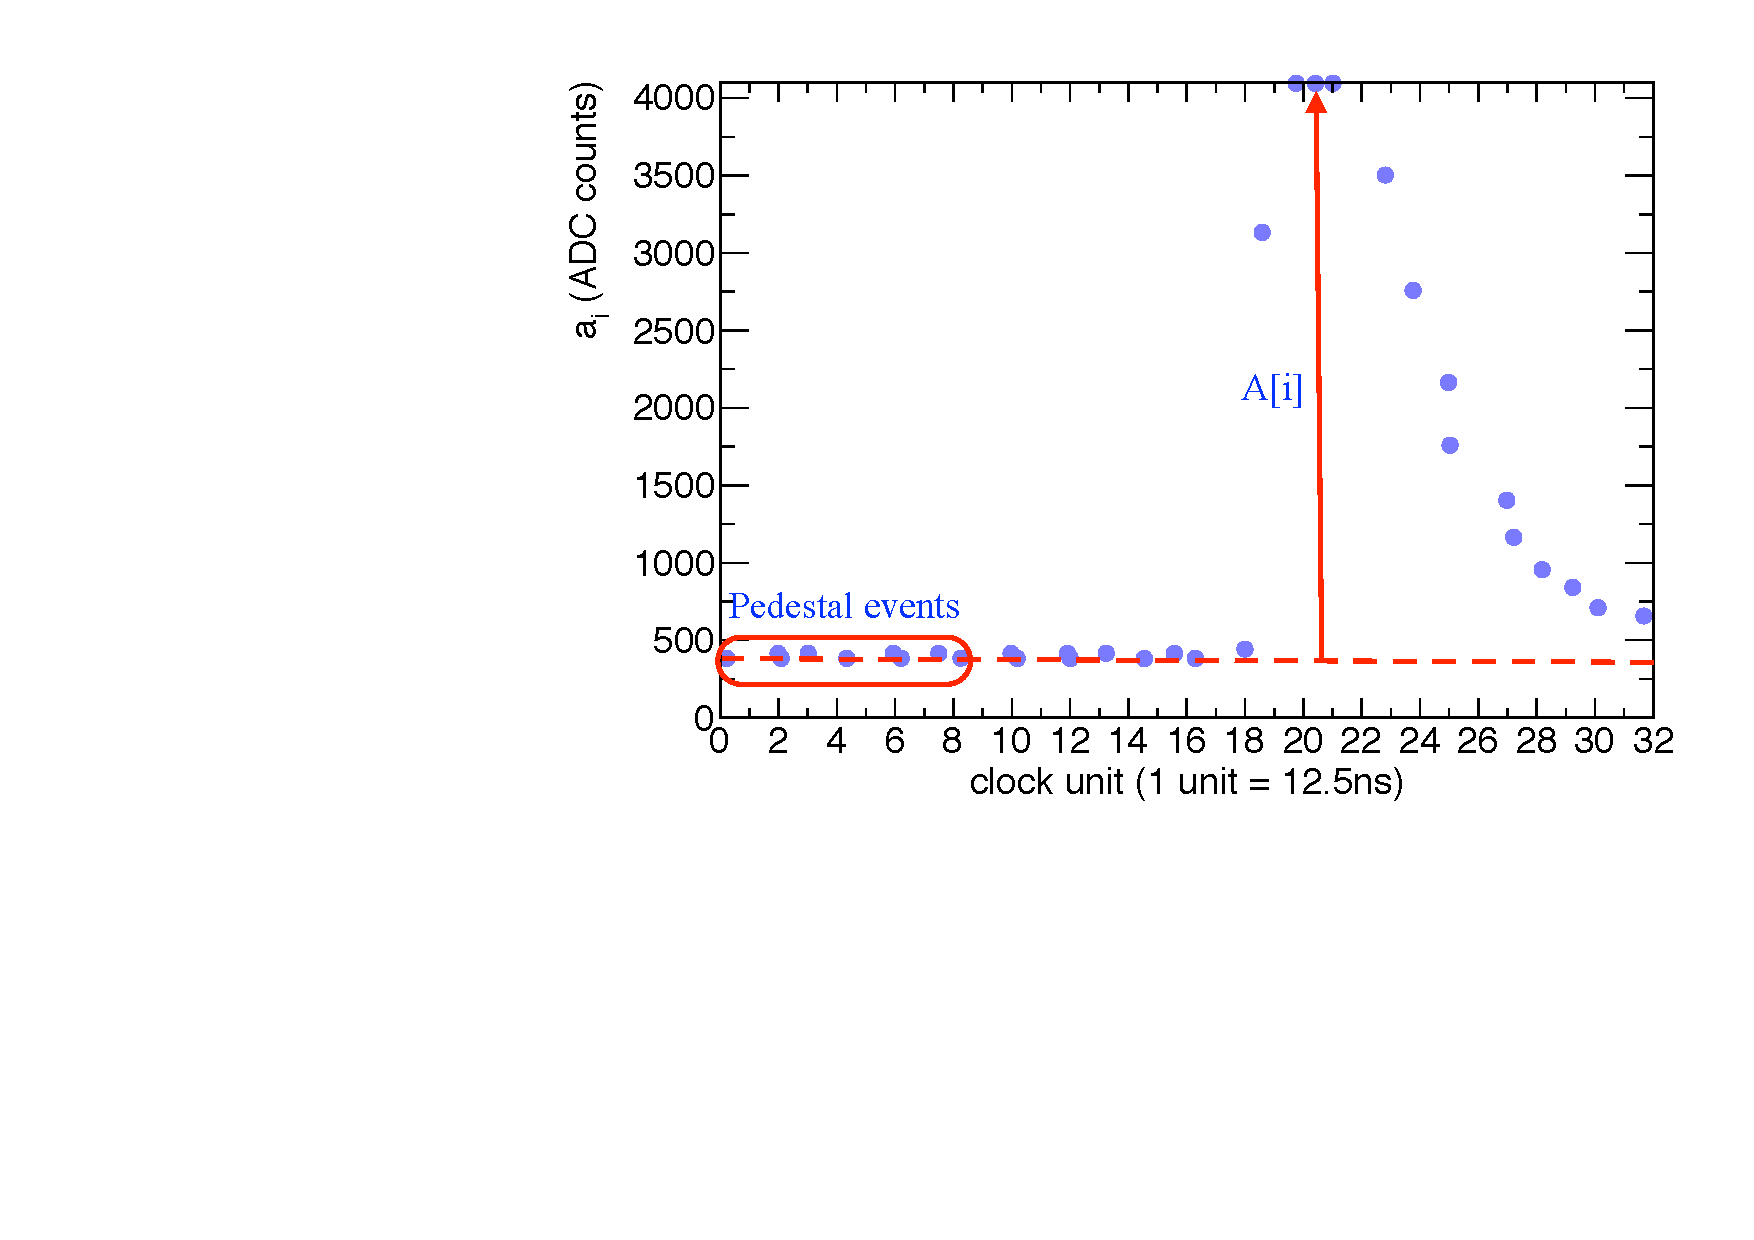
\includegraphics[width=0.5\textwidth]{wave_sample.pdf}
	\hspace*{\fill}
	\caption{}\label{}
\end{figure}

\begin{equation}\label{pedeqn}
\mathrm{ped}0=\frac{1}{4}\sum_{i=0,2,4,6}a_i \qquad \mathrm{ped}1=\frac{1}{4}\sum_{i=1,3,5,7}a_i
\end{equation}

Two pedestal are calculated from the first 8 time samples according to equation \ref{pedeqn} from the wave.
Afterwards, the pedestal is subtracted from the wave eqn.\ref{wave} according to the position (odd or even)

\begin{equation}\label{waveped}
\overline{\mathrm{wave}}_{i}=\left\{a_0-\mathrm{ped}0,a_1-\mathrm{ped}1,\dotsc,a_{30}-\mathrm{ped}0,a_{31}-\mathrm{ped}1\right\}
\end{equation}

For analysis purpose, an estimation of the pedestal signal is performed as the average of ped0 and ped1. The monitoring
program COOOL shows the pedestal while the data taking is running and an example of it is shown in Figure
\ref{pedestal}. However, a full analysis of the pedestal is performed offline. For each channel an histogram for pedestal
is calculated with the average of ped0 and ped1 per triggered event. A Gaussian fit is applied to the pedestal signal
and the parameter $\mu$ and $\sigma$ are shown in Figure \ref{pedsum}.

\begin{figure}[ht]
	\hspace*{\fill}
	\begin{subfigure}[b]{0.4\textwidth}
	\centering
	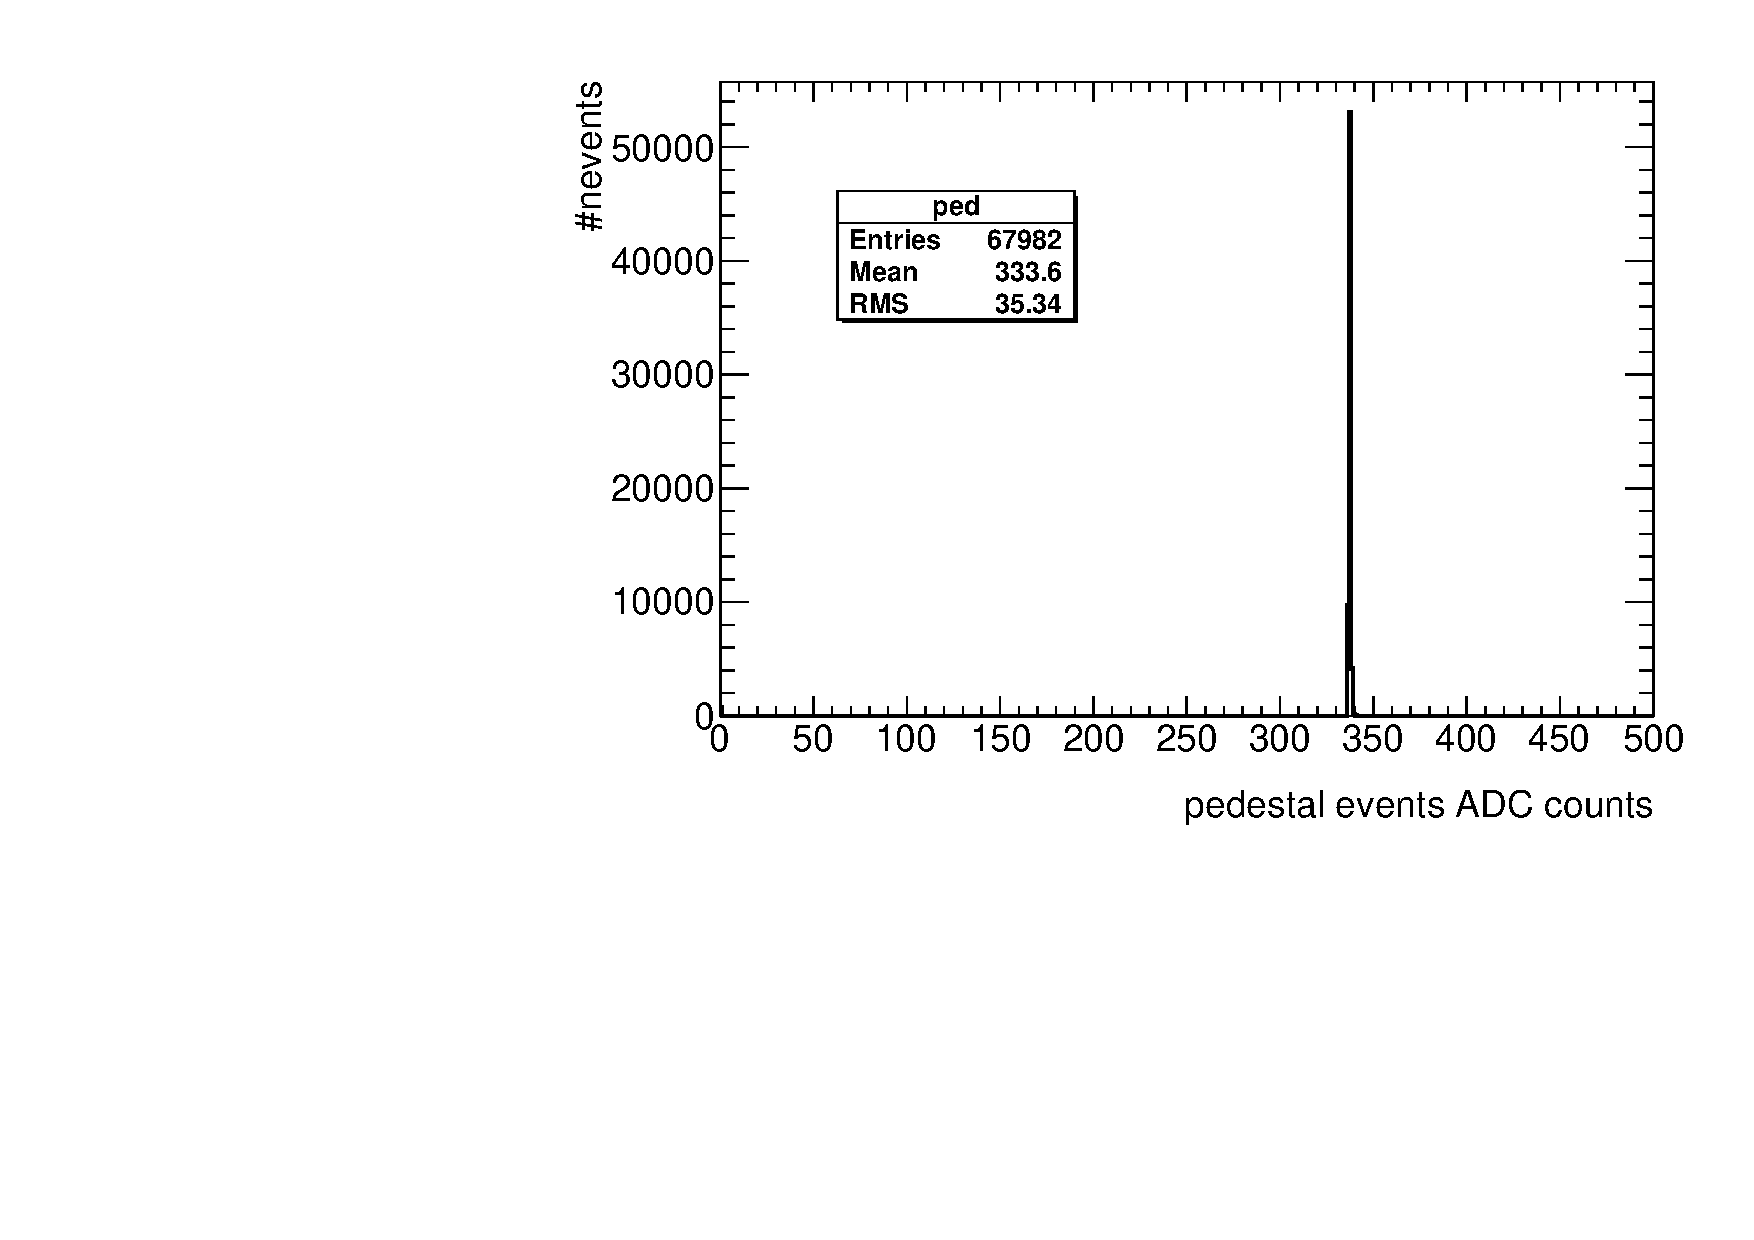
\includegraphics[width=\textwidth]{ped_sample.pdf}
	\caption{Pedestal example from COOOL. $\sim$ 1 ADC count as RMS}\label{pedestal}
	\end{subfigure}
	\begin{subfigure}[b]{0.4\textwidth}
	\centering
	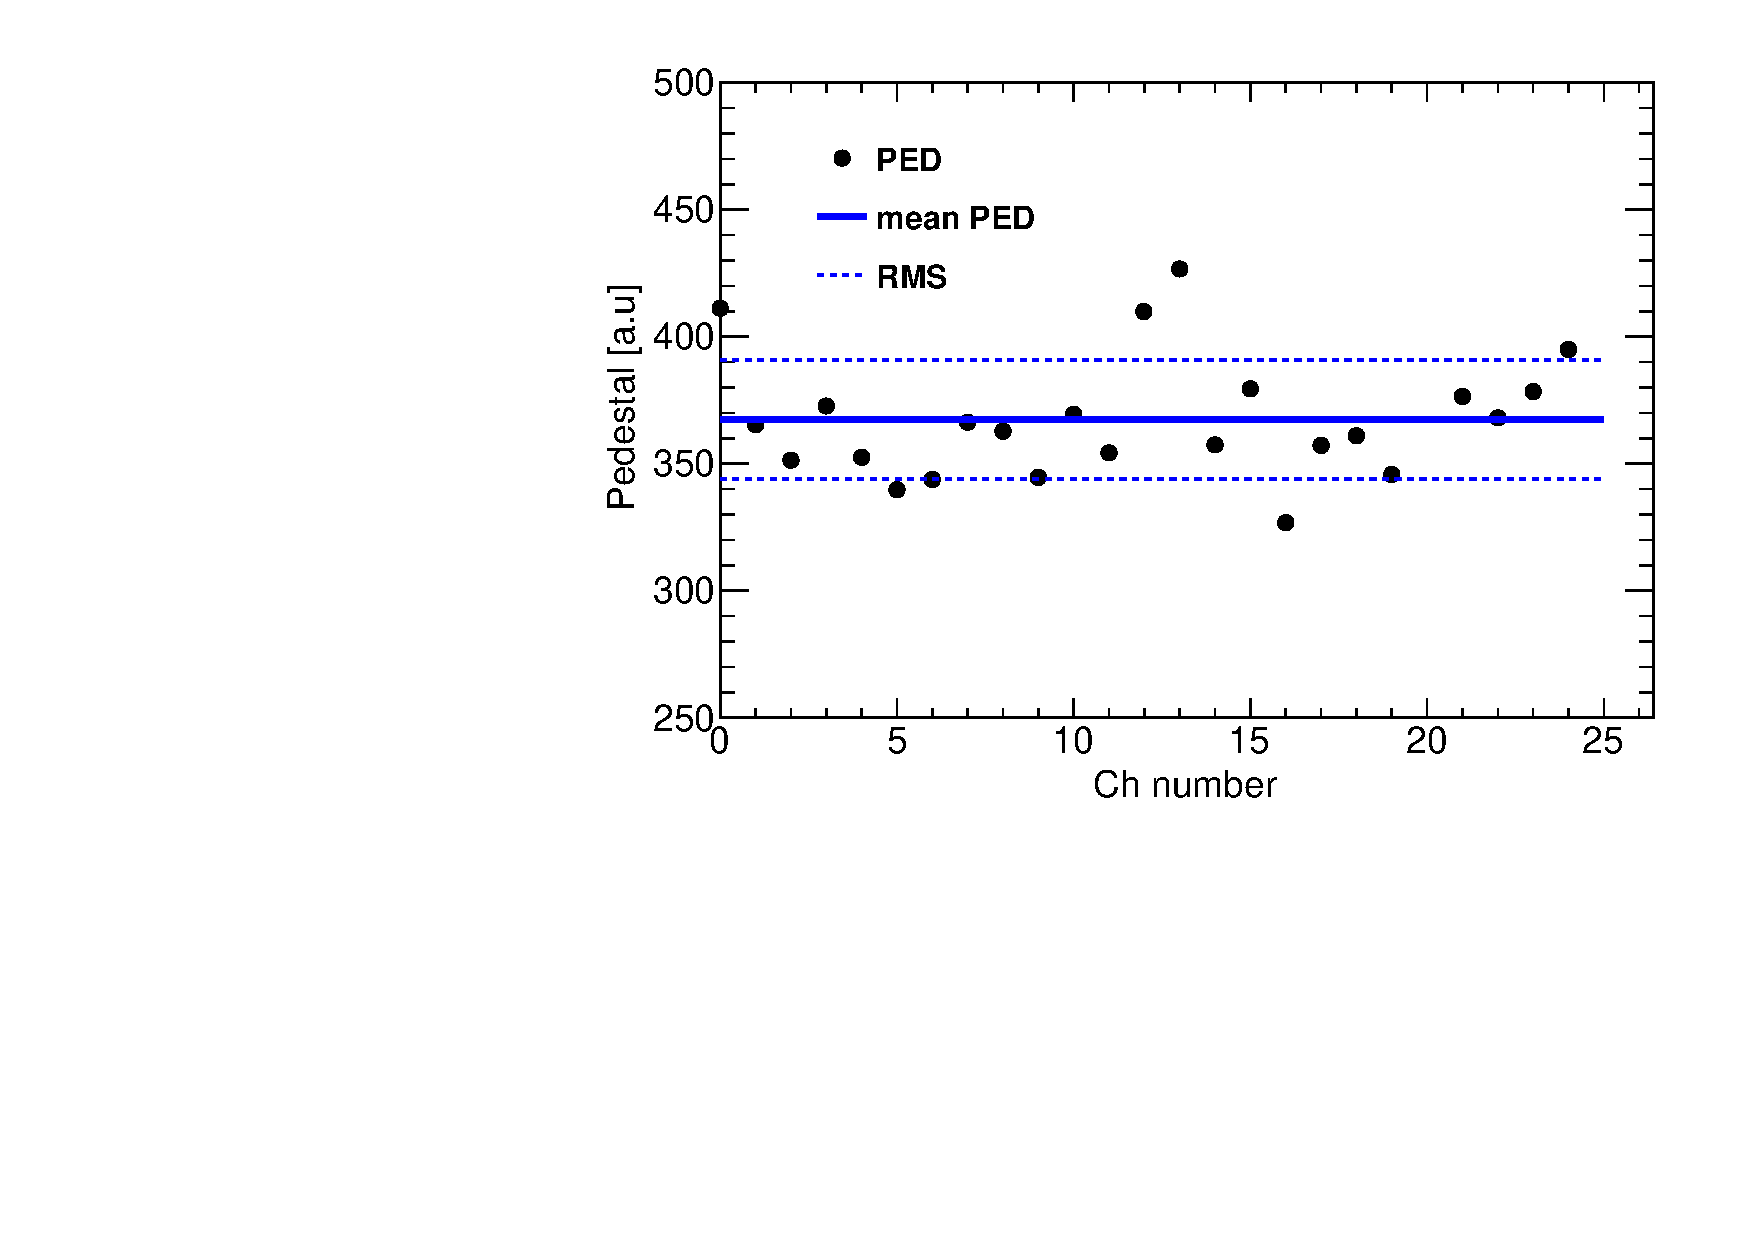
\includegraphics[width=\textwidth]{pedx.pdf}
	\caption{Pedestal summary for each channel, calculated offline. A Gaussian fit is performed for each channel where a
	$\sigma\sim 1$ is obtained in all of them.}\label{pedsum}
	\end{subfigure}
	\hspace*{\fill}
	\caption{Pedestal summary}\label{}
\end{figure}

A summary of pedestal of each channel on x-axis is presented in Figure \ref{pedsum}. The data set represent the $\mu$
parameter from a Gaussian distribution, and where $\sigma\sim 1$ for each channel. The graph also show the avarage
pedestal around 365 for all channels and the RMS of about 25, which highlight the stability of the system and the detector.\par

\begin{figure}[ht]
	\hspace*{\fill}
	\centering
	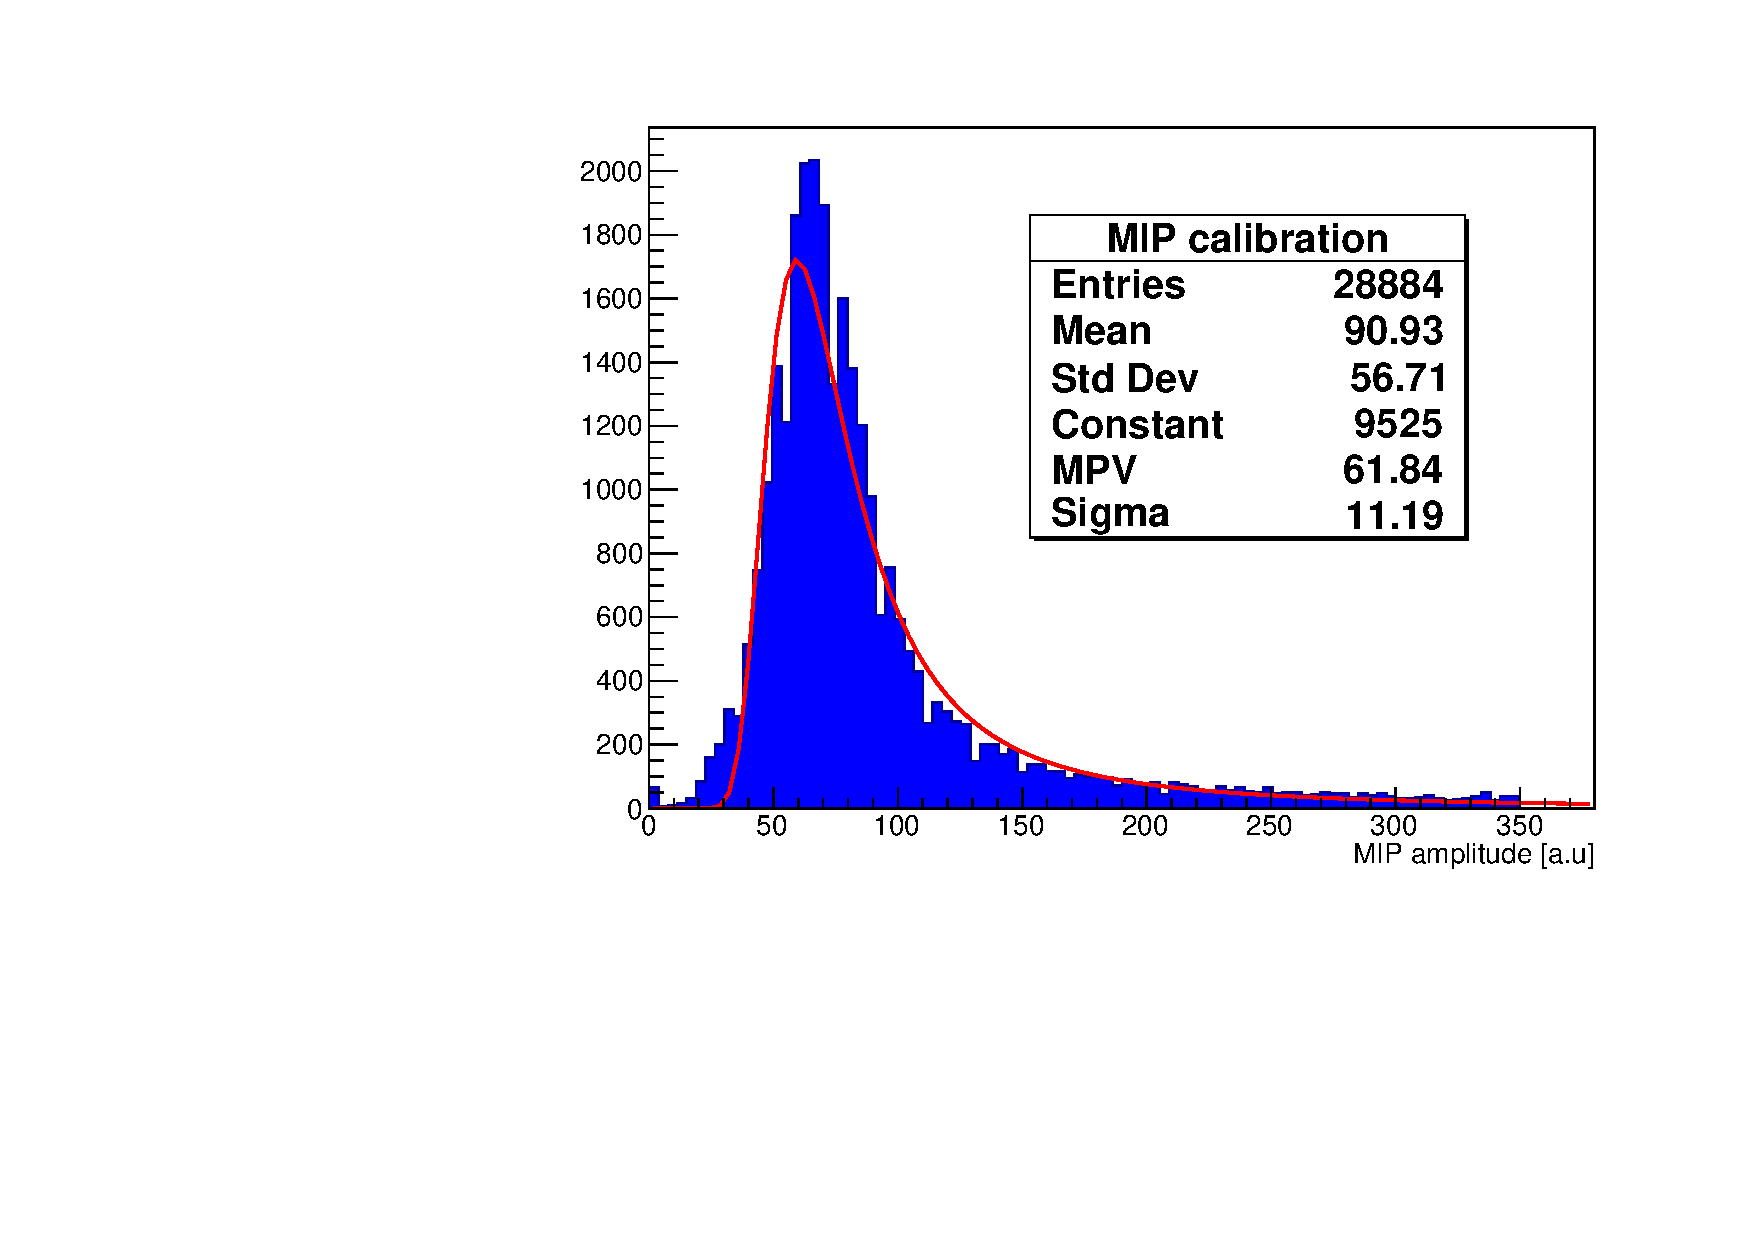
\includegraphics[width=0.5\textwidth]{mip_onech.pdf}
	\hspace*{\fill}
	\caption{Histogram from amplitude when a MIP pass through the crystal across \SI{0.4}{cm}}\label{landau}
\end{figure}

The ADC integrate the analog pulse from the detector and then goes to a shaper pulse to deliver the waveform from Figure
\ref{coool}. The maximum of this pulse gives the charge integrated from the analog pulse, therefore an histogram with
the maximum amplitude will be proportional to the amount of energy deposited by an ionization. \par To estimate the
energy on the detector, a comparison between the most probable value (MPV) from a Landau fit and the energy loss on a
small thickness material is performed. Such way each MPV from each channel can be compare to the 5.68MeV and the obtain
the calibrations factors for each channel. The Figure \ref{landau} shows an example from this method, where a Landau fit
is performed (red line) and it also shows the MIP value (\SI{5.68}{MeV}) is relative close to the pedestal (a value 0 in the
histogram) since the peak expected from SR is around 11MeV. However the separation from the peak value is enough to see
the Landau distribution start from 0 counts aroun 5a.u.\par


\begin{figure}[ht]
	\hspace*{\fill}
	\centering
		\begin{subfigure}[b]{0.45\textwidth}
			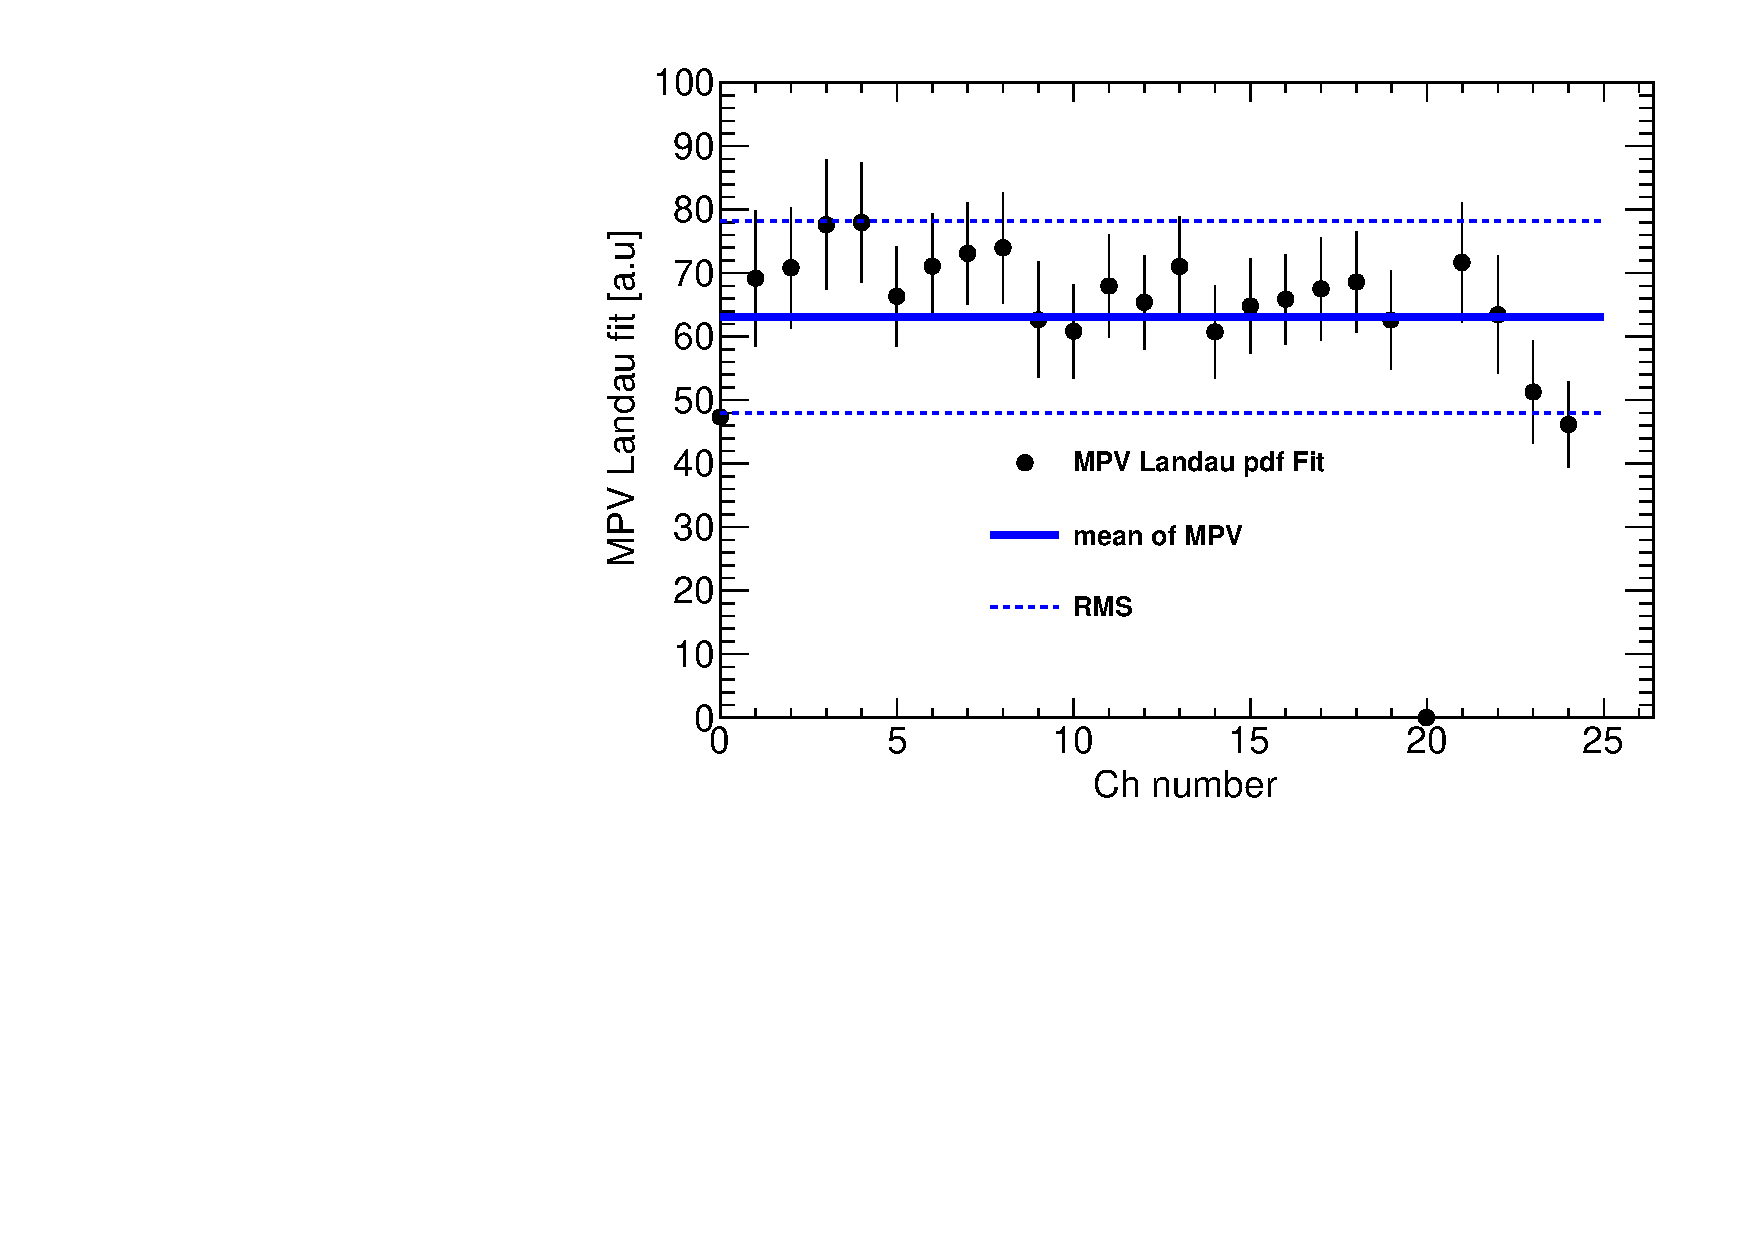
\includegraphics[width=\textwidth]{mpvx.pdf}
			\caption{Mip position on x-side}\label{gainx}
		\end{subfigure}
		\hfill
		\begin{subfigure}[b]{0.45\textwidth}
			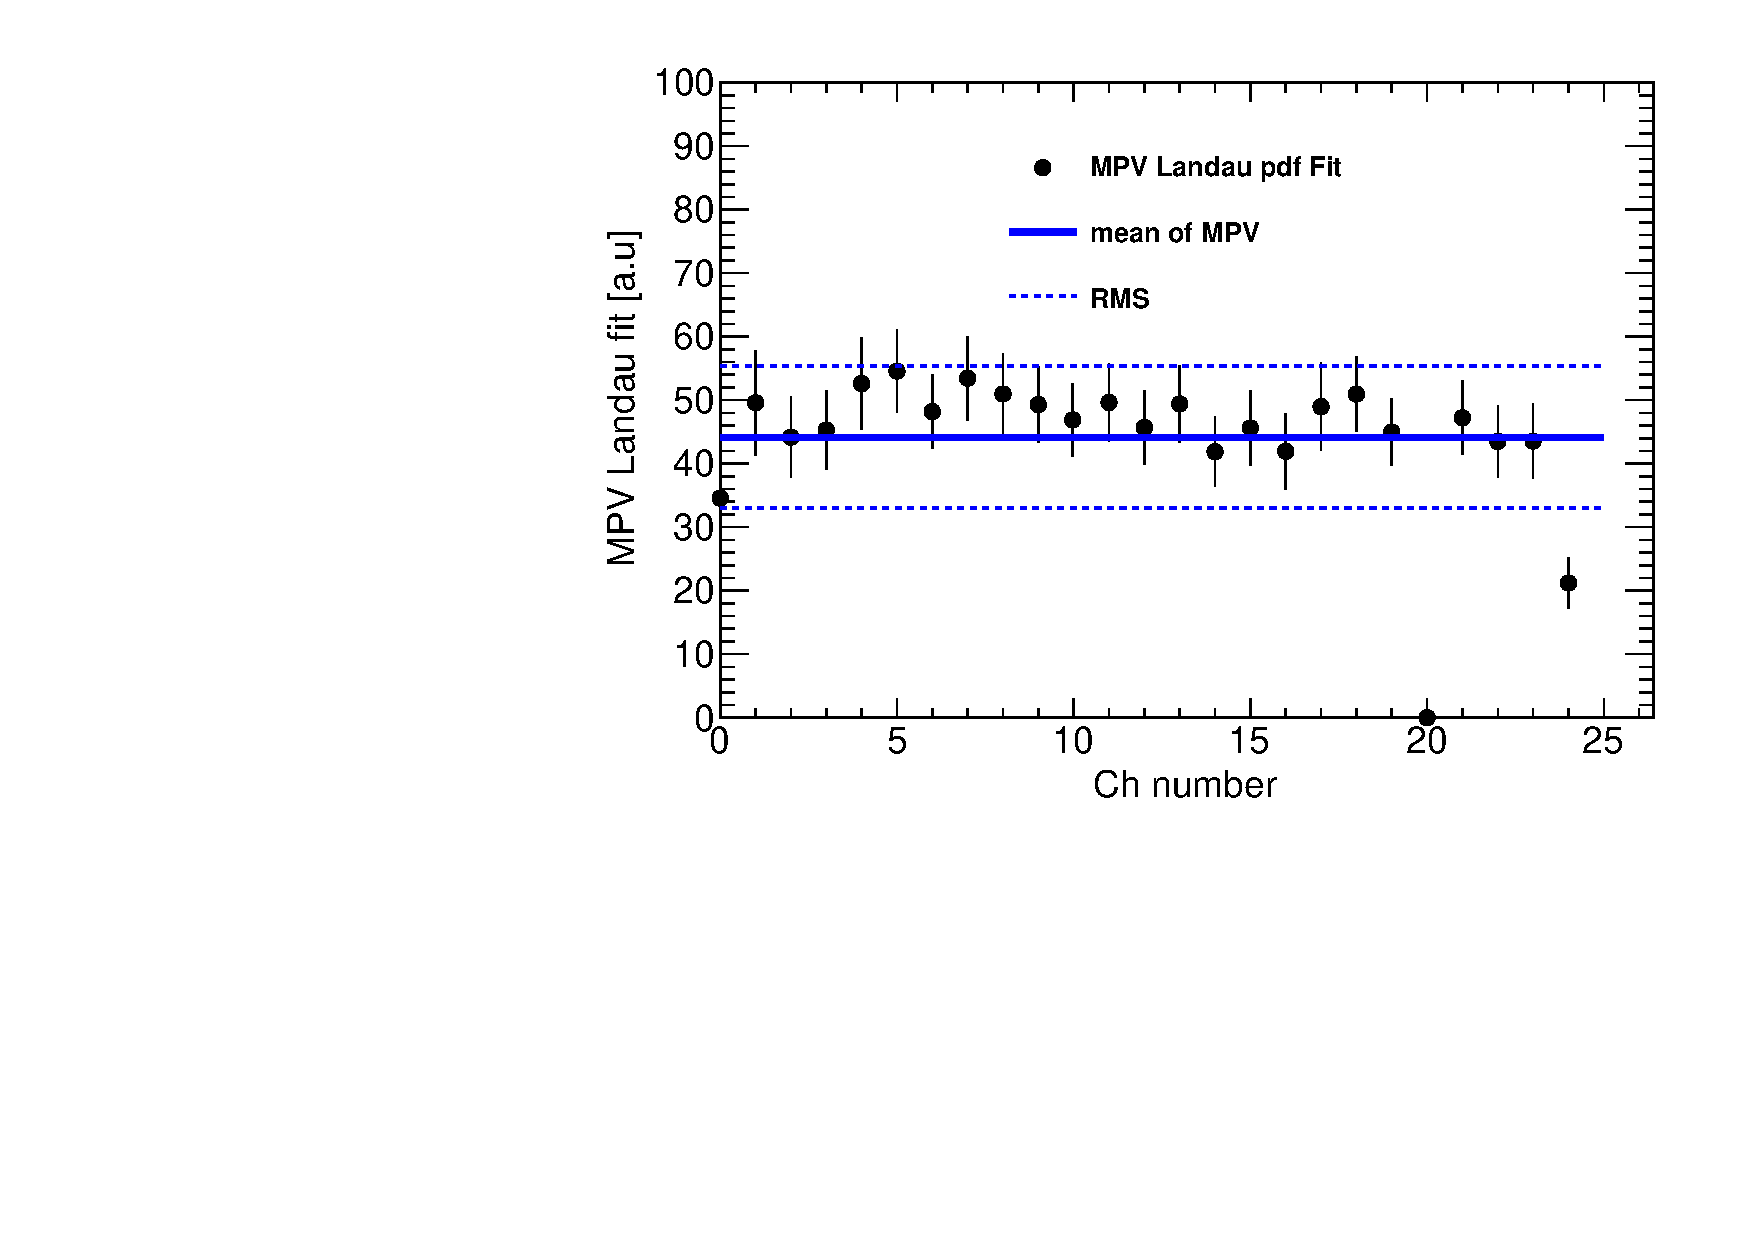
\includegraphics[width=\textwidth]{mpvy.pdf}
			\caption{Mip position y-side}\label{gainy}
		\end{subfigure}
\hspace*{\fill}
	\caption{Gain equalization. Data sets excluding channel 20 for high pedestal and shape problems.}\label{equalization}
\end{figure}

One set of data (run 1459) was taken with the configuration {\bf(a)} on Figure \ref{mip} where a pion beam hits at least
one crystal per channel on the x-side. Afterwards the MIP position is identified and estimated the most probable value
(MPV) for each channel. A graph who summarize this procedure is shown in Figure \ref{gainx}. Afterwards, the detector is
turn over and the electronic boards are swapped to observe each channel on the y-side. Then a 10 spills {\bf run 1463} is
recorded and the MIP position is adjusted on each channel to 50a.u. above pedestal. The reason for this number is the
maximum ADC count is app 4000 units, and if all the channel provide a signal we will get an overflow on the two weighted
signals.\par The MIP position for the y-side is shown in Figure\ref{gainy} with an average of 45 a.u.. Both graph shows
a MPV=0 para ch number 20, that is because that channel has a high pedestal ($\sim$ 3000 ADC counts) and it was remove
from all the analysis. The Figure \ref{badch} shows the pulse from channel 20 which clearly expose a bipolar pulse. \par

\begin{figure}[ht]
	\hspace*{\fill}
	\centering
	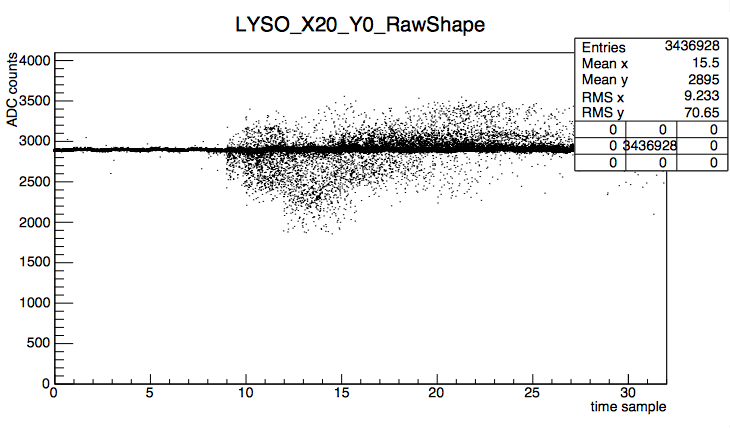
\includegraphics[width=0.6\textwidth]{badch.png}
	\hspace*{\fill}
	\caption{Bad channel}\label{badch}
\end{figure}

In the configuration {\bf (c)}, when the detector is perpendicular to the beam (Figure\ref{mipz}), the mean energy
deposited by a minimum ionizing particle is $E_{\mathrm{mip}}\sim 64$MeV. It means for every event, the total light
collected should be proportional to $E_{\mathrm{mip}}$. The Figure \ref{sumx} correspond to the run 1467, a pion beam,
and shows the amount of energy deposited on the LYSO detector. The total amount of energy is calculated as:
\begin{equation}
E=\sum_{ch=0}^{24} a[ch]*c_0[ch]
\end{equation}
where $c_0$ correspond to the calibration coefficients calculated as $c_0[ch]=5.68/\mathrm{MPV}[ch]$ and $a[ch]$
correspond to the max amplitude per ch on each event.\par


\begin{figure}[ht]
	\hspace*{\fill}
	\centering
	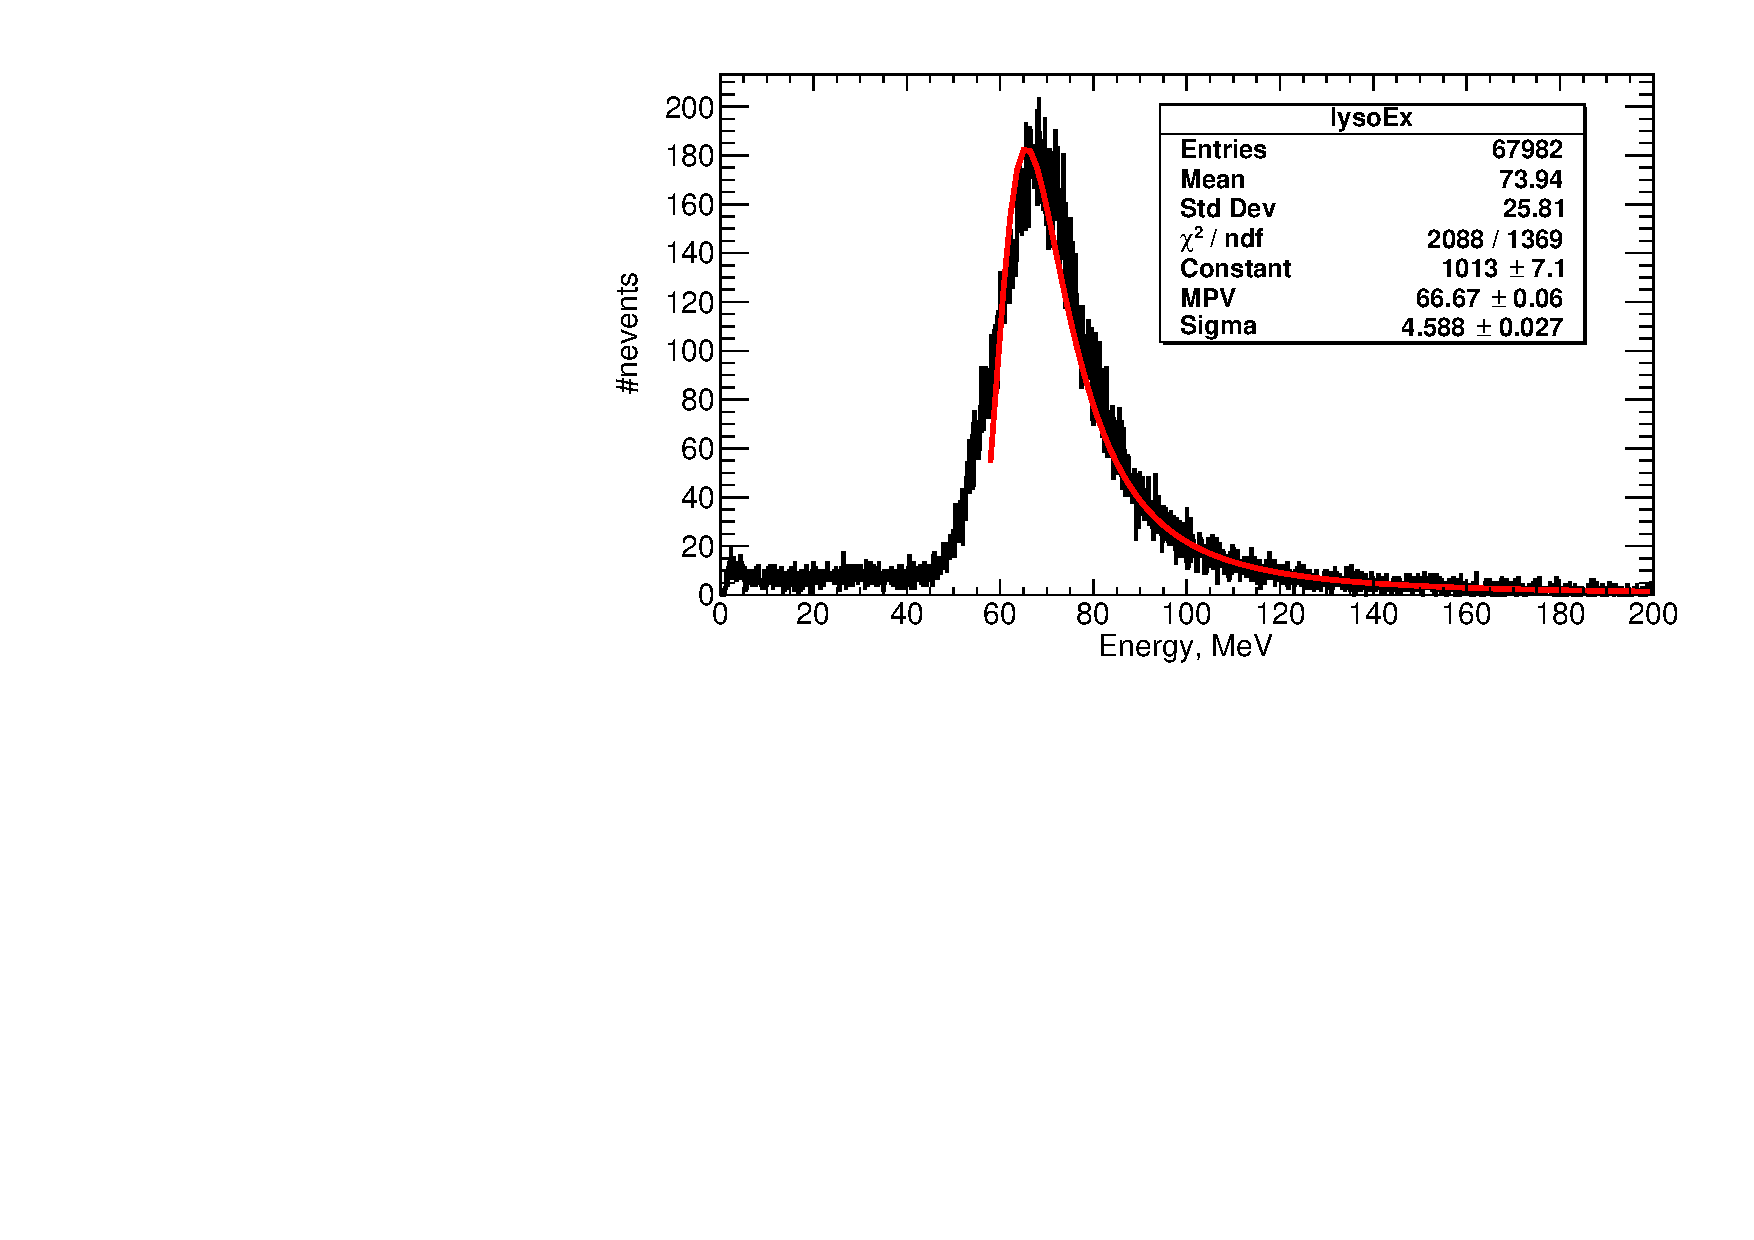
\includegraphics[width=0.6\textwidth]{sumx.pdf}
	\hspace*{\fill}
	\caption{Sum of every channel amplitude with the calibration coefficient provided in ref{}}\label{sumx}
\end{figure}

A Landau fit is applied to total energy deposited on x-side, and a 66MeV as MPV is obtained compare to the 64MeV
expected. To estimate the energy resolution, the parameter $\xi$ from a Landau pdf is used as sigma and the
resolution is estimated by full width at half maximum (FWHM) where the maximum correspond to the MPV on the Landau pdf. 
\begin{equation}
\mathrm{FWHM} = 2.355 \sigma
\end{equation}
Where for the x-side gives a Resolution of : $2.355*4.588/66.67=16\%$, early reported on \ref{datasheetLYSO} a $8\%$ of
energy resolution of one crystal at 662keV.\par

On the y-side, every channel was equalized to around the same MPV value (50 ADC counts). Therefore, both weighted signal
should show the same distribution with slightly same MPV values. The Figure \ref{y_signals} shows a Landau pdf for each
weighted signal $Y_A$ and $Y_B$ since both are the sum over all channels with some gain factors.\par

Applying a Landau fit over the sum of both $YA$ and $YB$ amplitudes, we can estimate the resolution for the y-axis.
The Figure \ref{y_sumab} shows the histogram of both weighted signal with a Landau fit. With a MPV of 1207 (ADC counts)
and a $\xi=89.5$ results in a $17\%$ energy resolution at 64MeV.\par 

\begin{figure}[ht]
	\hspace*{\fill}
	\centering
		\begin{subfigure}[b]{0.45\textwidth}
			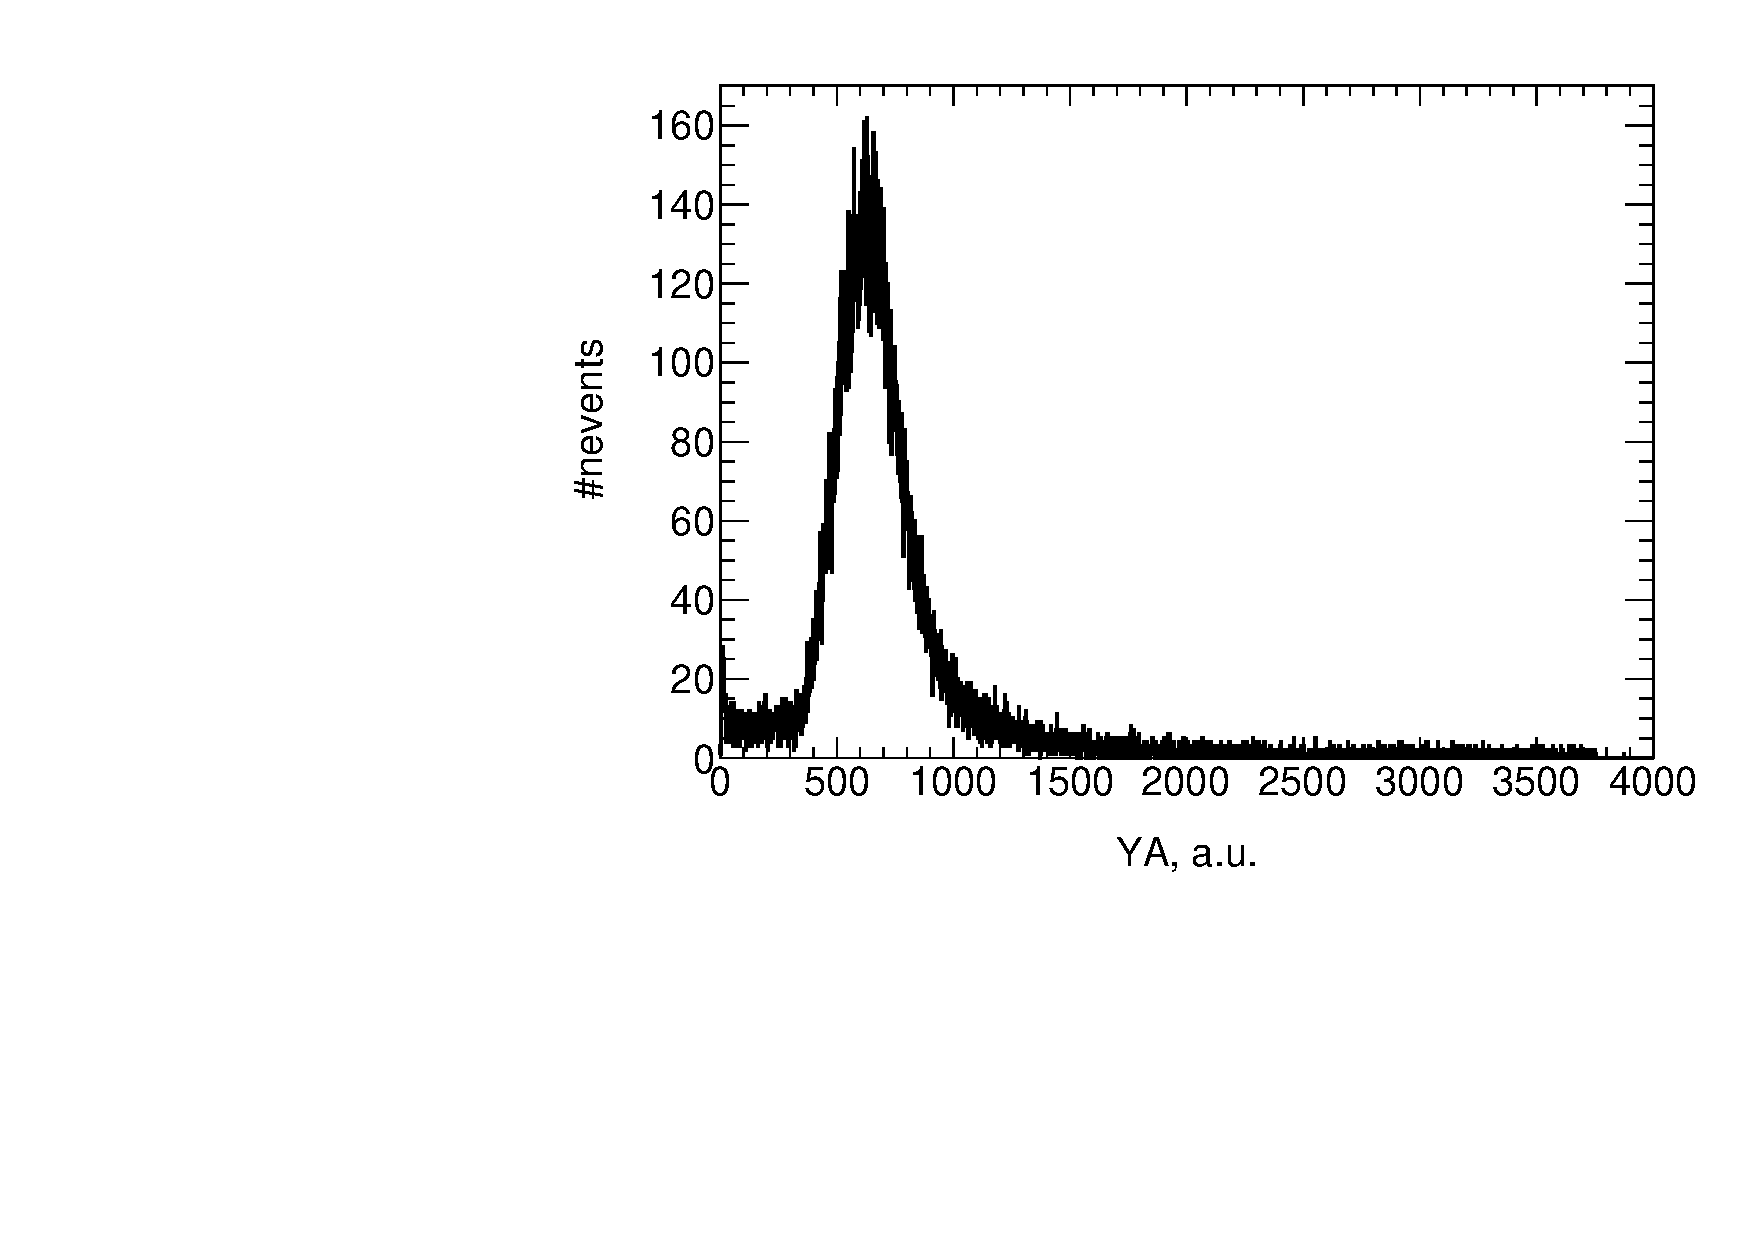
\includegraphics[width=\textwidth]{ya.pdf}
			\caption{}\label{}
		\end{subfigure}
		\hfill
		\begin{subfigure}[b]{0.45\textwidth}
			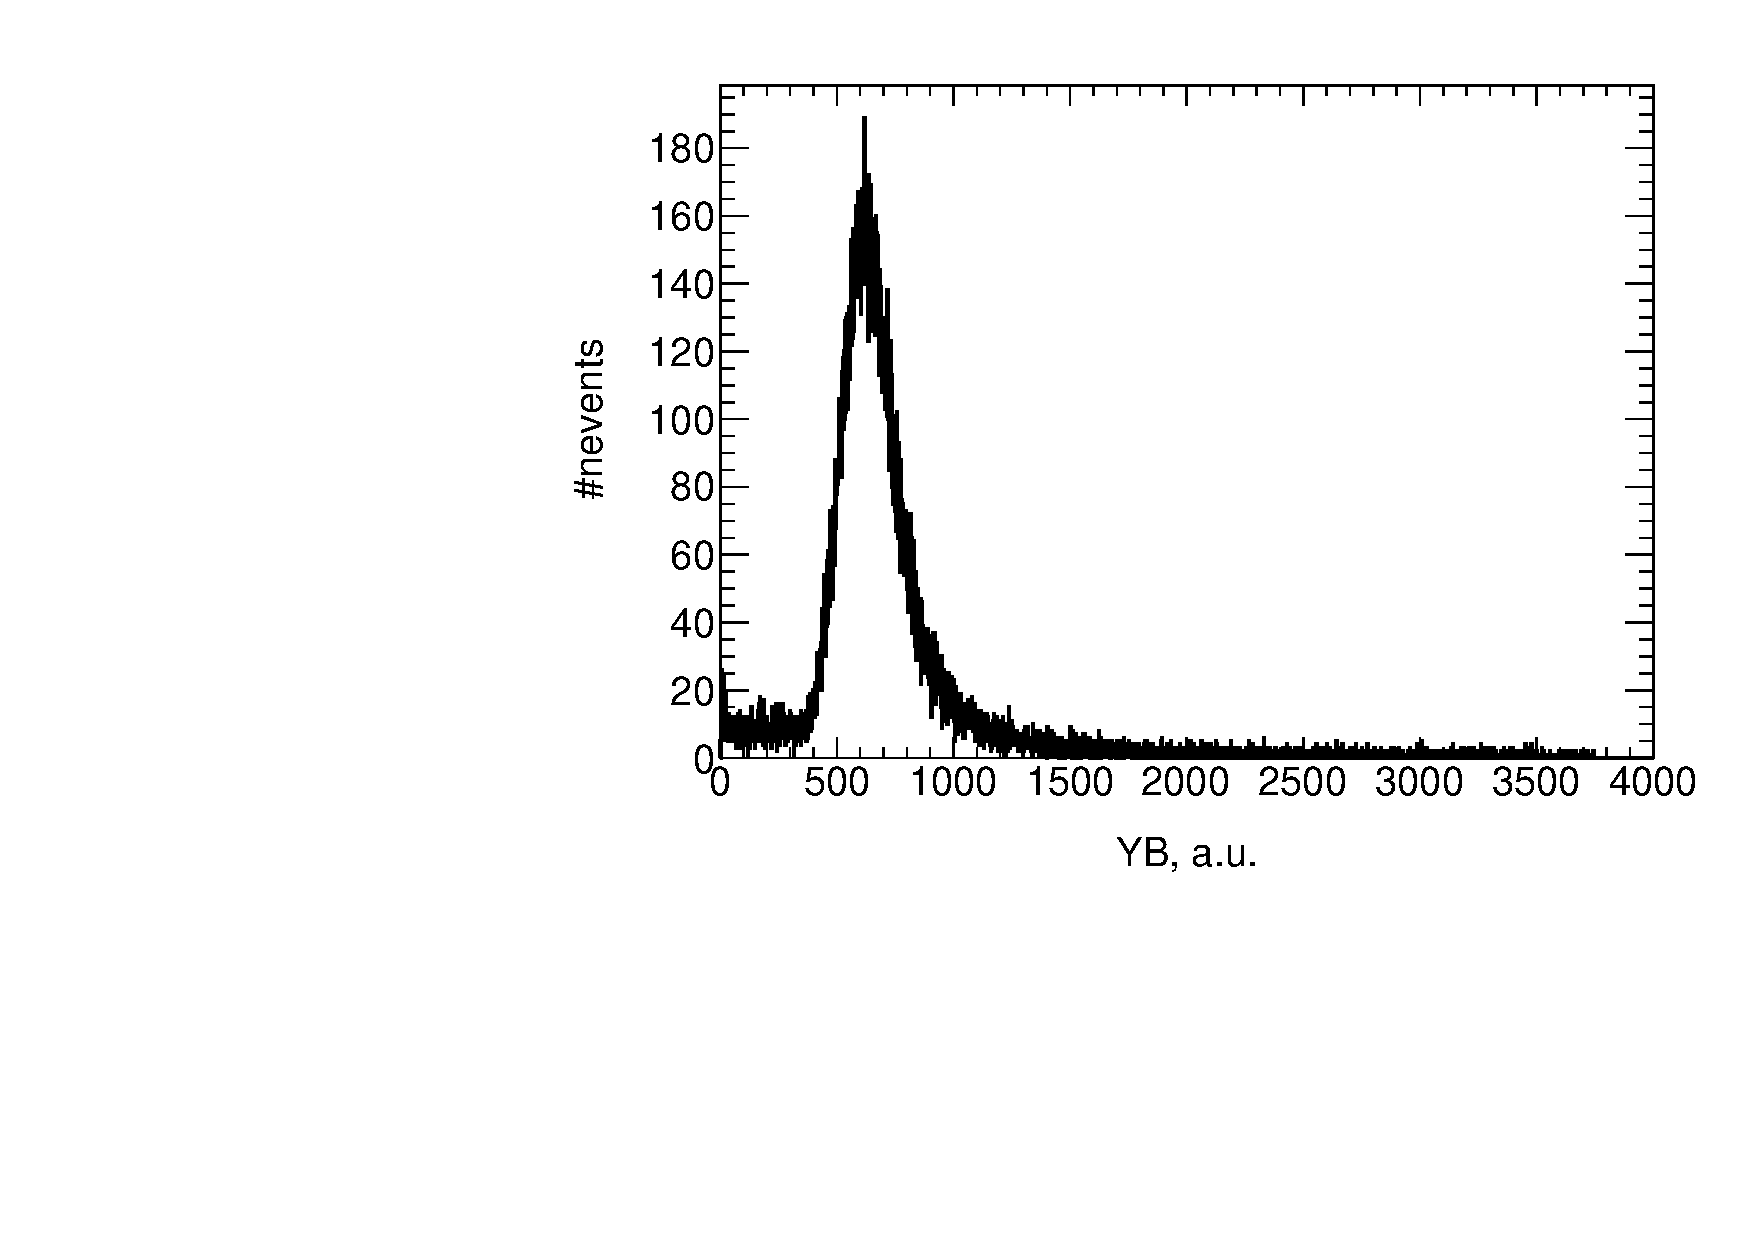
\includegraphics[width=\textwidth]{yb.pdf}
			\caption{}\label{}
		\end{subfigure}
\hspace*{\fill}
	\caption{Weighted signal amplitude distribution on run 1463 (pion beam).}\label{y_signals}
\end{figure}

\begin{figure}[ht]
	\hspace*{\fill}
	\centering
	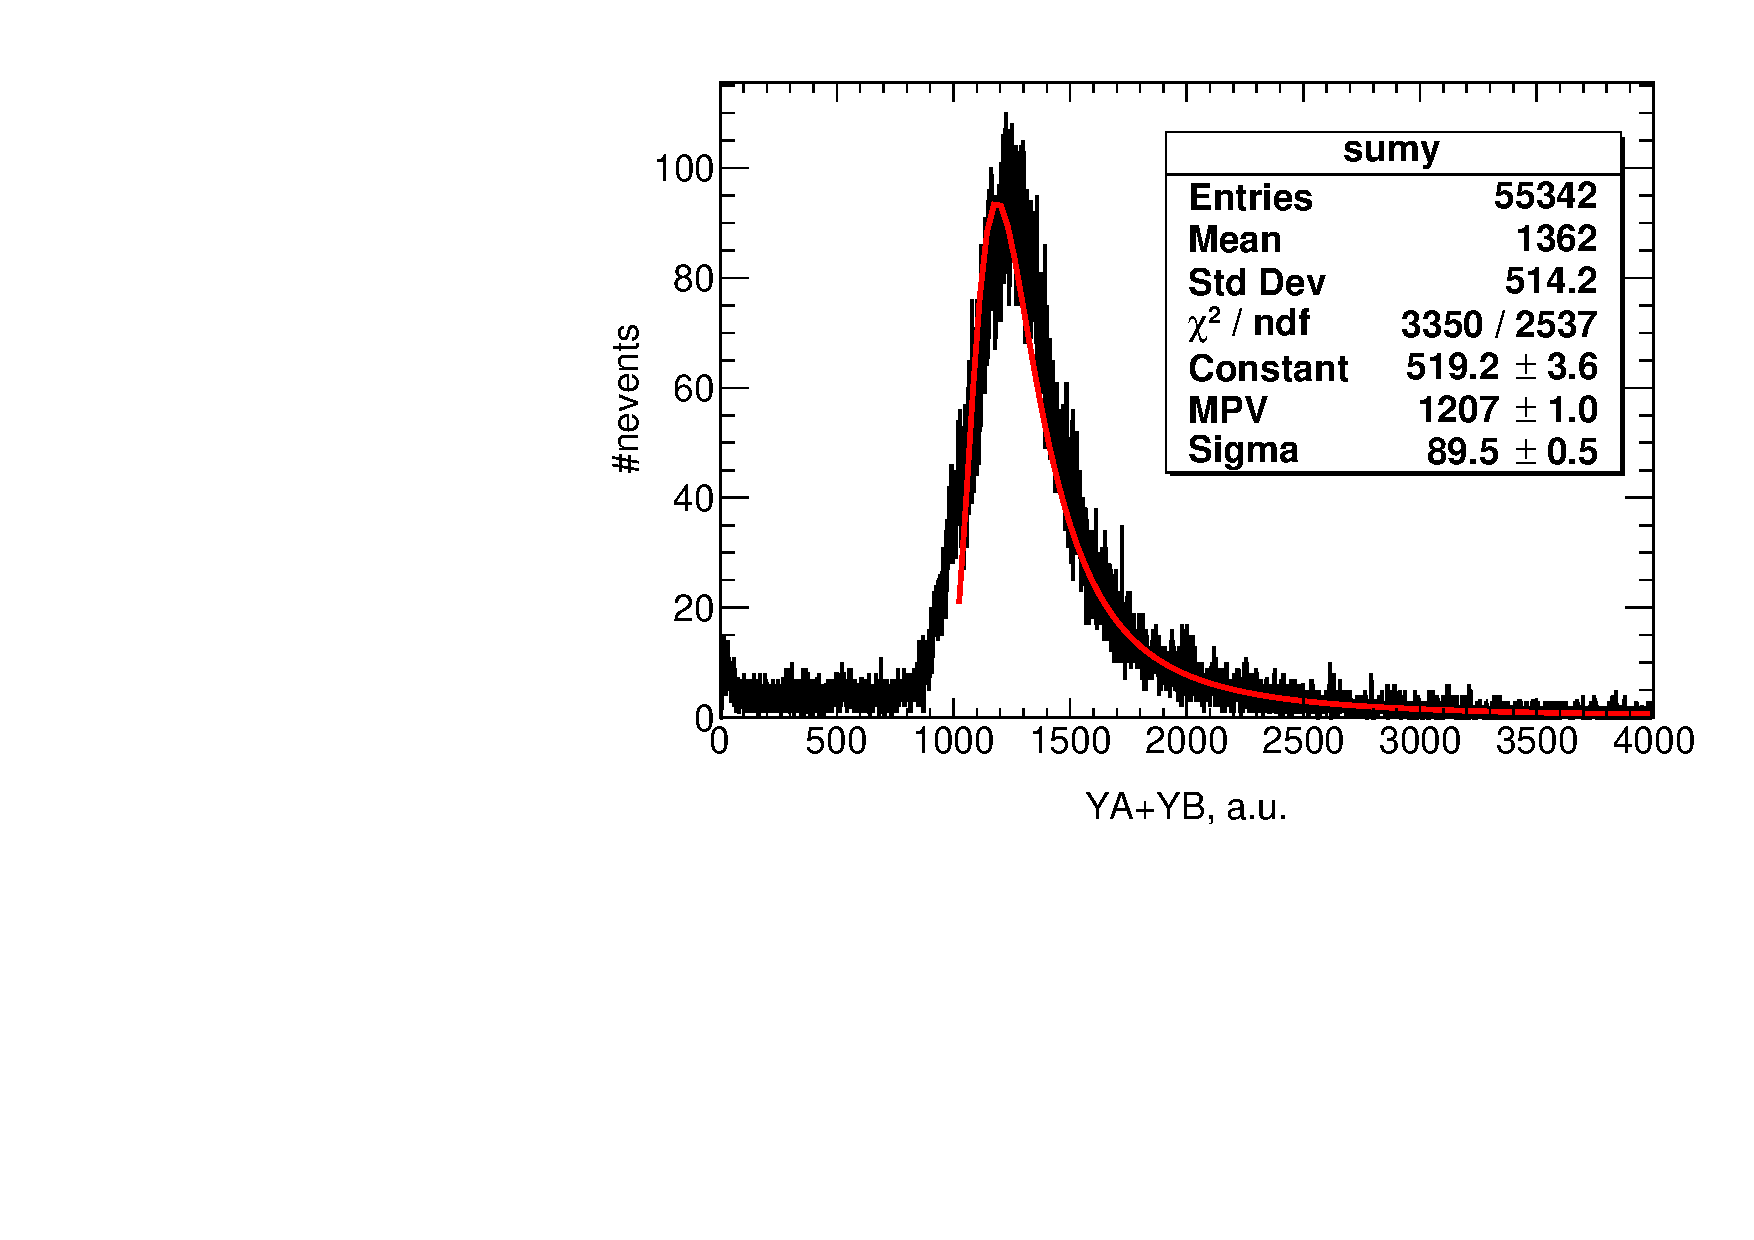
\includegraphics[width=0.6\textwidth]{sumy.pdf}
	\hspace*{\fill}
	\caption{}\label{y_sumab}
\end{figure}

The charge division circuit was made to obtain the position of the particles crossing the detector along y-side. The
position is obtained according to equation \ref{AplusB}. On the other hand, to calculate the position on the x-side, a
different treatment must be done. Using a simple center of mass calculation for each x channel the position can be
estimated like:

\begin{equation}
X_{\mathrm{pos}}=\frac{\sum_{x=0}^{24} E[x]*x}{\sum_{x=0}^{24} E[x]}
\end{equation}
where $x$ represent the channel number and $E[x]$ the energy deposited on that channel. The Figure \ref{position} shows
the position distribution of the beam for each triggered event. About 6 columns of crystals (strips) are fired, while in
y-side 9 strips are fired resulting in a beam size of 2.4x3.6\SI{}{cm^2}.  

\begin{figure}[ht]
	\hspace*{\fill}
	\centering
		\begin{subfigure}[b]{0.45\textwidth}
			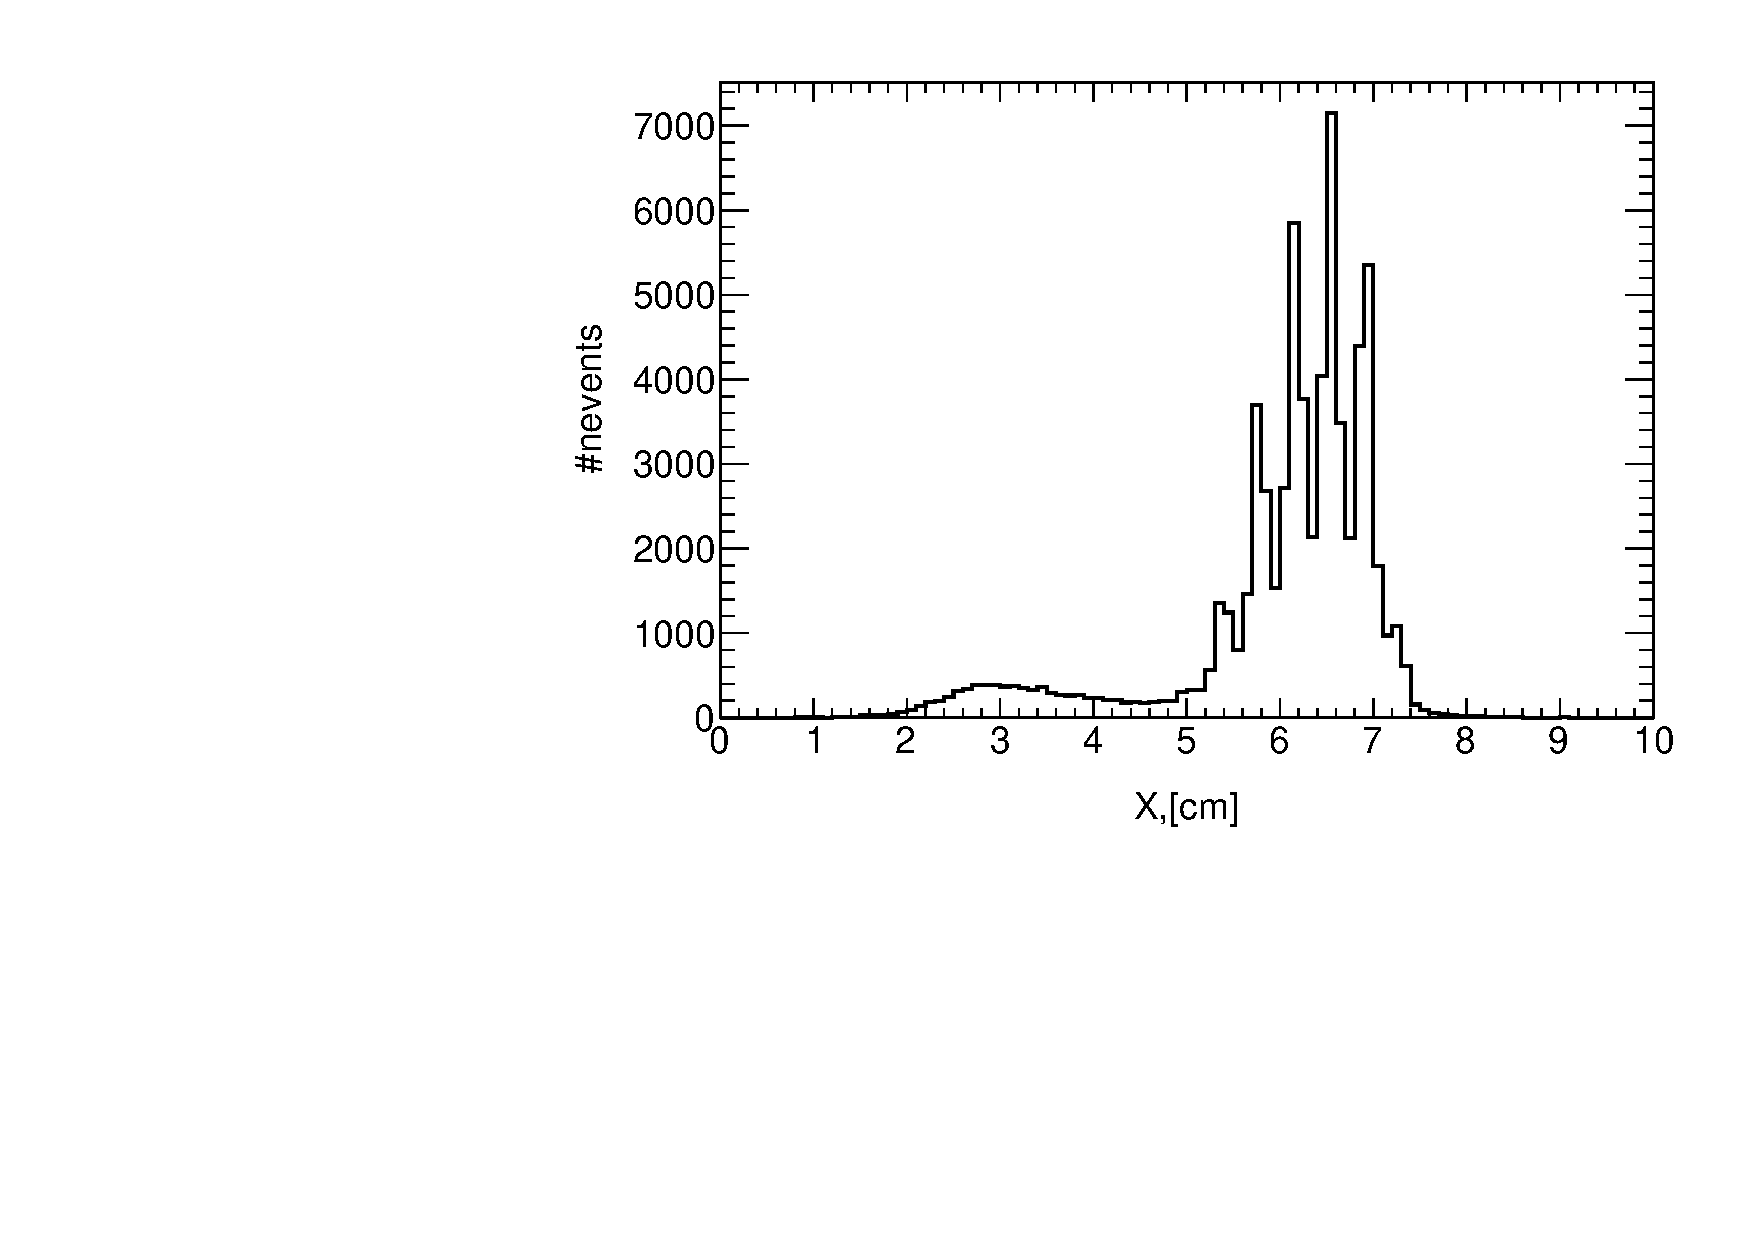
\includegraphics[width=\textwidth]{posx.pdf}
			\caption{X-axis position}\label{xpos}
		\end{subfigure}
		\hfill
		\begin{subfigure}[b]{0.45\textwidth}
			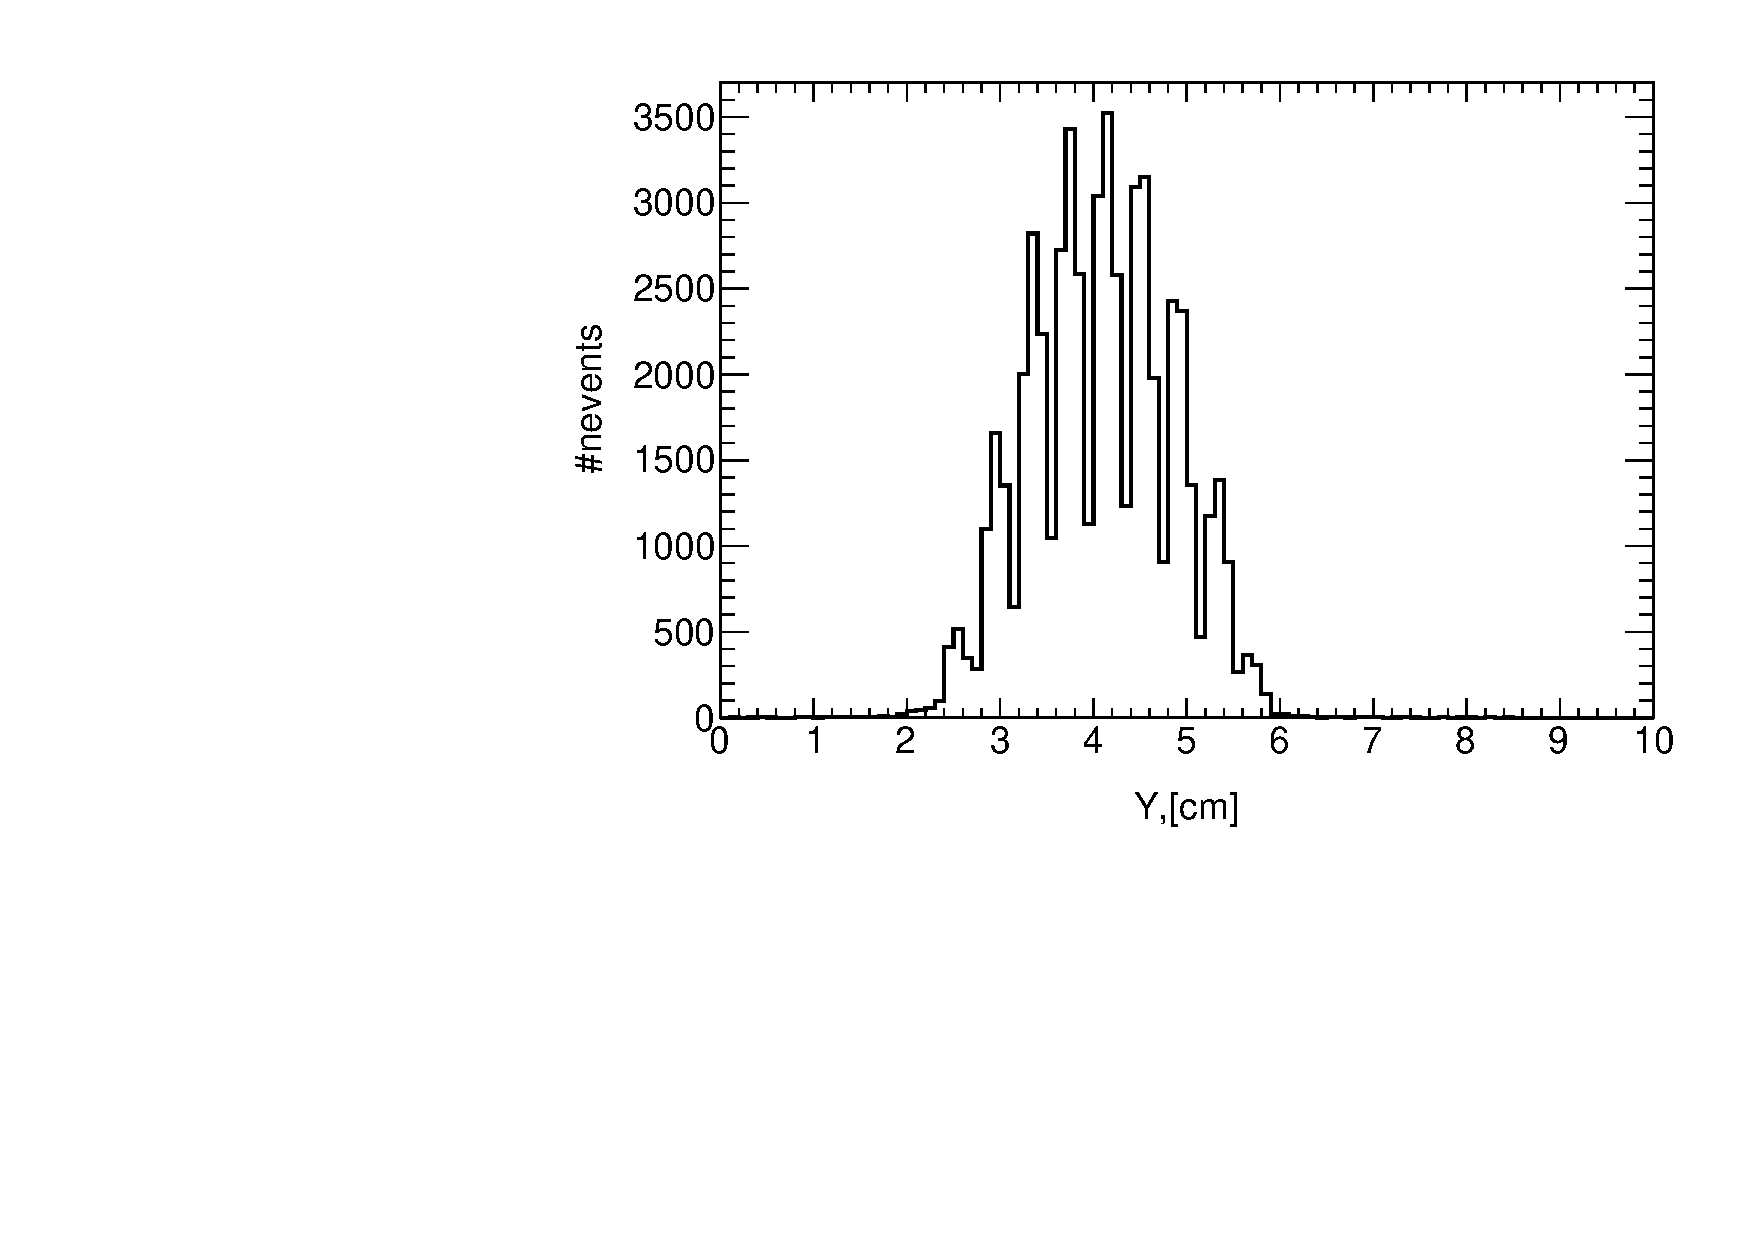
\includegraphics[width=\textwidth]{posy.pdf}
			\caption{Y-axis position}\label{}
		\end{subfigure}
\hspace*{\fill}
	\caption{Position reconstructed by x and y side using center of mass for X-axis and the equation \ref{AplusB} for
	Y-axis.}\label{position}
\end{figure}
To ensure the quality of the equalization two set of runs were taken with pion beam. Where the results for Run 1467 are
present in the previous figure. The Run 1468 differ from the previous one by the beam position. The moving table were
the LYSO detector is placed was moved by 3 centimeters. So it could be possible to figure out what are the small events
present in the x position graph \ref{xpos} presented from centimeter 2 to 5. \par

The gaussian like distribution on the first 5 centimeters remain after move the beam and represent a change in the
pedestal on these channels for this particulars runs.\par
\begin{figure}[ht]
	\hspace*{\fill}
	\centering
		\begin{subfigure}[b]{0.45\textwidth}
			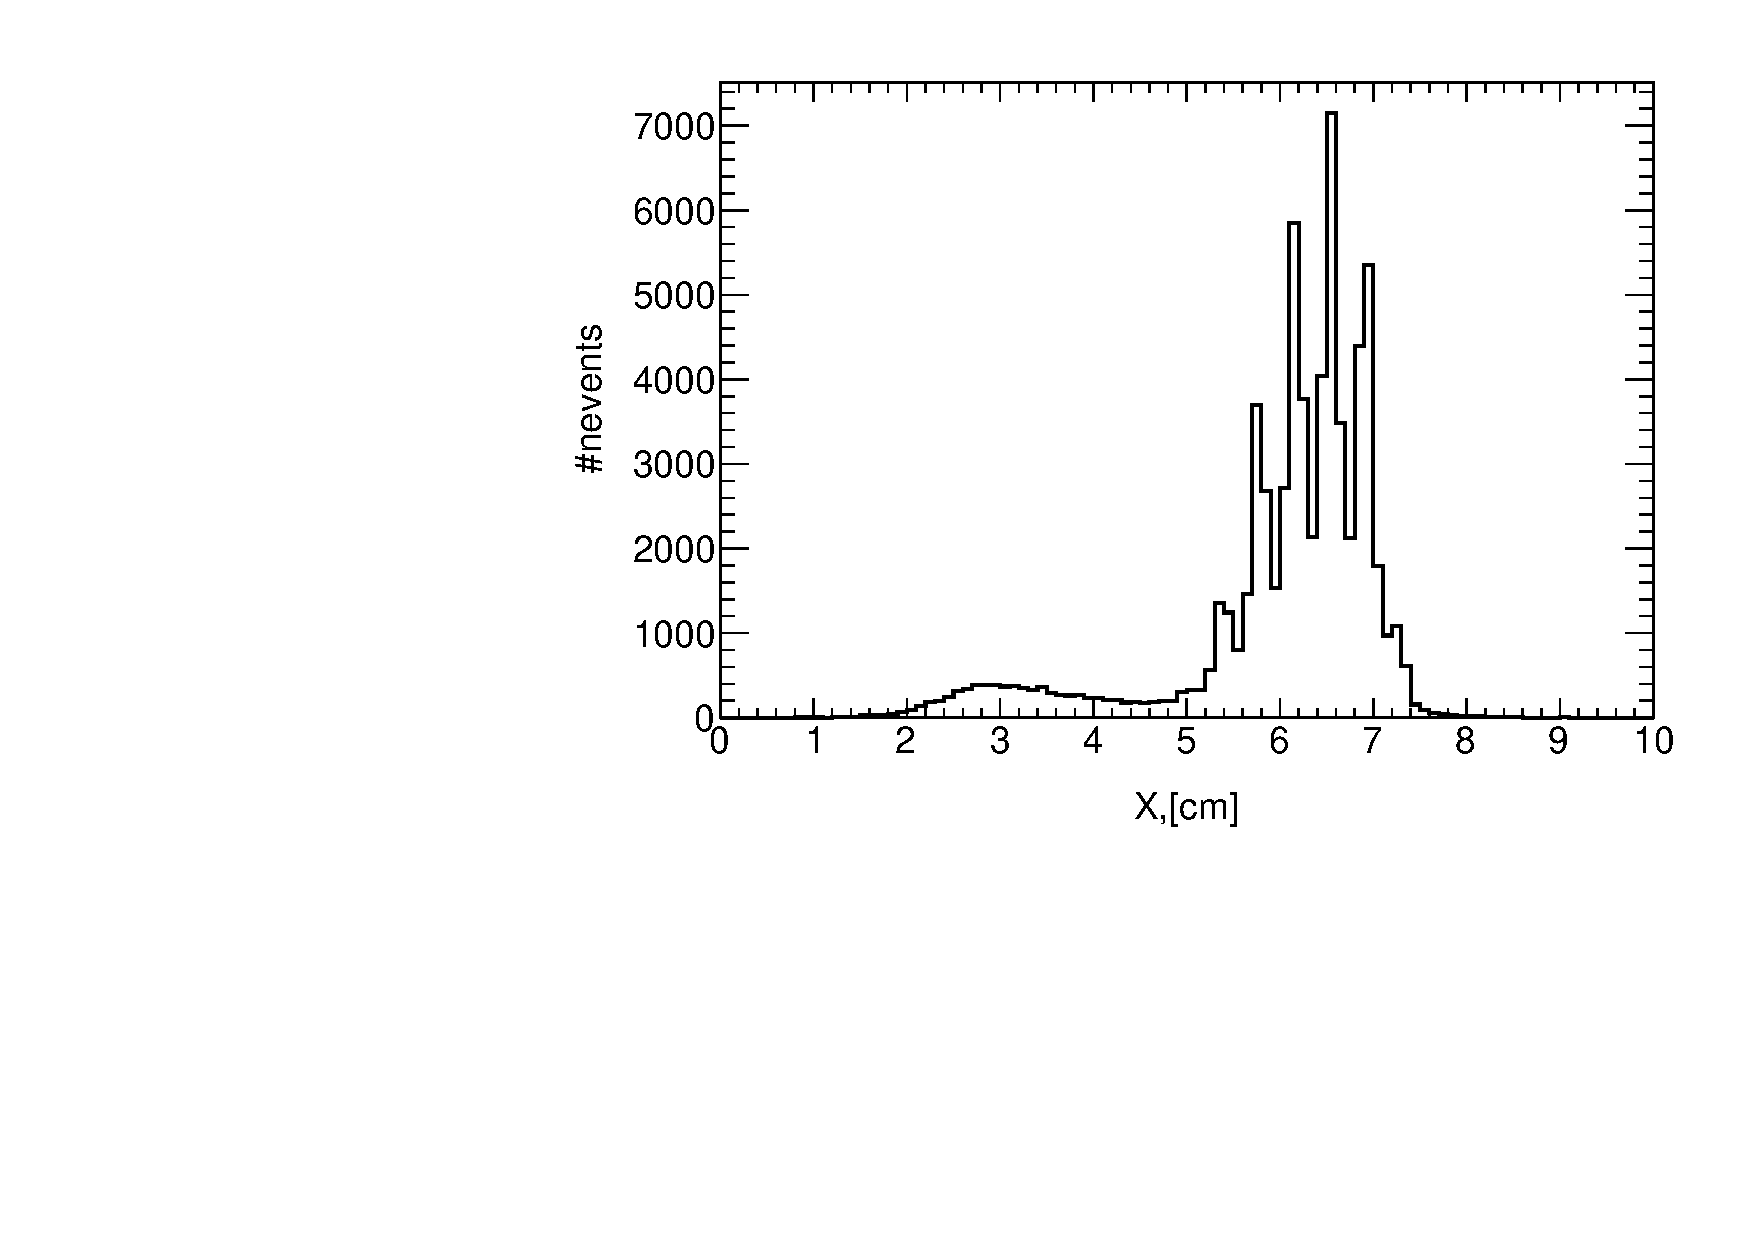
\includegraphics[width=\textwidth]{posx.pdf}
			\caption{run 1467}\label{xpos}
		\end{subfigure}
		\hfill
		\begin{subfigure}[b]{0.45\textwidth}
			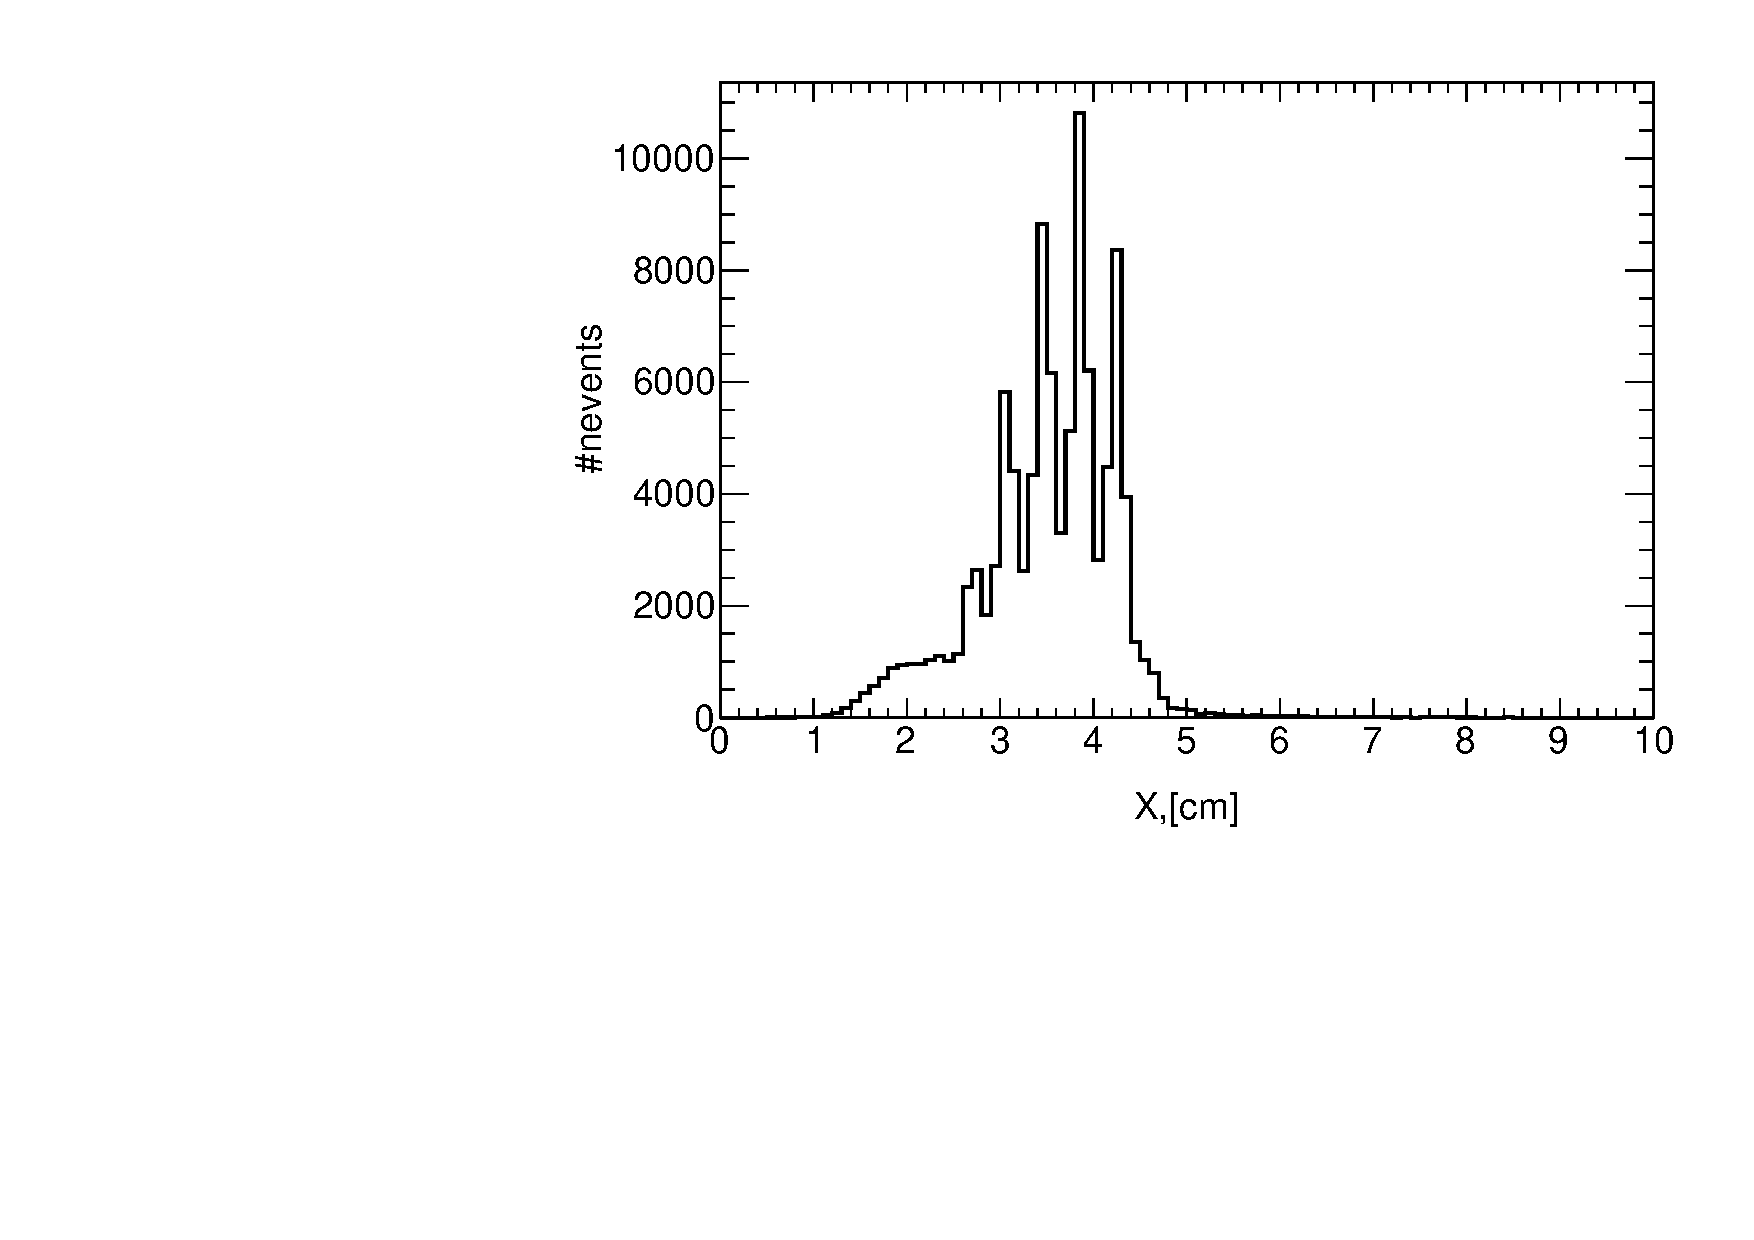
\includegraphics[width=\textwidth]{posx1468.pdf}
			\caption{run 1468}\label{}
		\end{subfigure}
\hspace*{\fill}
	\caption{X position comparrison from Run 1467 y 1468.}\label{position}
\end{figure}

Using both distribution, x and y position is possible to obtain a 2D profile of the pion beam on the detector. This
profile highlight the crystal matrix present in the detector. 

\begin{figure}[ht]
	\hspace*{\fill}
	\centering
		\begin{subfigure}[b]{0.45\textwidth}
			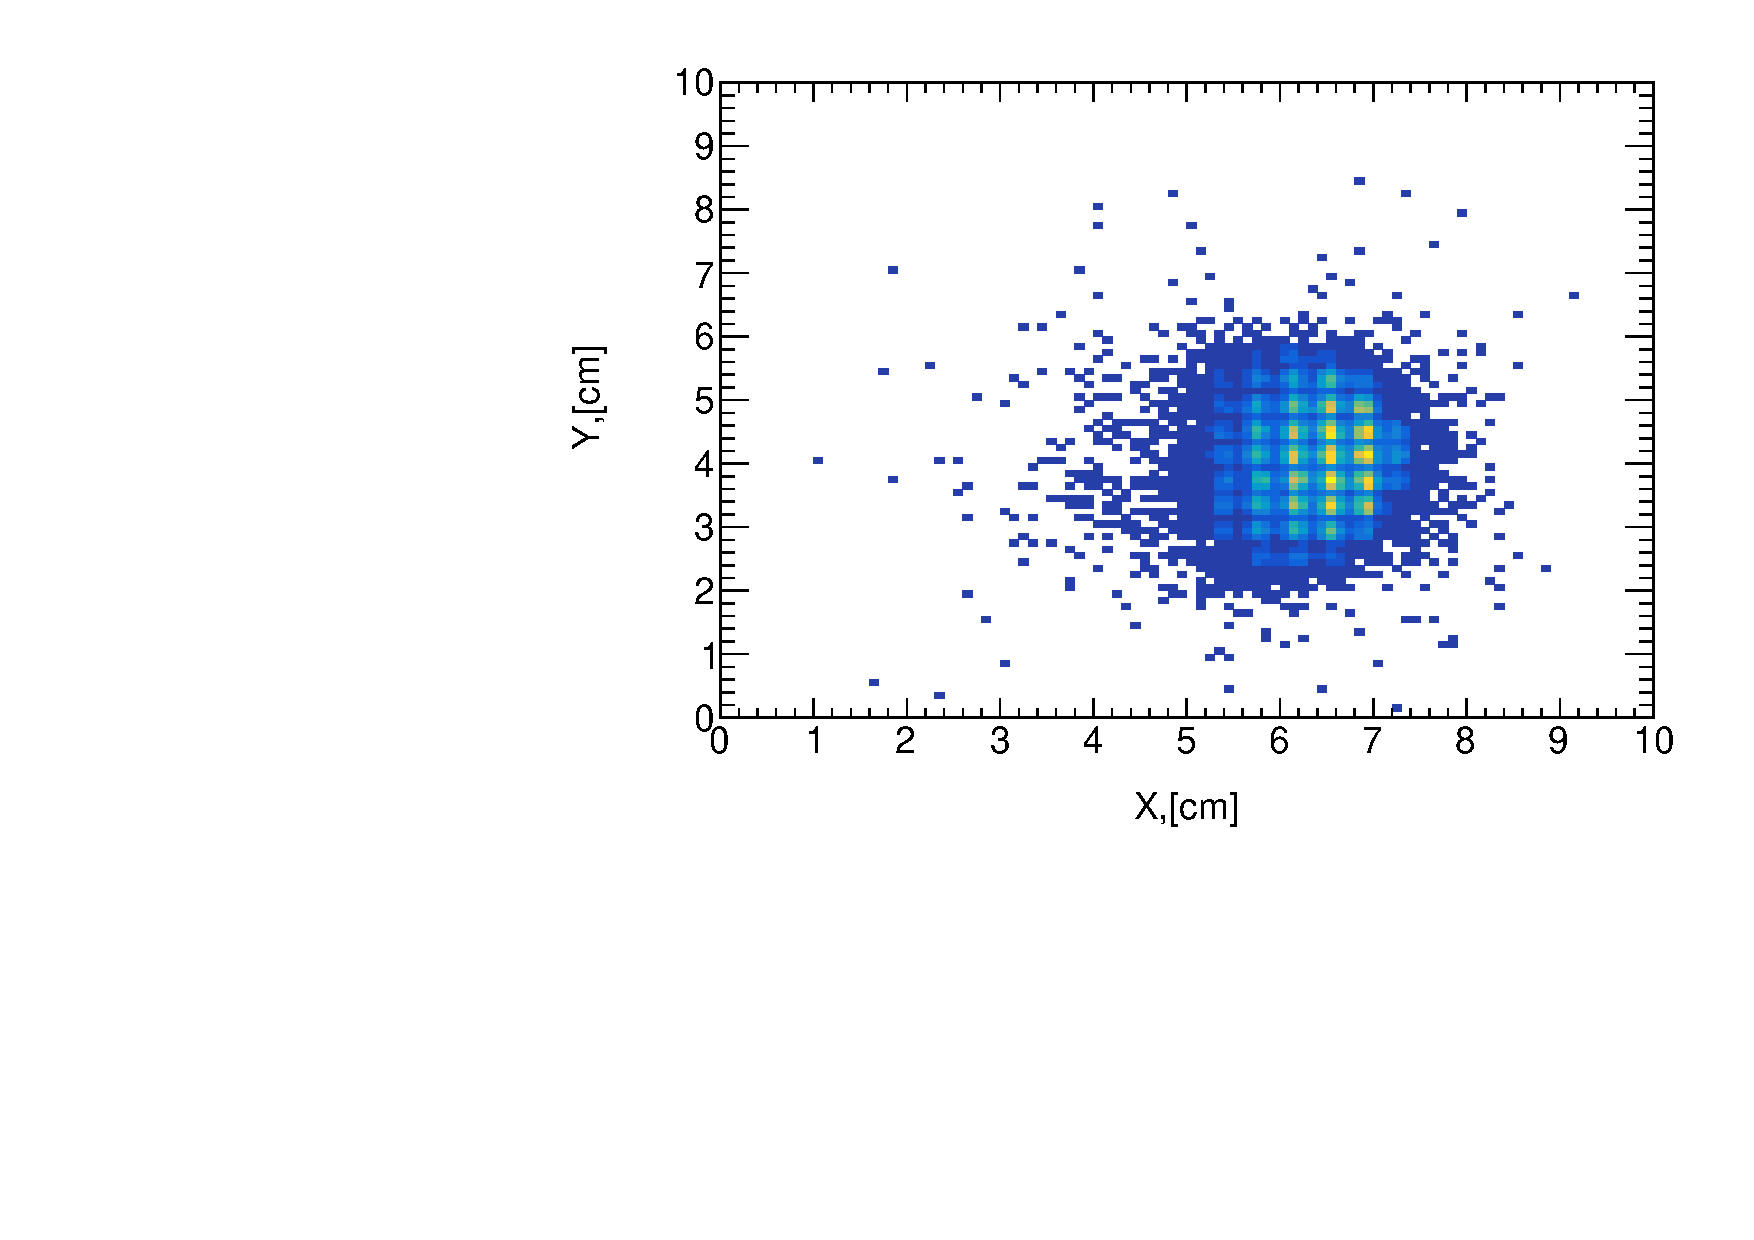
\includegraphics[width=\textwidth]{profile1467.pdf}
			\caption{Run 1467}\label{}
		\end{subfigure}
		\hfill
		\begin{subfigure}[b]{0.45\textwidth}
			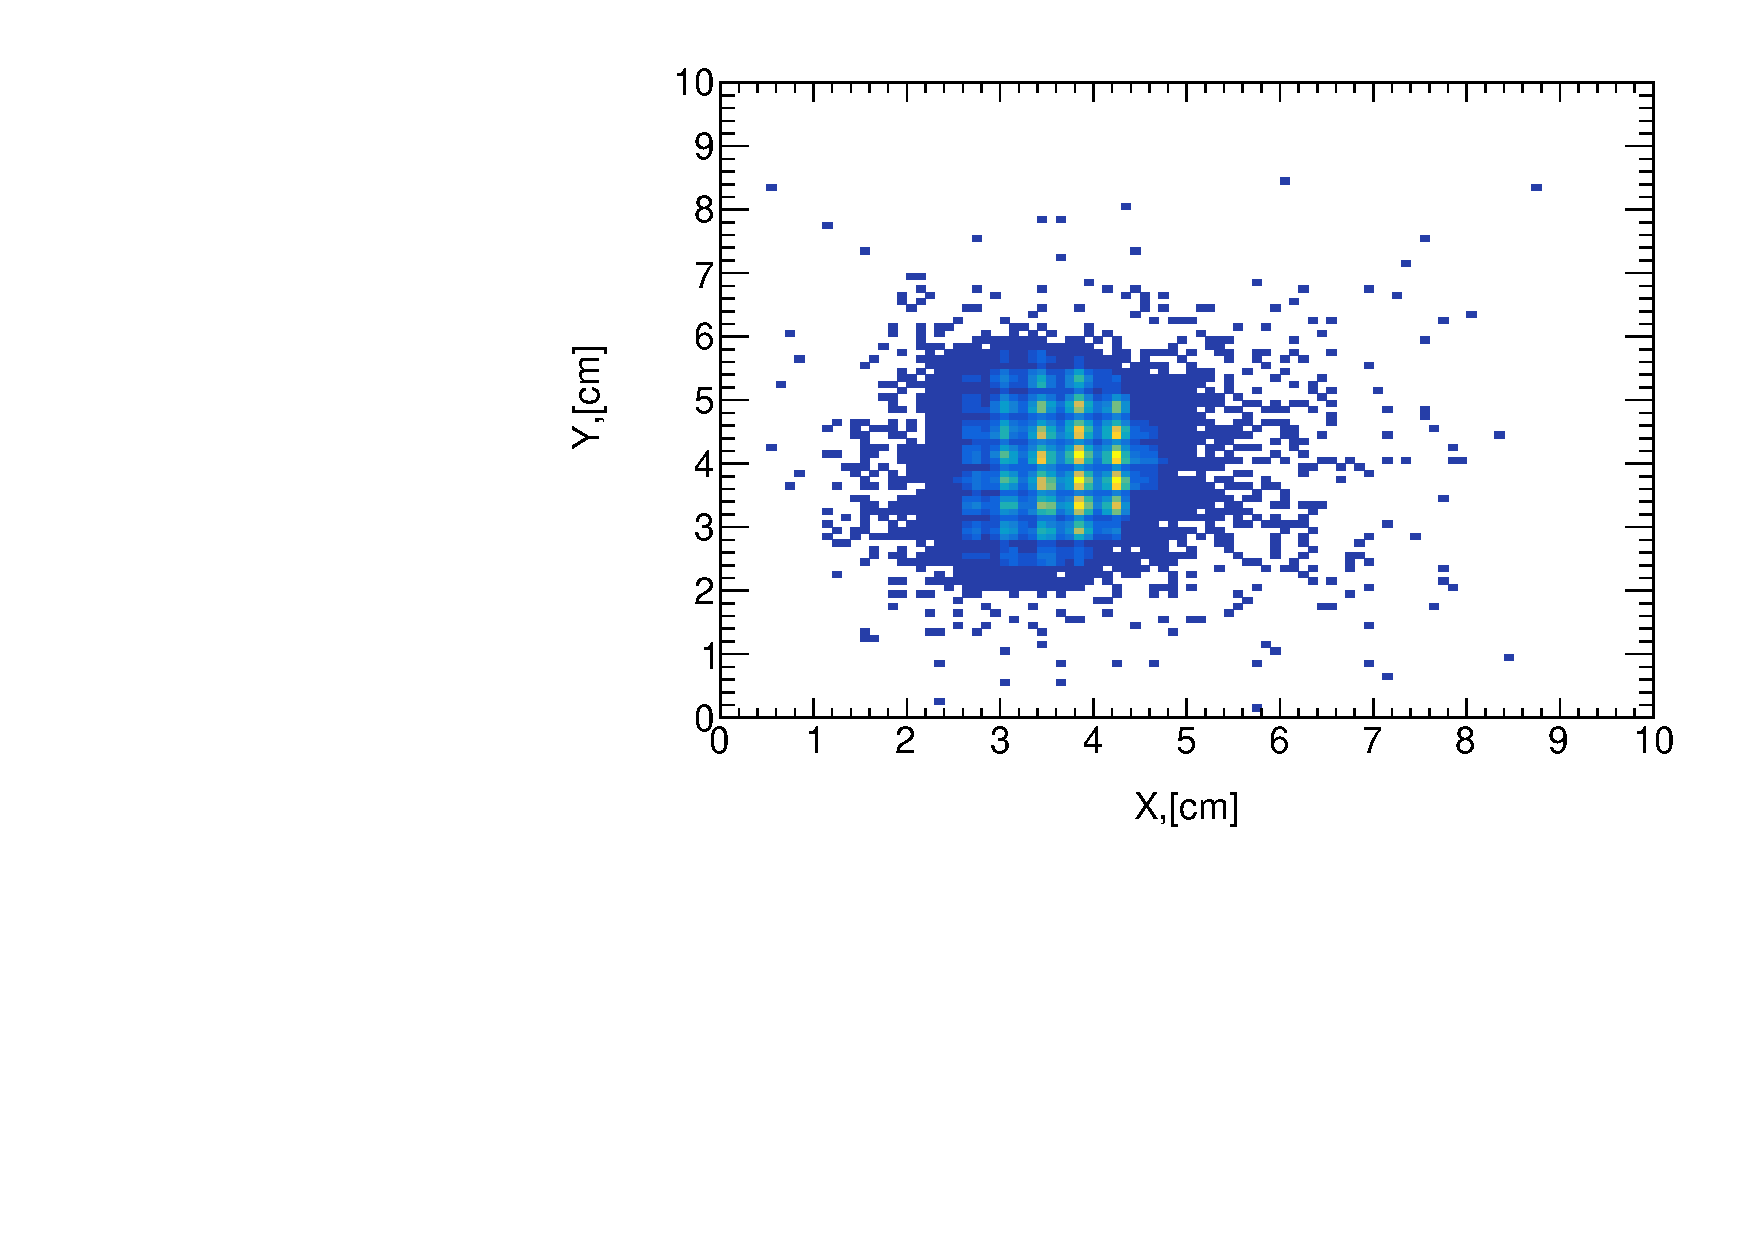
\includegraphics[width=\textwidth]{profile1468.pdf}
			\caption{Run 1468}\label{}
		\end{subfigure}
\hspace*{\fill}
	\caption{Beam profile for two diferent pion runs, with with different x position.}\label{profile}
\end{figure}






\section{Time resolution}
\begin{figure}[ht]
	\hspace*{\fill}
	\centering
	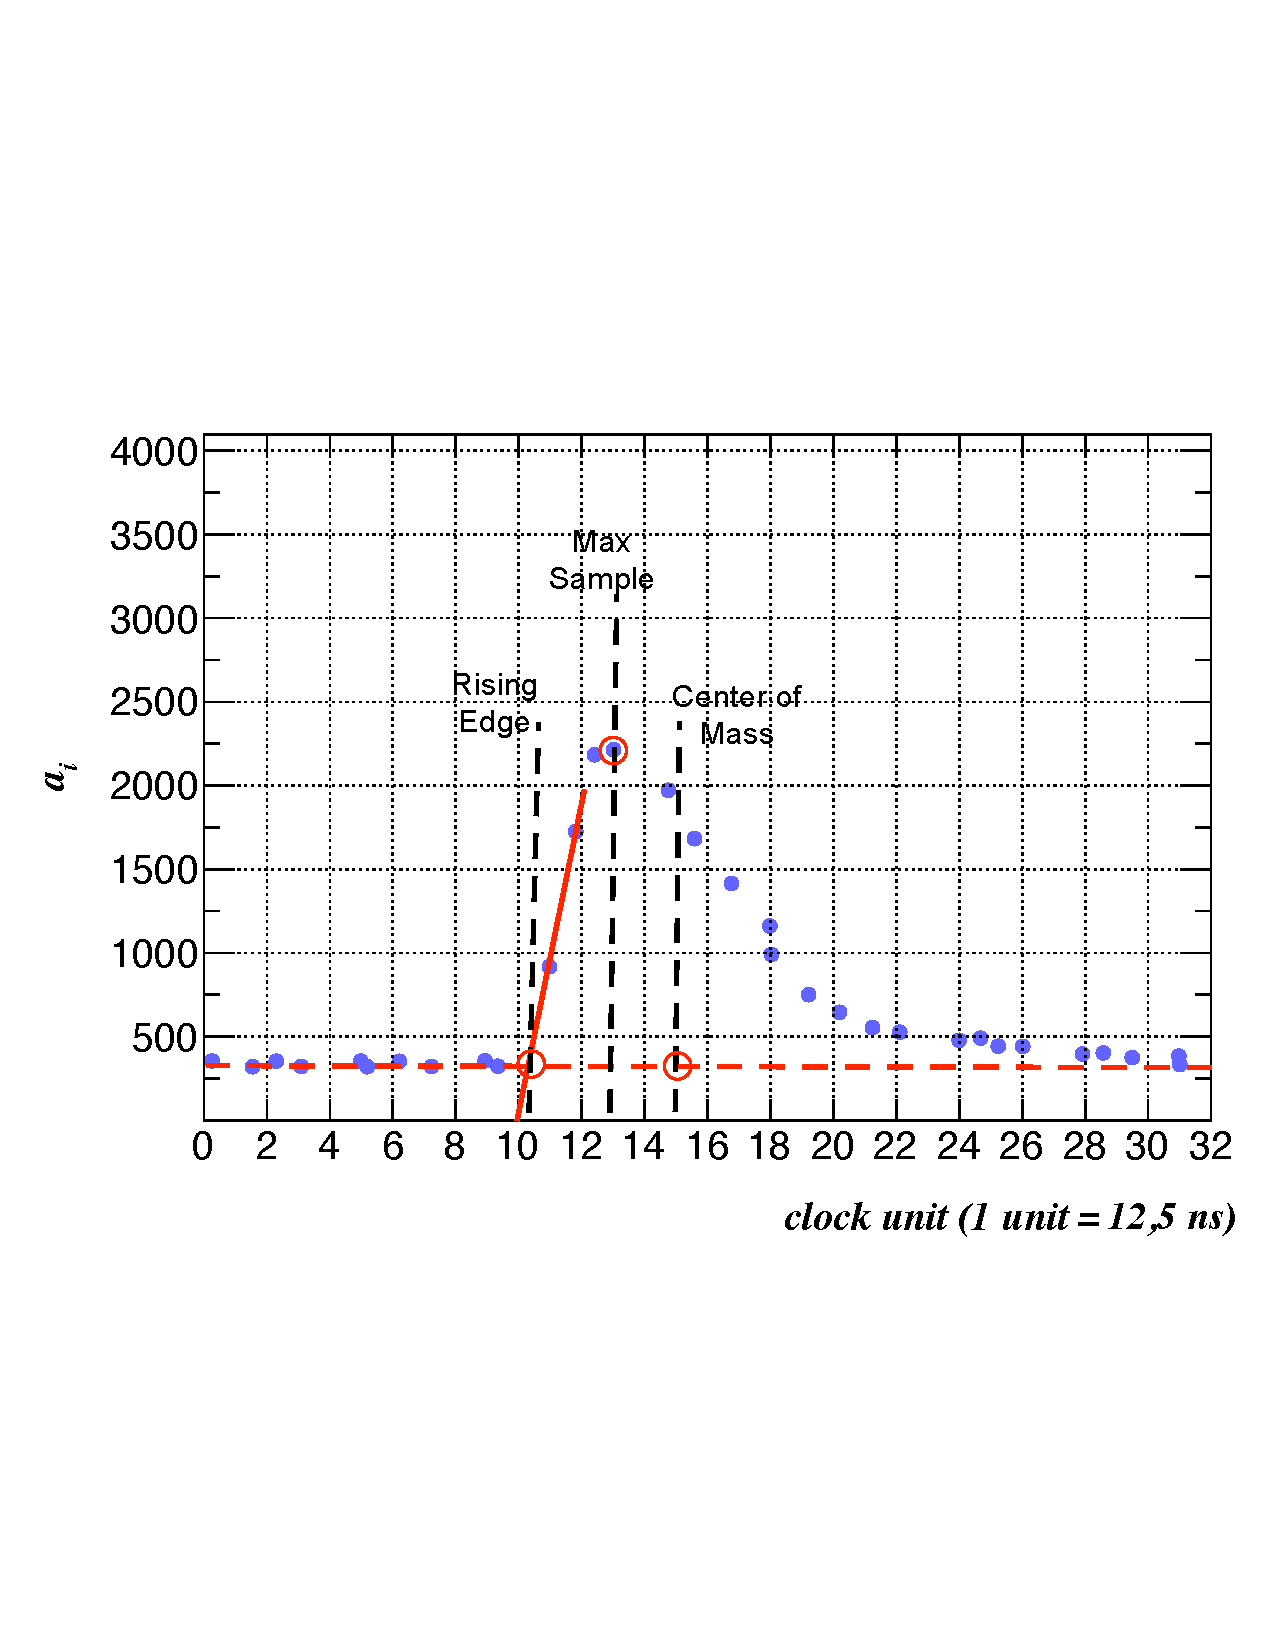
\includegraphics[width=0.6\textwidth]{t0_sample.pdf}
	\hspace*{\fill}
	\caption{Timing methods on wave sample}\label{}
\end{figure}

In order to estimate the timing for each detector, the time reference is the first counter upstream. According to the
setup show in Figure \ref{fig:na64detector}, the first counter is the scintillator $S1$. \par
To calculate the timing from the 32 time samples, three methods were applied.\par


\begin{figure}[hb]
	\hspace*{\fill}
	\begin{subfigure}[b]{0.3\textwidth}
	\centering
	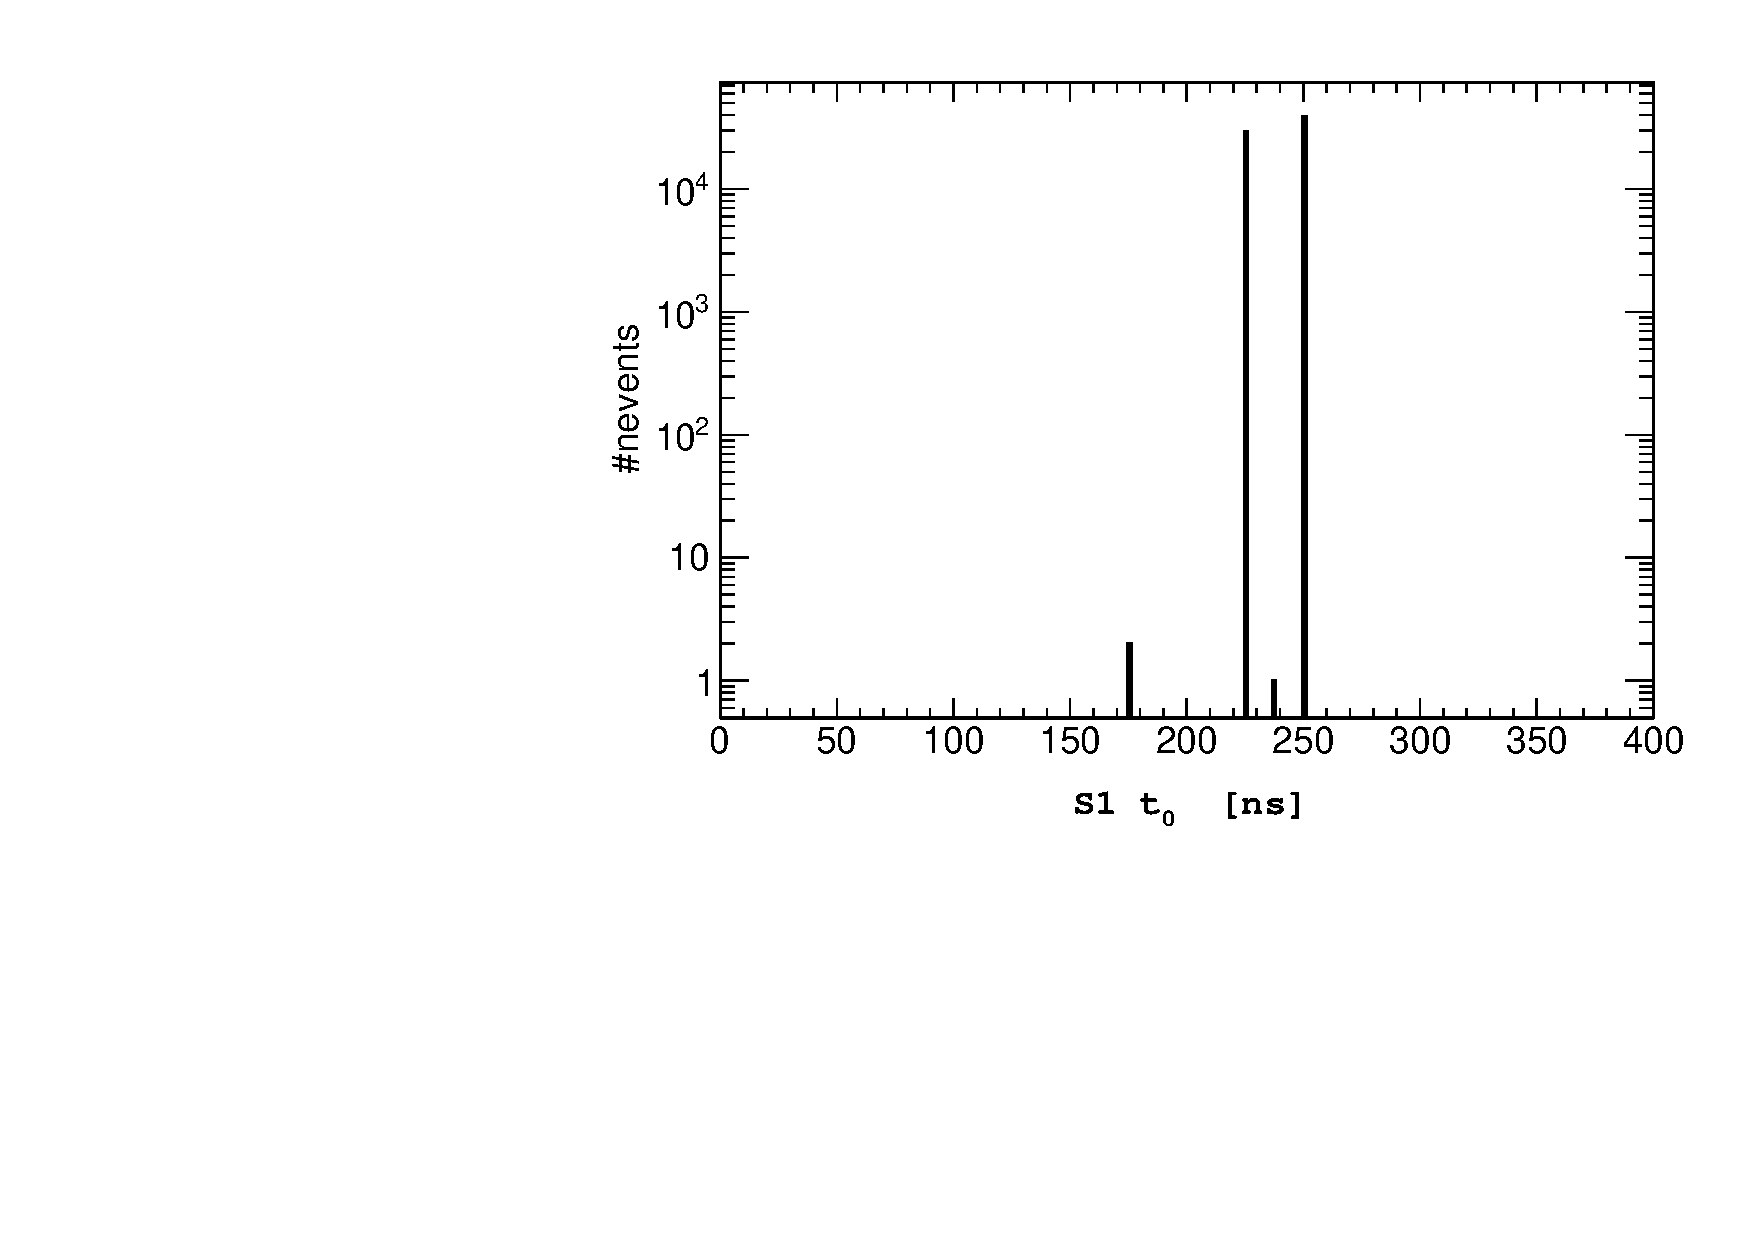
\includegraphics[width=\textwidth]{s1Max.pdf}
	\caption{Max Sample}\label{}
	\end{subfigure}
	\begin{subfigure}[b]{0.3\textwidth}
	\centering
	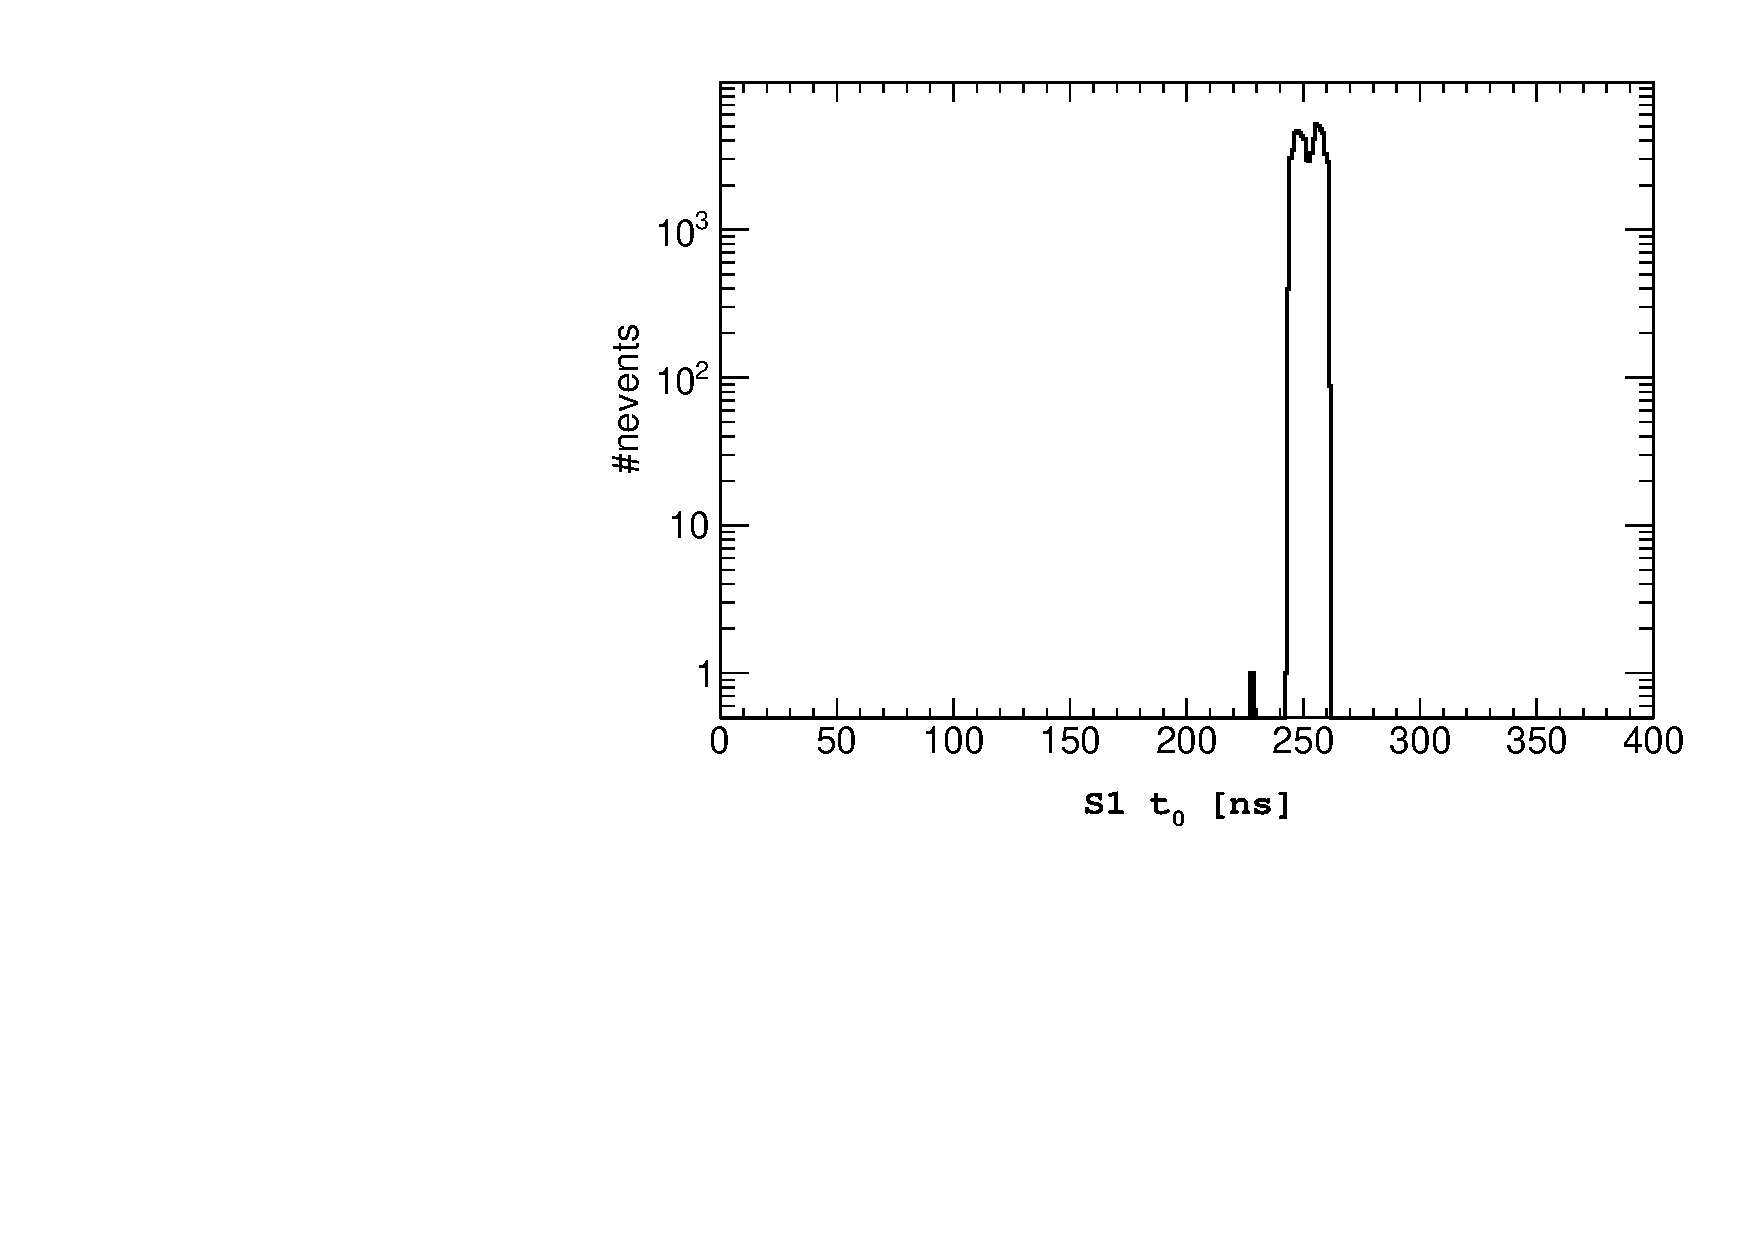
\includegraphics[width=\textwidth]{s1CoM.pdf}
	\caption{Center of Mass}\label{}
	\end{subfigure}
	\begin{subfigure}[b]{0.3\textwidth}
	\centering
	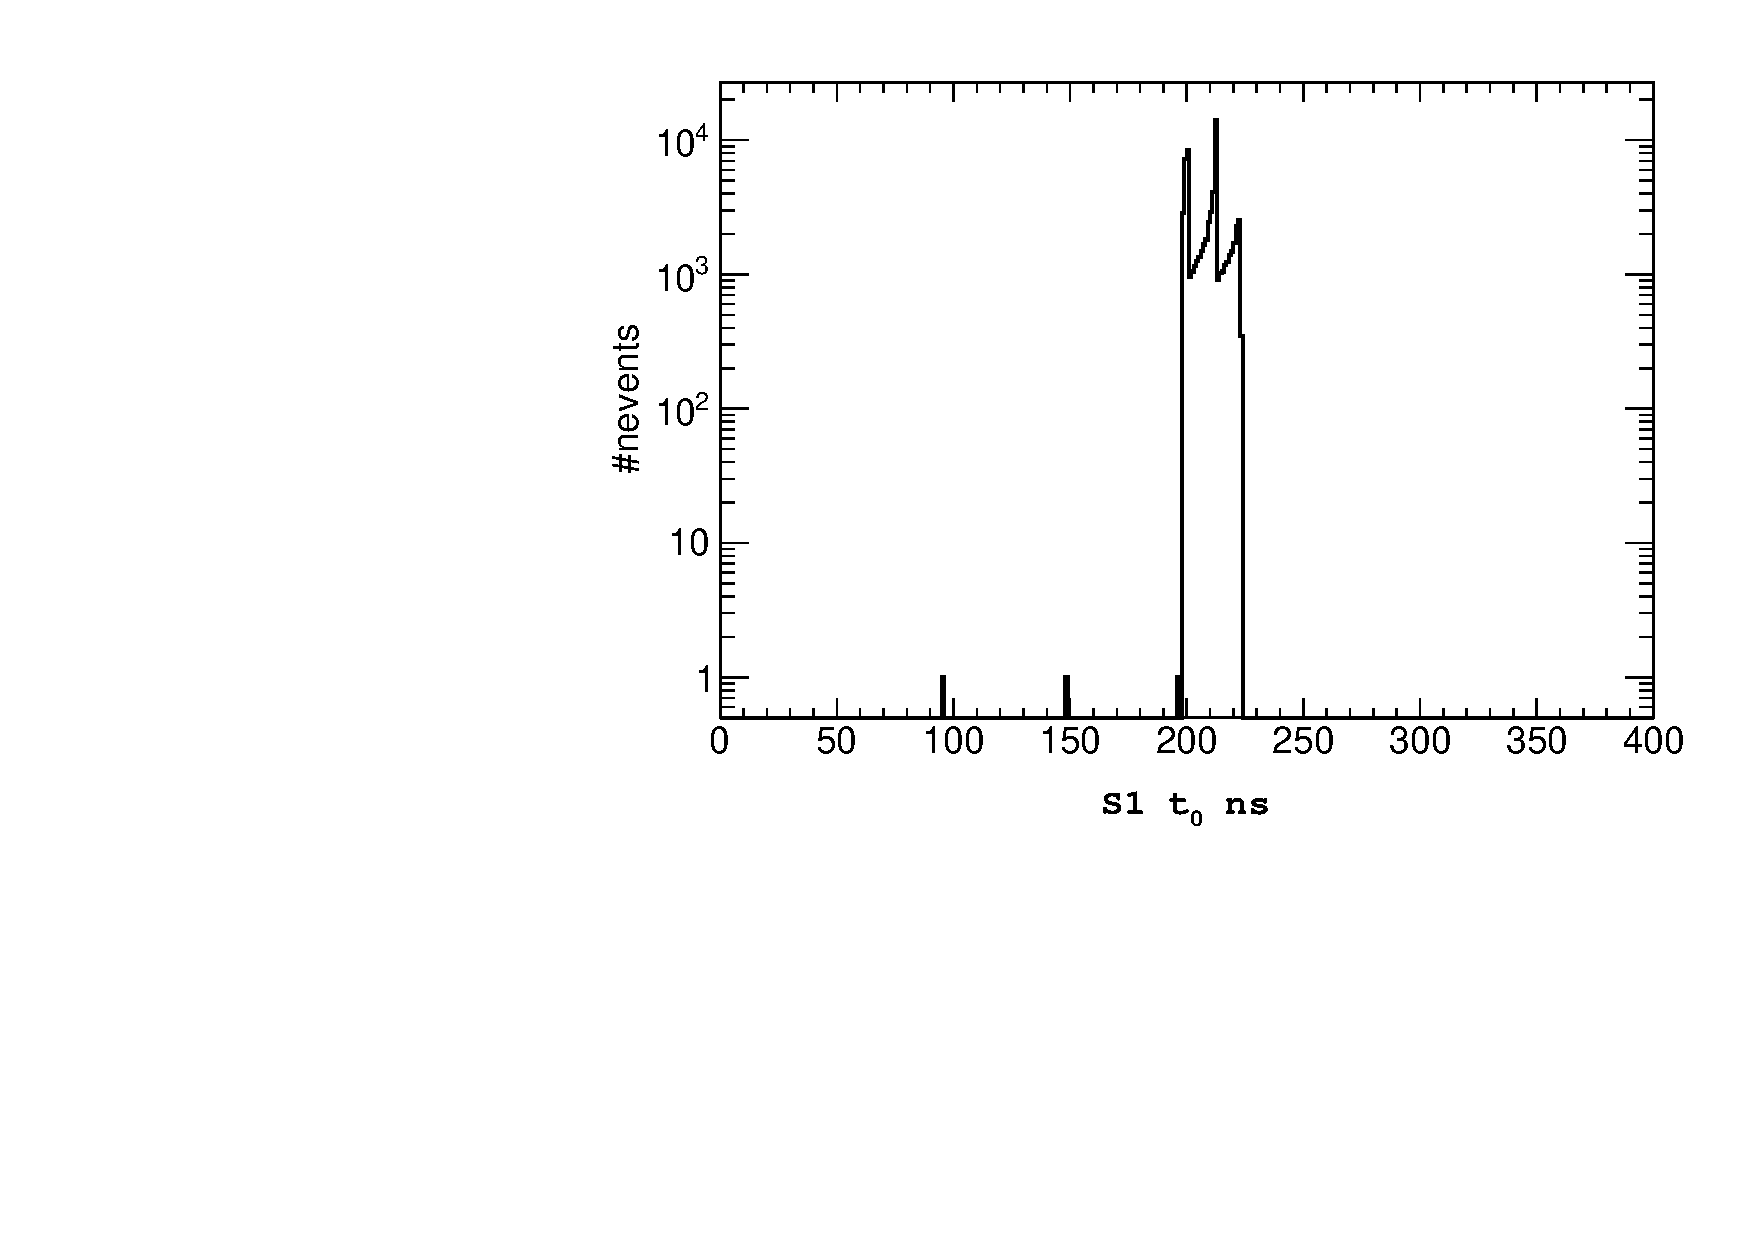
\includegraphics[width=\textwidth]{s1RE.pdf}
	\caption{Rising Edge}\label{}
	\end{subfigure}\hspace*{\fill}
	\caption{Timing calculated for S1 with three diferent methods; Max sample, Center of Mass and Rising Edge. }\label{}
\end{figure}



\subsubsection{Max sample}

From the 32 time samples, the max amplitud is recorded and the time sample when this happend is set as the time $t_0$.
This method is very sensity to saturation of the ADC range. The scintillitor counters reach easyle the maximum ADC
counts, and then timing will be independent of the max amplitud reached by the detector.\par
The Figure \ref{t0m} shows the $t_0$ distribution calculated with this method. The majority of the events the counter
$S1$ saturate the ADC, therefore, two sharp peaks are present at 237ns(12,5*19) and 250ns(12,5*20). Separated exactly
12,5 ns  shows that the counter is saturated at the same time sample, either in one ADC or in the next one.\par


\subsubsection{Center of Mass}
This method estimate the center of mass of each pulse, and the result represent $t_0$. The center of mass for one pulse
is calculated as :

\begin{equation}
t_0= \frac{\sum_{i=8}^{31}a_i*i}{\sum a_i}
\end{equation}

which consider the amplitudes $a_i$ after the time samples for pedestal estimation. Only the time samples after 8 are
considered. 

\subsubsection{Rising Edge}

The last method calculate the intersection of the rising edge with the time axis to get the origin time ($t_0$).
Again using the maximum of amplitud, the algorithym look for the time sample with half of the maximum or above and
return the index of the time sample. Aftewards, from the time sample with half of the maximum ($a_{j}$) and the
previous one $a_{j-1}$ is possible to obtain the intersection of this linear with the axis time.\par



\begin{equation}
t_0 = t_j - \frac{a_j}{a_j-a_{j-1}}
\end{equation}
This method present the advantage of being non-sensitive to saturation, because of the use of two time samples before
the saturation occurs and in the worst case when there is no time sample between the base line and the saturated maximum
the origin time will be the time sample before the saturation. \par


Time is defined respect to the first counter S1, and calculated with constant fraction method where:....\\
The temporal resolution on a single channel is shown in ..\\
\begin{figure}[ht]
	\hspace*{\fill}
	\centering
	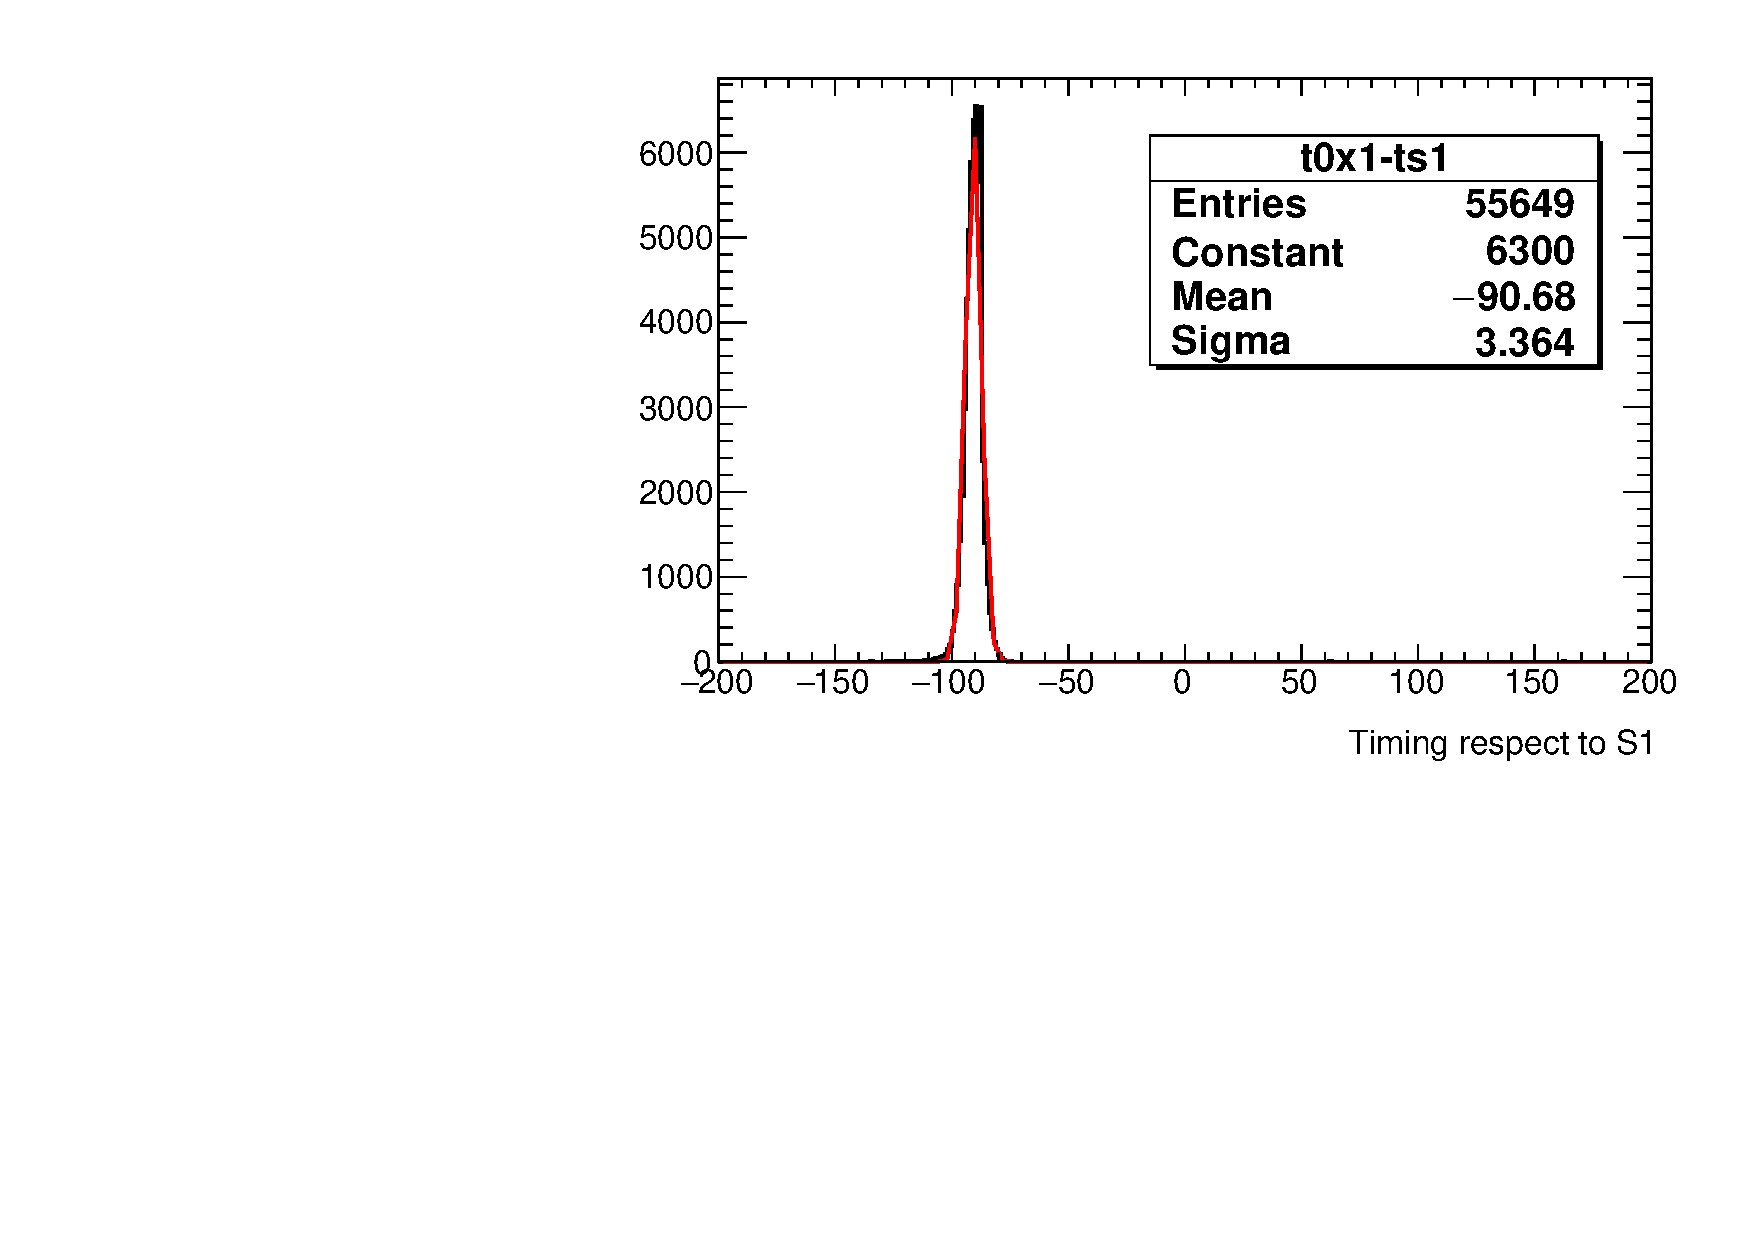
\includegraphics[width=0.5\textwidth]{ts0ts1.pdf}
	\hspace*{\fill}
	\caption{}\label{}
\end{figure}


\section{Hadron rejection}

During the July Run for the NA64 experiment, a set of runs with the LYSO detector as SRD were taken. With an average
beam intensity of 7.5$\cdot 10^5$ events/s registered on S0, these runs are considered low intensity. For tagging the
electrons and reject the hadrons, it is important to know their signature on LYSO. For this purpose, we can exploit two
features of the array of crystals.\par

Each signal from the x-axis, correspond to the amount of light produce by the column of crystals in certain x position.
All the SR produced by the electron beam in the region of the LYSO detector is collected by 25 columns. Therefore, we
should expect a homogeneous distribution of light in these 25 channels. To calculate the amount of hadrons present in
each spill or in the total triggered events, we use the electron (ECAL) and hadron (HCAL) calorimeters to provide the
identification for our analysis.\par


\subsection{BGO hadron suppression}

The crystal were calibrated by comparing the peak position from the energy deposited by minimum ionizing particles with
the one from Monte Carlo simulation, which corresponds about 64MeV. 

\begin{figure}[ht]
	\centering
	\hspace*{\fill}
	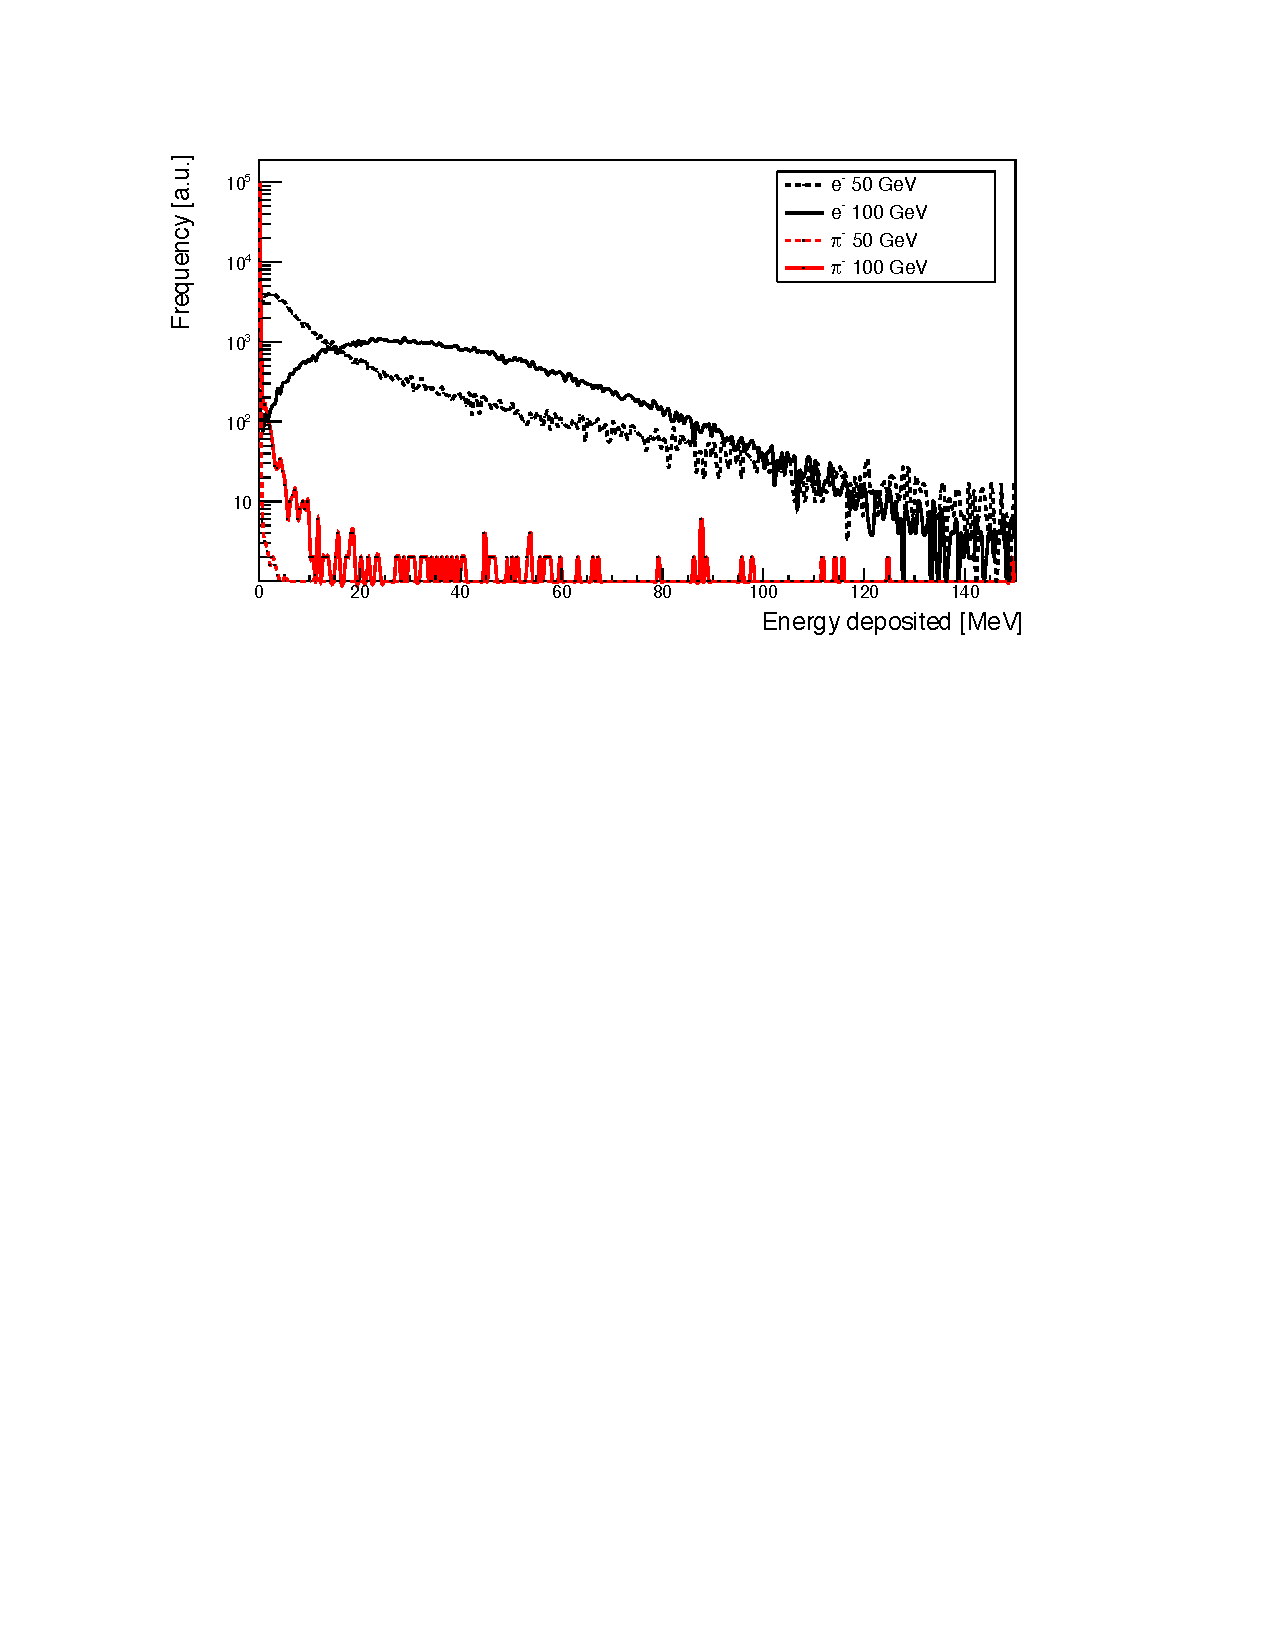
\includegraphics[width=0.8\textwidth]{bgoenergy.pdf}
	\hspace*{\fill}
	\captionsetup{margin=1cm}
	\caption{Results of the GEANT4 simulation for the energy detected by BGO for 50/100 GeV $e^-4$ (black dashed/solid
	line) and 50/100 GeV $\pi^-$ (red dashed/solid line).}\label{bgoe}
\end{figure}


\begin{figure}[ht]
		\centering
		\hspace*{\fill}
		\begin{subfigure}[b]{0.45\textwidth}
			\centering
			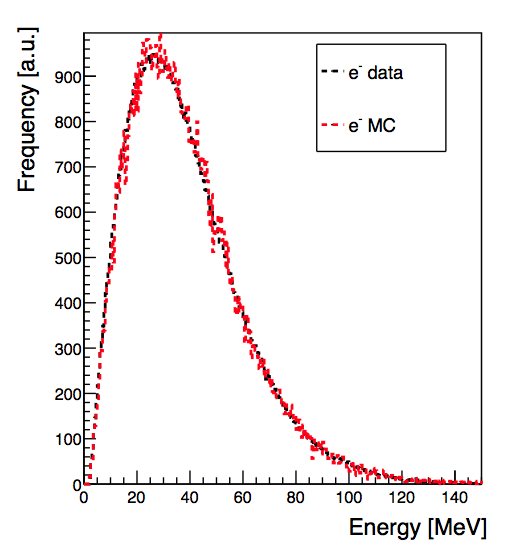
\includegraphics[width=\textwidth]{bgoe.png}
			\caption{}\label{}
		\end{subfigure}
		\hfill
		\begin{subfigure}[b]{0.45\textwidth}
			\centering
			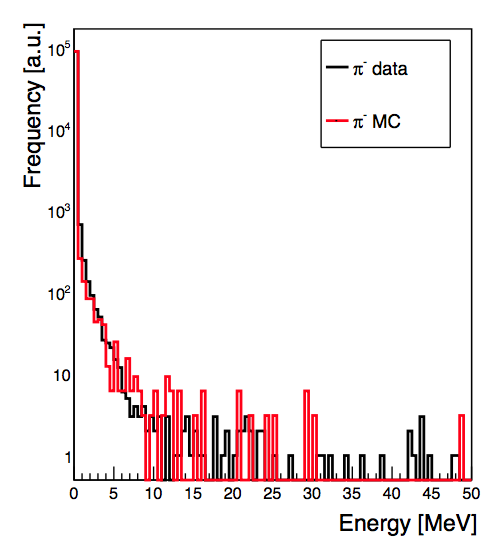
\includegraphics[width=\textwidth]{bgopi.png}
			\caption{}\label{}
		\end{subfigure}
		\hspace*{\fill}
		\caption{}\label{}
\end{figure}
\begin{figure}[ht]
		\centering
		\hspace*{\fill}
		\begin{subfigure}[b]{0.45\textwidth}
			\centering
			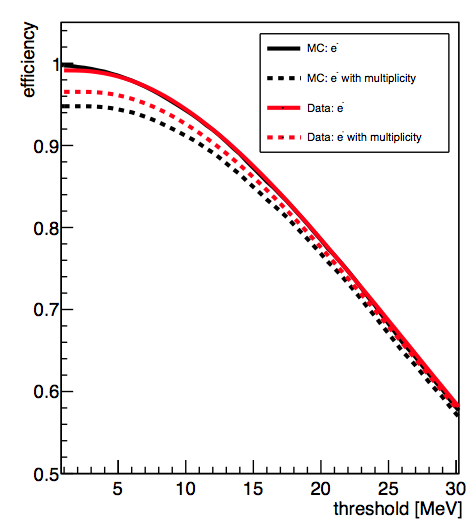
\includegraphics[width=\textwidth]{bgoeff.png}
			\caption{}\label{}
		\end{subfigure}
		\hfill
		\begin{subfigure}[b]{0.45\textwidth}
			\centering
			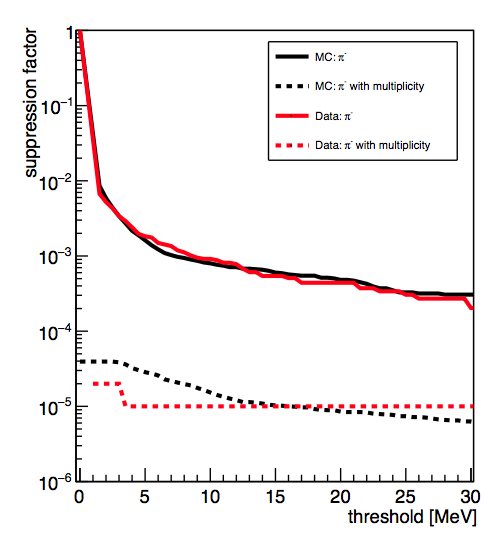
\includegraphics[width=\textwidth]{bgosup.png}
			\caption{}\label{}
		\end{subfigure}
		\hspace*{\fill}
		\caption{}\label{}
\end{figure}

The next two sections show the two equivalent approach for this detector, to calculate the level of hadron suppression
factor. 
\subsection{Total energy}
In the Section \ref{bgoanal}, the level of hadron suppression is calculated using the total energy deposited as
threshold. 


\begin{figure}[ht]
	\hspace*{\fill}
	\centering
	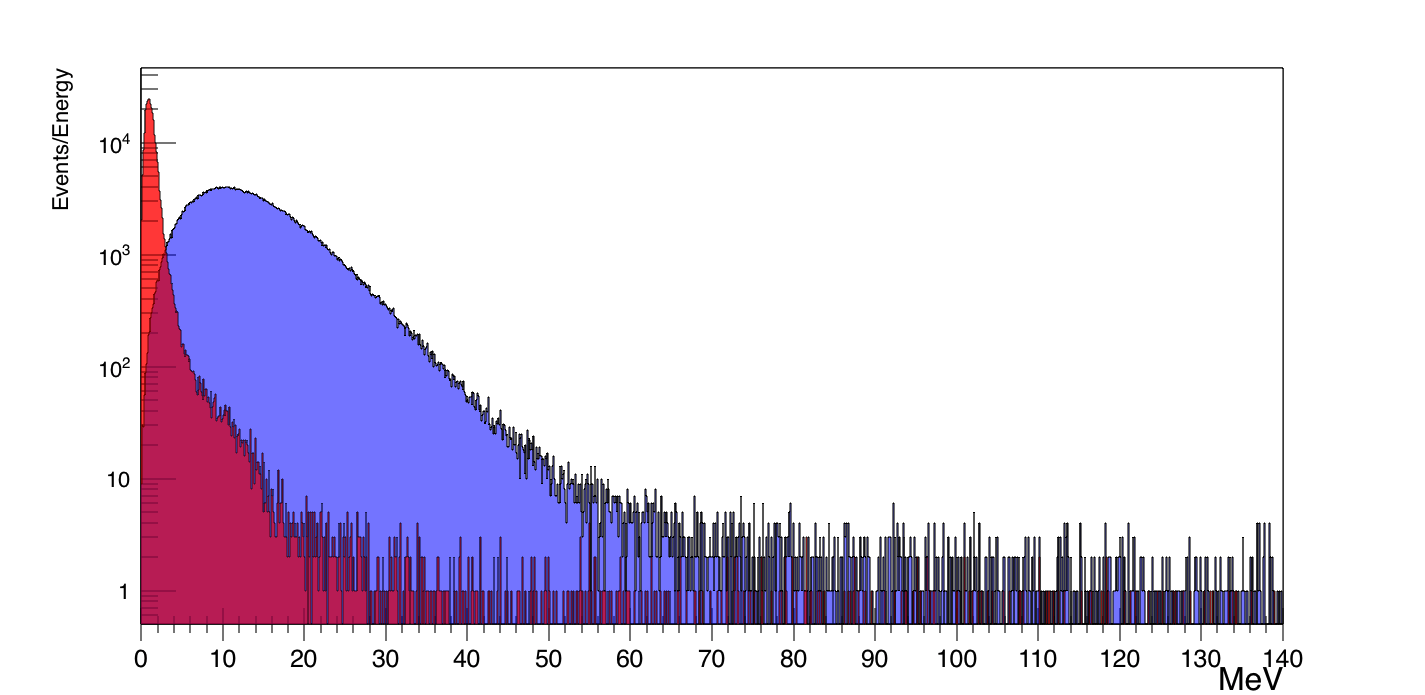
\includegraphics[width=0.9\textwidth]{srdenergy.png}
	\hspace*{\fill}
	\caption{Energy deposition of Synchrotron Radiation configuration. Electrons tagged from $S_{e^-}$ in blue and hadrons
	$S_H$ in red.}\label{srdenergy}
\end{figure}

\begin{figure}[ht]
	\hspace*{\fill}
	\centering
	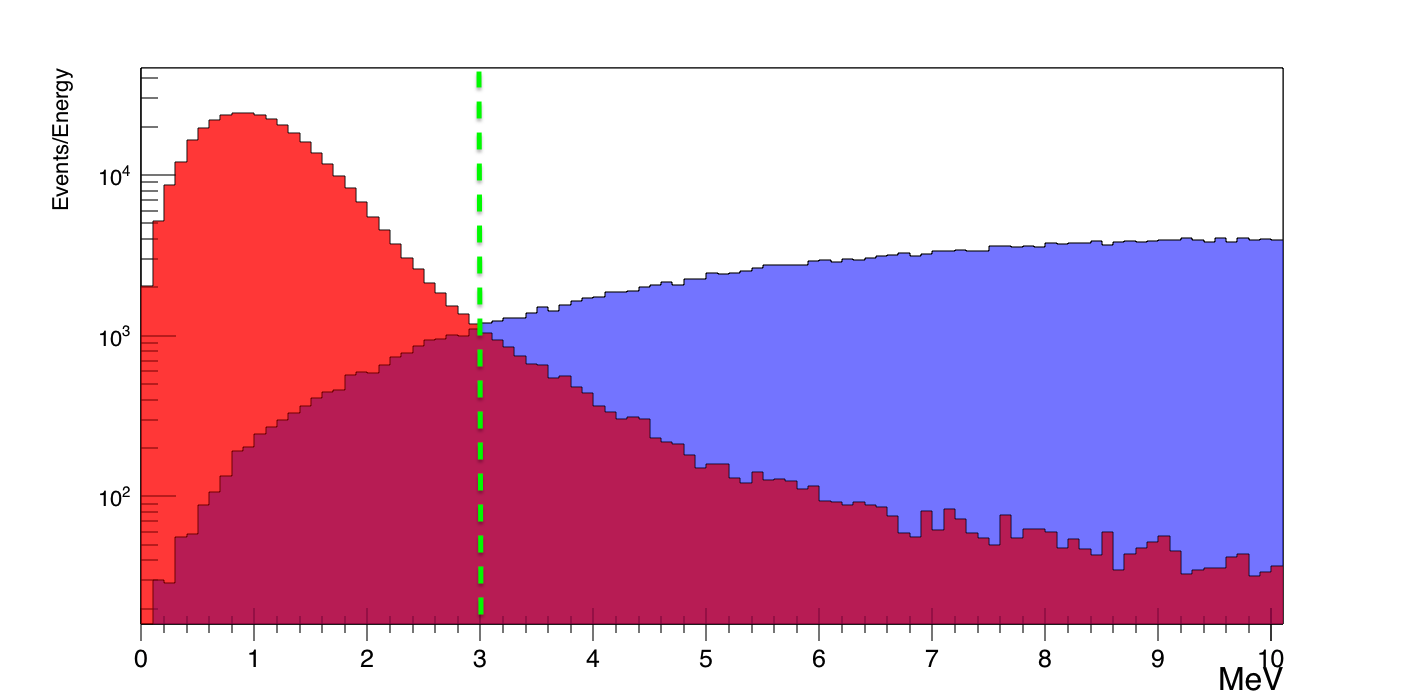
\includegraphics[width=0.7\textwidth]{srdenergyzoom.png}
	\hspace*{\fill}
	\caption{}\label{}
\end{figure}

\begin{figure}[ht]
		\centering
		\hspace*{\fill}
		\begin{subfigure}[b]{0.48\textwidth}
			\centering
			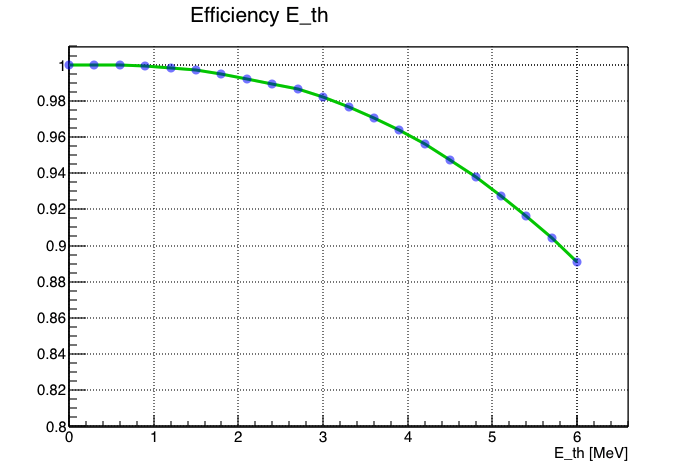
\includegraphics[width=\textwidth]{effE.png}
			\caption{}\label{}
		\end{subfigure}
		\hfill
		\begin{subfigure}[b]{0.48\textwidth}
			\centering
			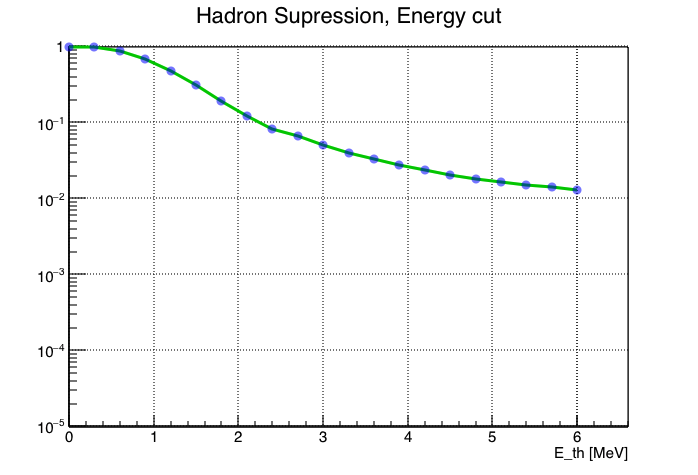
\includegraphics[width=\textwidth]{supE.png}
			\caption{}\label{}
		\end{subfigure}
		\hspace*{\fill}
		\caption{}\label{}
\end{figure}

\begin{figure}[ht]
	\hspace*{\fill}
	\centering
	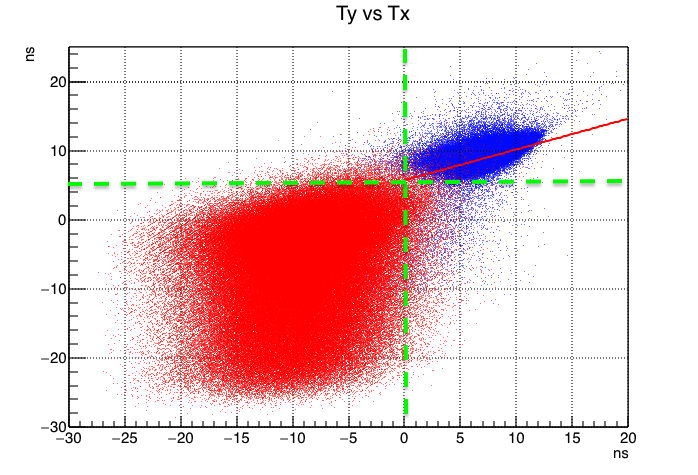
\includegraphics[width=0.8\textwidth]{tytx_fit.png}
	\hspace*{\fill}
	\caption{}\label{}
\end{figure}

\begin{figure}[ht]
		\centering
		\hspace*{\fill}
		\begin{subfigure}[b]{0.48\textwidth}
			\centering
			\includegraphics[width=\textwidth]{effTx.png}
			\caption{}\label{}
		\end{subfigure}
		\hfill
		\begin{subfigure}[b]{0.48\textwidth}
			\centering
			\includegraphics[width=\textwidth]{supTx.png}
			\caption{}\label{}
		\end{subfigure}
		\hspace*{\fill}
		\caption{}\label{}
\end{figure}

\begin{figure}[ht]
		\centering
		\hspace*{\fill}
		\begin{subfigure}[b]{0.48\textwidth}
			\centering
			\includegraphics[width=\textwidth]{effTau.png}
			\caption{}\label{}
		\end{subfigure}
		\hfill
		\begin{subfigure}[b]{0.48\textwidth}
			\centering
			\includegraphics[width=\textwidth]{supTau.png}
			\caption{}\label{}
		\end{subfigure}
		\hspace*{\fill}
		\caption{}\label{}
\end{figure}





\subsection{Strips triggered}




\begin{figure}[ht]
	\hspace*{\fill}
	\centering
	\includegraphics[width=0.7\textwidth]{stripsE.png}
	\hspace*{\fill}
	\caption{}\label{}
\end{figure}


\begin{figure}[ht]
		\centering
		\hspace*{\fill}
		\begin{subfigure}[b]{0.48\textwidth}
			\centering
			\includegraphics[width=\textwidth]{effS.png}
			\caption{}\label{}
		\end{subfigure}
		\hfill
		\begin{subfigure}[b]{0.48\textwidth}
			\centering
			\includegraphics[width=\textwidth]{supS.png}
			\caption{}\label{}
		\end{subfigure}
		\hspace*{\fill}
		\caption{}\label{}
\end{figure}




\section{Experimental Results}

\section{Summary}


